% Desenvolvido por: Prof. Dr. David Buzatto
% Adaptado por: Prof. Dr. Fernando Carvalho
%
% Baseado na documentação do abntex2 e nos modelos em
% Microsoft Word propostos pela Profa. Dra. Rosana F. L. Rodrigues
% e pela bibliotecária M.Sc. Maria Carolina Gonçalves do câmpus
% São João da Boa Vista do IFSP.
%
% Versão 1.5
% Data: 03/09/2018


\documentclass[
	% -- opções da classe memoir --
	12pt,				% tamanho da fonte
	openany,			% capítulos começam em pág ímpar openright (insere página vazia caso preciso)
	oneside,			% para impressão em verso e anverso (twoside). Oposto a oneside 
	a4paper,			% tamanho do papel. 
	normalfigtabnum,
	pnumromarab,
	% -- opções da classe abntex2 --
	chapter=Title,		% títulos de capítulos convertidos em letras maiúsculas
	section=Title,		% títulos de seções convertidos em letras maiúsculas
	%subsection=TITLE,	% títulos de subseções convertidos em letras maiúsculas
	%subsubsection=TITLE,% títulos de subsubseções convertidos em letras maiúsculas
	% -- opções do pacote babel --
	english,			% idioma adicional para hifenização
	french,				% idioma adicional para hifenização
	spanish,			% idioma adicional para hifenização
	brazil,				% o último idioma é o principal do documento
]{abntex2}

% \usepackage{blindtext, showframe}

% \usepackage[a4paper,showframe,
% top    = 2.75cm,
% bottom = 2.50cm,
% left   = 3.00cm,
% right  = 2.50cm]{geometry}


%%%%%%%%%%%%%%%%%%%%%%%%%%%%%%%%%%%%%%%%%%%%%%%%%%%%%%%%%%%%


\newenvironment{conditions}[1][onde:]
  {\noindent
	#1
	
	\indent
	\begin{tabular}[t]{>{$}l<{$} @{${} \> \> {}$} l}}
	{\end{tabular}\\[\belowdisplayskip]}


% --- Controla a geração de listas de siglas, símbolos e glossário
% \RequirePackage[style=long]{glossaries}
% ,long,numberlist


\usepackage[acronyms,symbols]{glossaries}
\setacronymstyle{long-short}

\makenoidxglossaries


%Definição das listas de glossários e parâmertos para compilação.
%-------------------------------------------------------
\newglossary{verbetes}{verbetes}{vrl}{verbetes}
\newglossary{siglas}{siglas}{sgl}{siglas}
\newglossary{simbolos}{simbolos}{sbl}{simbolos}


%Definição dos comandos para exibição das listas individuais.
%-----------------------------------------------------------
\newcommand{\listarsiglas}{\printglossary[type=siglas, title=\listadesiglasname, nonumberlist=true]}
\newcommand{\listarsimbolos}{\printglossary[type=simbolos, title=\listadesimbolosname, nonumberlist=true]}
\newcommand{\listarverbetes}{\printglossary[type=verbetes]}

%Definição dos Comandos para inclusão no texto das siglas.

\newcommand{\verbete}[3]{
	\newglossaryentry{glossary}{name=#1, description={#2}, plural={#3}, type=verbetes}
	\gls{#1}
}

\newcommand{\sigla}[2]{
	\newacronym[type=siglas]{#1}{#1}{#2}
	\gls{#1}
}

\newcommand{\simbolo}[3]{
	\newglossaryentry{#1}{type=simbolos, name=#3, text=#3, description=#2,symbol=#3, sort=def}
	\gls{#1}
}

%%%%%%%%%%%%%%%%%%%%%%%%%%%%%%%%%%%%%%%%%%%%%%%%%%%%%%%%%%%%

\RequirePackage{bookmark}   			



% ---------------------------------------------------------------------------------
%                                   PACOTES
% ---------------------------------------------------------------------------------


% ---
% Pacotes básicos 
% ---

\usepackage{cmap}
\usepackage{lmodern}

\usepackage{amsmath}
\usepackage{latexsym}
\usepackage{amsfonts}
\usepackage[normalem]{ulem}
\usepackage{array}
\usepackage{amssymb}
\usepackage{graphicx}

% \usepackage[backend=bibtex,
% style=authoryear,
% natbib=true,
% sorting=none,
% isbn=false,
% doi=false,
% url=false,

\usepackage{subfig}
\usepackage{wrapfig}
\usepackage{wasysym}
\usepackage{enumitem}
\usepackage{adjustbox}
\usepackage{ragged2e}
\usepackage[svgnames,table]{xcolor}
\usepackage{tikz}
\usetikzlibrary{intersections}
\usetikzlibrary{shapes,arrows,chains}
\tikzstyle{line}=[draw] % here
\usepackage{longtable}
\usepackage{changepage}
\usepackage{setspace}
\usepackage{hhline}
\usepackage{multicol}
\usepackage{tabto}
\usepackage{multirow}
\usepackage{makecell}
\usepackage{fancyhdr}



\usepackage{lmodern}			% Usa a fonte Latin Modern			
\usepackage[T1]{fontenc}		% Selecao de codigos de fonte.
\usepackage[utf8]{inputenc}		% Codificacao do documento (conversão automática dos acentos)
\usepackage{lastpage}			% Usado pela Ficha catalográfica
\usepackage{indentfirst}		% Indenta o primeiro parágrafo de cada seção.
\usepackage{xcolor,colortbl}	% Controle das cores
\usepackage{graphicx}			% Inclusão de gráficos
\usepackage{pgfplots}
\pgfplotsset{compat=1.17}
\usepackage{microtype} 			% para melhorias de justificação
\usepackage{hyperref}
\usepackage{subfig}
\usepackage{epigraph}
\usepackage{url}
\usepackage{placeins}
\usepackage{multirow}
\usepackage[figuresright]{rotating}
\usepackage{chemfig}
\usepackage{amsmath}
\usepackage{amssymb}
\usepackage{enumitem}
\usepackage{bigints}
\usepackage{listings}
\usepackage{etoolbox}
\usepackage[final]{pdfpages}
\usepackage{bigstrut}
\usepackage{makeidx}
\usepackage{float}

% ---



% ---
% Pacotes adicionais, usados apenas no âmbito do Modelo Canônico do abnteX2
% ---
\usepackage{lipsum}				% para geração de dummy text
% ---

% ---
% Pacotes de citações
% ---
\usepackage[brazilian,hyperpageref]{backref}	 % Paginas com as citações na bibl
% \usepackage[alf,abnt-emphasize=bf]{abntex2cite}  % Citações padrão ABNT
\usepackage[alf,abnt-etal-cite=2]{abntex2cite}  % Citações padrão ABNT

% ---------------------------------------------------------------------------------
%                          CONFIGURAÇÕES DOS PACOTES
% ---------------------------------------------------------------------------------

% ---
% Configurações do pacote backref
%
% Para desativar, tire o comentário de \begin{comment} e \end{comment} 
% das próximas linhas e comente a linha \usepackage[brazilian,hyperpageref]{backref}
% acima.
% ---

% \newcommand{\imprimirdata}{\data}


%\begin{comment}
% ---
% Configurações do pacote backref
% Usado sem a opção hyperpageref de backref
\renewcommand{\backrefpagesname}{Citado na(s) página(s):~}
% Texto padrão antes do número das páginas
\renewcommand{\backref}{}
% Define os textos da citação
\renewcommand*{\backrefalt}[4]{
	\ifcase #1 %
	Nenhuma citação no texto.%
	\or
	Citado na página #2.%
	\else
	Citado #1 vezes nas páginas #2.%
	\fi}%
% ---
%\end{comment}


% listagens
\definecolor{corComentario}{RGB}{150,150,150}
\definecolor{corString}{RGB}{206,123,0}
\definecolor{corPalavraChave}{RGB}{0,0,230}

\lstset{
	numbers=left,
	stepnumber=1,
	firstnumber=1,
	numberstyle=\footnotesize,
	extendedchars=true,
	breaklines=true,
	lineskip=0pt,
	frame=tb,
	basicstyle=\ttfamily\footnotesize,
	showstringspaces=false,
	stringstyle=\color{corString},
	commentstyle=\color{corComentario},
	keywordstyle=\color{corPalavraChave}
}

\newcommand{\graficoname}{Gráfico}
\newcommand{\graficorefname}{Gráfico}
\newcommand{\listofgraficosname}{Lista de gráficos}





% \newcolumntype{Y}{>{\centering\arraybackslash}X}

\newcommand{\ano}[1]{\def \oano {#1}}
\newcommand{\imprimirano}{\oano}

\newcommand{\mes}[1]{\def \omes {#1}}
\newcommand{\imprimirmes}{\omes}

\newcommand{\dia}[1]{\def \odia {#1}}
\newcommand{\imprimirdia}{\odia}

% \newcommand{\subtitulo}[1]{\def \osubtitulo {#1}}
% \newcommand{\imprimirsubtitulo}{\osubtitulo}

\newcommand{\area}[1]{\def \aarea {#1}}
\newcommand{\imprimirarea}{\aarea}

\newcommand{\disciplina}[1]{\def \adisciplina {#1}}
\newcommand{\imprimirdisciplina}{\adisciplina}

% \renewcommand{\coorientador}[1]{\def \ocoorientador {#1}}
% \renewcommand{\imprimircoorientador}{\ocoorientador}

\newcommand{\grau}[1]{\def \ograu {#1}}
\newcommand{\imprimirgrau}{\ograu}

\newcommand{\curso}[1]{\def \ocurso {#1}}
\newcommand{\imprimircurso}{\ocurso}

\newcommand{\campus}[1]{\def \ocampus {#1}}
\newcommand{\imprimircampus}{\ocampus}


% Área de Concentração: \imprimirarea}
% ---


% ---
% Configurações de aparência do PDF final
% ---

% alterando o aspecto da cor azul
\definecolor{blue}{RGB}{41,5,195}

% informações do PDF
\makeatletter
\hypersetup{
	%pagebackref=true,
	pdftitle={\@title}, 
	pdfauthor={\@author},
	pdfsubject={\imprimirpreambulo},
	pdfcreator={\@author},
	pdfkeywords={Palavra chave 1}{Palavra chave 2}{Palavra chave 3}{Palavra chave n}, 
	colorlinks=true,       		% false: boxed links; true: colored links
	linkcolor=blue,          	% color of internal links
	citecolor=blue,       		% color of links to bibliography
	filecolor=black,      		% color of file links
	urlcolor=blue,
	bookmarksdepth=4
}
\makeatother
% --- 


% ---
% Comandos do autor
% ---

% comando para inserir autor e ano
\newcommand{\citeauthorandyear}[1]{\citeauthoronline{#1} (\citeyear{#1})}

% --- 
% Espaçamentos entre linhas e parágrafos 
% --- 

% O tamanho do parágrafo é dado por:
\setlength{\parindent}{1.3cm}

% Controle do espaçamento entre um parágrafo e outro:
\setlength{\parskip}{0.2cm}  % tente também \onelineskip

\glsaddall

% ---
% compila os glossários e listas
% \makeglossaries

% ---
% compila o indice
% ---
\makeindex
% ---
%---


%%%%%%%%%%%%%%%%%%%%%%%%%%%%%%%%%%%%%%%%%%%%

% para o pacote "Lst Listing"

\newcommand{\source}[1]{\caption*{Fonte: {#1}}}

% Altera o nome padrão do rótulo usado no comando \autoref{}
\renewcommand{\lstlistingname}{Código}

% Altera o rótulo a ser usando no elemento pré-textual "Lista de código"
\renewcommand{\lstlistlistingname}{Lista de códigos}

%% Configuração para o ambiente de código (algorítmos)
\lstset{
%   numbers=left,
%   inputencoding=latin1,
%   basicstyle=\footnotesize\ttfamily,
%   keywordstyle=\color{blue},         
%   breaklines=true, 
%   showtabs=false,
%   showstringspaces=false,
%   numberstyle=\tiny\color{mygray}
   basicstyle=\fontsize{9}{11}\selectfont\ttfamily
}
%% 
%% exemplo da página https://latex.org/forum/viewtopic.php?t=24038
%%

% comandos para excluir items da table of contents (Sumário)
\let\oldaddcontentsline\addcontentsline
\newcommand{\hidefromtoc}{\renewcommand{\addcontentsline}[3]{}}
\newcommand{\writetotoc}{\let\addcontentsline\oldaddcontentsline}
\newacronym{dvd}{DVD}{Digital Versatile Disc}
\newacronym{ddd}{DDD}{Domain-Driven Design}
\newacronym{soa}{SOA}{Service-Oriented Architecture}
\newacronym{poo}{POO}{Programação Orientada a Objetos}
\newacronym{cpu}{CPU}{Central Processing Unit}
\newacronym{ide}{IDE}{Integrated Development Environment}
\newacronym{ipc}{IPC}{Inter-Process Communication}
\newacronym{lgpd}{LGPD}{Lei Geral de Proteção de Dados Pessoais}
\newacronym{ohs}{OHS}{Open Host Service}
\newacronym{acl}{ACL}{Anti-Corruption Layer}
\newacronym{api}{API}{Application Programming Interface}
\newacronym{bc}{BC}{Bounded Context}
\newacronym{ams}{AMS}{Arquitetura de Microsserviços}
\newacronym{vo}{VO}{Value Object}
\newacronym{acid}{ACID}{Atomicidade, Consistência, Isolamento e Durabilidade}



% ---------------------------------------------------------------------
% Informações de dados para CAPA, FOLHA DE ROSTO e FOLHA DE ASSINATURAS
% ---------------------------------------------------------------------

% ---------------------------------------------------------------------
% Alterar os dados abaixo com os seus dados
%
% obs: Os nomes e instituições dos membros da banca deverão ser
%       alterados no arquivo 03-assinaturas.tex 
% ---------------------------------------------------------------------

\curso{Bacharelado em Sistemas de Informação}
\grau{Bacharel em Sistemas de Informação} 
\titulo{Proposta de \english{Design} para uma locadora de carros: uma abordagem baseada em \english{Domain-Driven Design} e Microsserviços}
\tipotrabalho{Trabalho de Conclusão}
\area{Tecnologia da Informação}

\autor{Raphael Collin Teles Manhães}
\orientador{Prof. D.Sc. Mark Douglas de Azevedo Jacyntho}

% caso não haja coorientador, comente a linha abaixo
% \coorientador{Profa. M.Sc. Nome da Professora Coorientadora}

\local{Campos dos Goytacazes-RJ}
\dia{29}
\mes{abril}
\ano{2024}
\data{Abril de \imprimirano}

\instituicao{Instituto Federal de Educação, Ciência e Tecnologia Fluminense}
\campus{Campos-Centro}

\preambulo{\imprimirtipotrabalho\ apresentado ao curso \imprimircurso~ do \imprimirinstituicao, como parte dos requisitos para a obtenção do título de \imprimirgrau.}

% ---------------------------------------------------------------------------------
%                                   INÍCIO DO DOCUMENTO
% ---------------------------------------------------------------------------------

\begin{document}

\pretextual

\begin{capa}
\imprimircapa 
\end{capa}


\imprimirfolhaderosto{}


% ---
% Inserir folha de aprovação
% ---

% Isto é um exemplo de Folha de aprovação, elemento obrigatório da NBR
% 14724/2011 (seção 4.2.1.3). Você pode utilizar este modelo até a aprovação
% do trabalho. Após isso, substitua todo o conteúdo deste arquivo por uma
% imagem da página assinada pela banca com o comando abaixo:
%
%\begin{folhadeaprovacao}
%	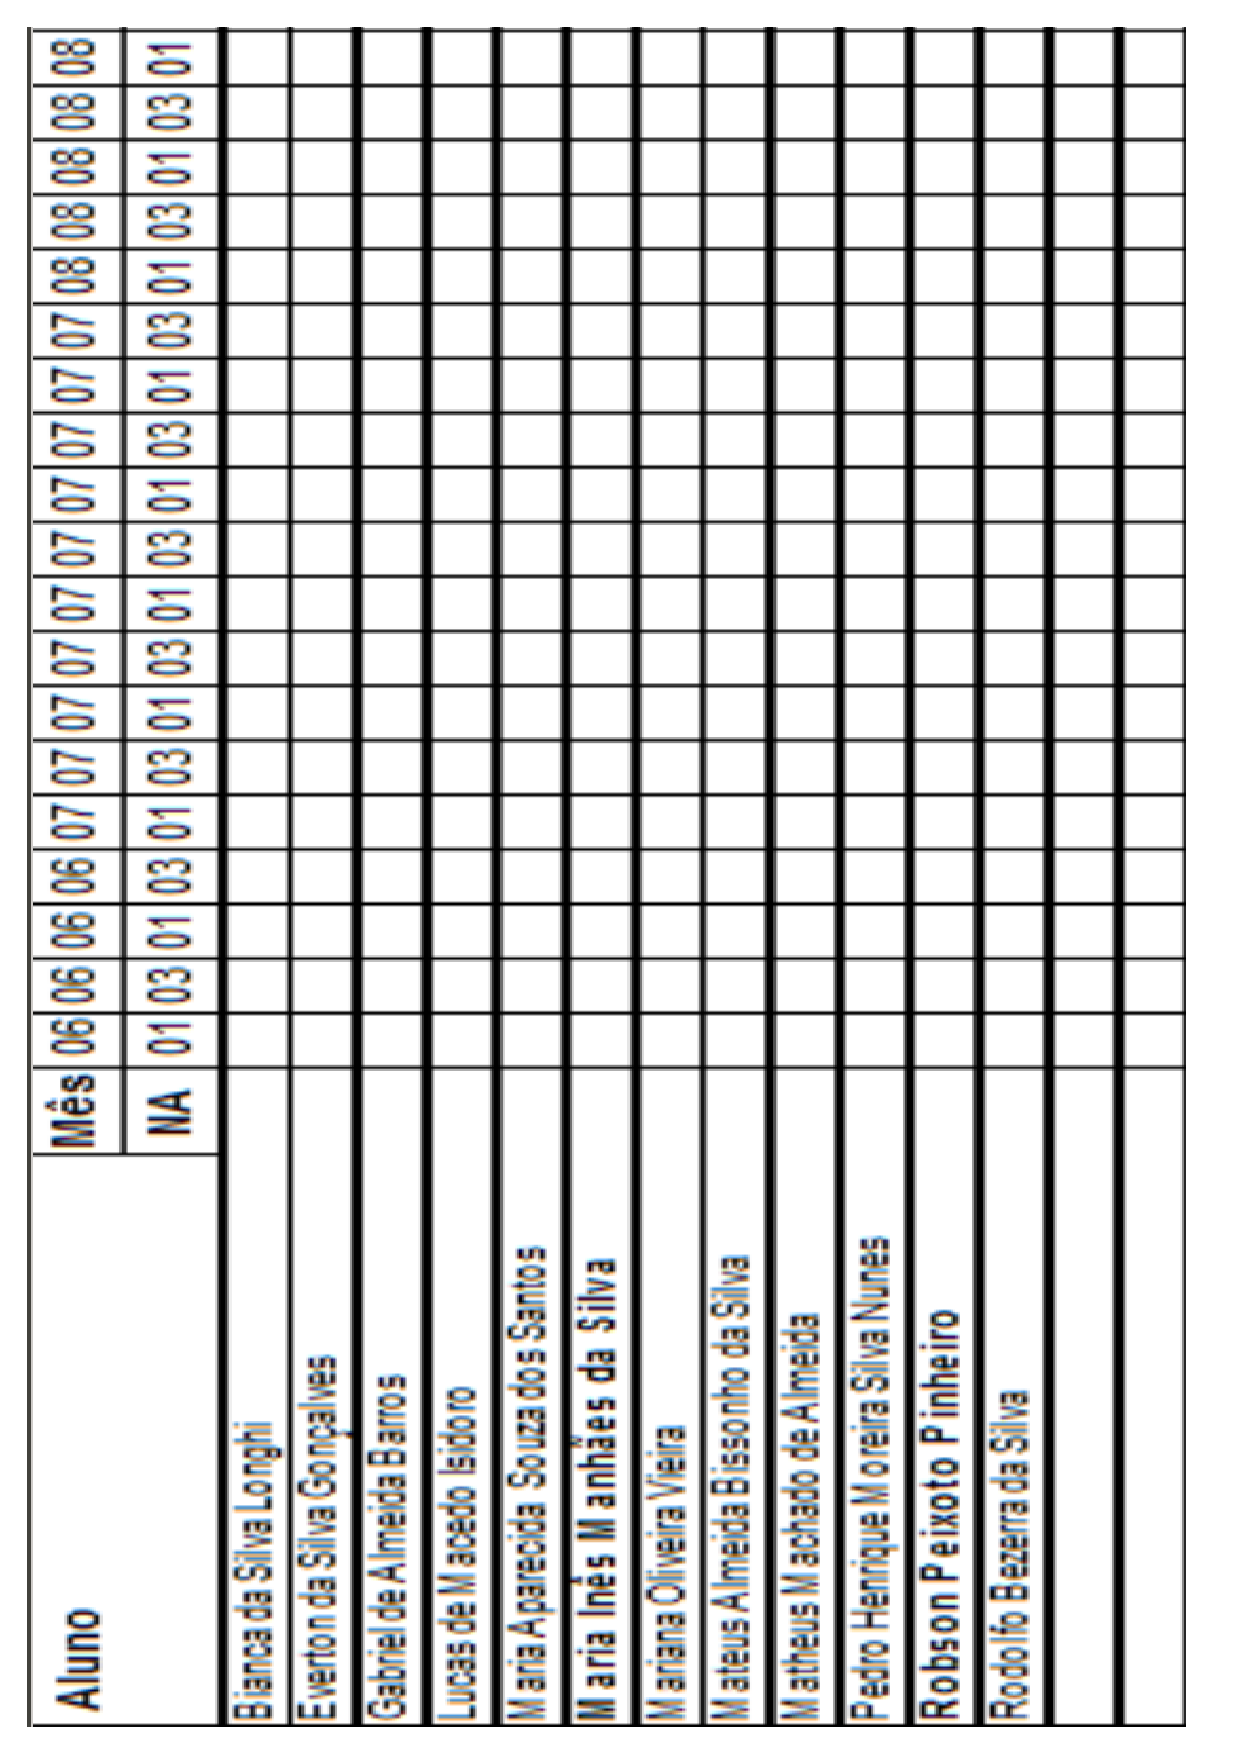
\includepdf{pre/FolhaAprovacaoAssinada}
%\end{folhadeaprovacao}

%
\begin{folhadeaprovacao}

\setlength{\ABNTEXsignwidth}{14cm}

    \begin{center}
    {\ABNTEXchapterfont\large\imprimirautor}

    \vspace*{\fill}\vspace*{\fill}
    {\ABNTEXchapterfont\bfseries\Large\imprimirtitulo}
    \vspace*{\fill}
    
    \hspace{.45\textwidth}
    \begin{minipage}{.5\textwidth}
        \imprimirpreambulo
    \end{minipage}%
    \vspace*{\fill}
   
   \end{center}
 
 
   \begin{center}
    \imprimirlocal, \imprimirdia ~de \imprimirmes ~de \imprimirano.
   \end{center}
   
   % Instituto Federal Fluminense (IFF)
   \assinatura{\textbf{Prof. M.Sc. Nome do Primeiro Professor} \\ Instituto Federal Fluminense (IFF)}
   \assinatura{\textbf{Prof. D.Sc. Nome do Segundo Professor} \\ Universidade Estadual do Norte Fluminense - Darcy Ribeiro (UENF)}
   \assinatura{\textbf{\imprimirorientador} \\ Instituto Federal Fluminense (IFF)}
   \assinatura{\textbf{\imprimircoorientador} \\ Instituto Federal Fluminense (IFF)}

   \begin{center}
    \vspace*{0.5cm}
    {\ABNTEXchapterfont\large\imprimirlocal}
    \par
    {\ABNTEXchapterfont\large\imprimirdata}
    \vspace*{1cm}
  \end{center}
  
\end{folhadeaprovacao}
% ---



\begin{agradecimentos}

Em primeiro lugar, agradeço a Deus por ter me dado força e sabedoria para superar os desafios e dificuldades ao longo da minha jornada acadêmica.

Agradeço também a minha mãe que sempre me apoiou e incentivou a seguir em frente na vida acadêmica e profissional desde os primeiros momentos. Sou muito grato por todo o amor, carinho e dedicação que sempre me proporcionou. Se hoje estou aqui, é graças a você.

Agradeço ao meu orientador, Prof. Dr. Mark Douglas, por todo o apoio, orientação e ensinamentos durante suas aulas, nossas conversas e ao longo deste trabalho. Sua paciência, dedicação e conhecimento foram fundamentais para o desenvolvimento deste estudo.

Por fim, sou extramente grato a todos professores, autores, colegas e amigos que em algum momento me ensinaram algo e contribuíram para a minha formação acadêmica e profissional. Acredito firmemente que a educação é a chave para não apenas para atingir nossos objetivos pessoais, mas também para transformar nosso país e o mundo em um lugar mais próspero, solidário e justo. 

\end{agradecimentos}




\begin{resumo}

% O comando lipsum abaixo é um gerador automático de texto.
% Substitua-o pelo texto do seu resumo.
% Lembre-se: Um resumo deve ser um parágrafo único que apresente os seguintes tópicos:

% Contexto;
% Problema;
% Objetivo;
% Justificativa;
% Metodologia;
% Resultado;
% Conclusão.

Com a popularização da computação em nuvem, a crescente demanda de mudanças cada vez mais frequentes e o crescimento das equipes de tecnologia da informação em grandes organizações, a arquitetura tradicional para o desenvolvimento de aplicações corporativas, baseada em monólitos, é confrontada com desafios significativos. Nesse cenário, surge como alternativa a Arquitetura de Microsserviços. Paralelamente a isso, a abordagem \textit{Domain-Driven Design} (DDD) tem sido cada vez mais utilizada para modelagem de domínios de negócio complexos. Essas duas estratégias podem ser combinadas no \textit{design} e desenvolvimento de sistemas. De um lado, microsserviços possibilitam escalabilidade independente, implantação desacoplada e utilização de múltiplas tecnologias para determinados casos de uso. Por outro lado, DDD fornece uma abordagem para modelagem do domínio de negócio, diversos padrões para resolver problemas de modelagem recorrentes e facilidade de entendimento e manutenção de código. Além disso, DDD é uma excelente estratégia para definição de limites entre microsserviços. No entanto, a utilização combinada desses dois conceitos apresenta nuances e diferentes possibilidades. Assim, esse trabalho apresenta um estudo de caso realista de uma locadora de veículos com o emprego dessas estratégias visando oferecer uma contribuição significativa para a compreensão da aplicação integrada dessas abordagens.

\textbf{Palavras-chaves: } Microsserviços, \textit{Domain-Driven Design}, Arquitetura de Microsserviços.  

\end{resumo}




\begin{resumo}[Abstract]
 \begin{otherlanguage*}{english}

% O comando lipsum abaixo é um gerador automático de texto, e deve ser substituído pelo seu abstract.

Considering the popularization of cloud computing, the increasing demand for more frequent changes and the growth of information technology teams in large organizations, the traditional architecture for developing enterprise applications, based on monoliths, is confronted with significant challenges. In this scenario, the Microservices Architecture emerges as an alternative. At the same time, the Domain-Driven Design (DDD) methodology has been increasingly used to model complex business domains. These two strategies can be combined in the design and development of systems. On one side, microservices enable independent scalability, decoupled deployment, and the use of multiple technologies for certain use cases. On the other hand, DDD provides an approach to modeling the business domain, several patterns to solve recurring modeling problems, and ease of understanding and maintaining code. In addition, DDD is an excellent strategy for defining boundaries between microservices. However, the combined use of these two concepts faces nuances and different possibilities. Therefore, this work presents a realistic case study of a vehicle retailer  with the use of these strategies aiming to offer a significant contribution to the understanding of the integrated application of these approaches.

\textbf{Keywords: } Microservices, Domain-Driven Design, Microservices Architecture.

\end{otherlanguage*}
\end{resumo}



% não é necessário alterar este arquivo

\listoffigures*
\clearpage


% não é necessário alterar este arquivo

\listofquadros
\clearpage


% não é necessário alterar este arquivo

\listoftables*
\clearpage


% não é necessário alterar este arquivo

\listofcodigos*
\clearpage




% \printglossaries
\printglossary

\setglossarypreamble[acronym]{%
	\glsresetentrycounter
}
\setglossarystyle{long3col}
\printnoidxglossary[type=acronym]

\clearpage



\setglossarypreamble[symbols]{%
	\glsresetentrycounter
}

\setglossarystyle{long3col}

\printnoidxglossary[type=symbols]

\clearpage



 %%%%%%%%%%%%  This Produces Table Of Contents %%%%%%%%%%%%%%

\vspace{\baselineskip}
\setlength{\parskip}{0.0pt}

\begin{Center}
\end{Center}\par


\vspace{\baselineskip}
\setlength{\parskip}{9.96pt}


\tableofcontents*

\clearpage

 %%%%%%%%%%%%  Starting New Page here %%%%%%%%%%%%%%


\textual

\chapter{Introdução}
\label{cap:introducao}

\section{Problema e contexto}

A abordagem convencional no desenvolvimento de sistemas corporativos, na qual toda a lógica de negócio, persistência e apresentação são encapsuladas em uma única aplicação (e um único executável), é a mais natural para construção desse tipo de sistema. Essa arquitetura, conhecida comumente como monólito, tem alcançado sucesso devido à sua simplicidade no desenvolvimento, testes, implantação e monitoramento, entre outros fatores. No entanto, com a popularização da computação em nuvem, a crescente demanda de mudanças cada vez mais frequentes e o crescimento das equipes de tecnologia da informação em grandes organizações, essa arquitetura é confrontada com desafios significativos. Inicialmente, destaca-se o acoplamento nos ciclos de mudanças, onde qualquer alteração em uma pequena parte requer a compilação e implantação de todo sistema. Além disso, há dificuldade em escalar horizontalmente apenas funcionalidades específicas que estão sendo mais demandas e existe complexidade na utilização de diferentes linguagens de programação em diversas áreas de um sistema \cite{microservices}. Por esses motivos, a adoção da \acrlong{ams} cresceu de forma exponencial nos últimos anos, com 77\% dos profissionais afirmando que suas organizações utilizam esse estilo arquitetural \cite{microserviceAdoption}.

Por outro lado, \english{\acrfull{ddd}} é uma abordagem para o desenvolvimento de software, na qual os elementos de software como pacotes, classes, interfaces, métodos e nomes de variáveis devem corresponder aos conceitos do domínio de negócio \cite{dddFowler}. Adicionalmente, o \acrshort{ddd} se configura como uma estratégia para harmonizar especialistas de negócios, desenvolvedores e projetistas, promovendo uma otimização nas interações ao reduzir o mapeamento entre termos de negócio e termos técnicos.

Em agosto de 2008, um grande incidente interrompeu as operações da \emph{Netflix}, empresa que nesse período alugava \acrshort{dvd}s através de seu site na \english{web}. Uma corrupção no banco de dados impediu que a companhia pudesse realizar envios por três dias. A partir desse momento, os engenheiros perceberam que necessitavam reduzir pontos únicos de falha, tais como grandes bases de dados relacionais armazenadas em somente um \english{data center}. Em vez disso, optaram por adotar sistemas distribuídos na nuvem, escalonados horizontalmente, para garantir maior confiabilidade e minimizar o impacto das falhas \cite{netflixMigration}.

Essa transição resultou em vários benefícios para a \emph{Netflix}, destacando-se a conquista de uma disponibilidade de 'quatro noves' (99,99\%) e significativa redução de custos. Além disso, a \acrfull{ams} permitiu que diferentes aplicações utilizassem diferentes tecnologias, facilitando contratações e extraindo o melhor de cada opção. Assim, em 2016 (8 anos após a migração) a empresa tinha 8 vezes mais assinantes, muito mais ativos, com o número de visualizações crescendo em três ordens de grandeza nesse período \cite{netflixMigration}.

A \acrfull{ams} e \acrshort{ddd} podem ser combinados no \english{design} e desenvolvimento um sistema. De um lado, microsserviços possibilitam escalabilidade independente, implantação desacoplada e utilização de múltiplas tecnologias para determinados casos de uso. Por outro lado, \acrshort{ddd} fornece uma abordagem para modelagem do domínio de negócio, diversos padrões para resolver problemas de modelagem recorrentes e facilidade de entendimento e manutenção de código. Além disso, \acrshort{ddd} é uma excelente estratégia para definição de limites entre microsserviços. Ao modelar os serviços com base em \english{\acrlong{bc}}s coesos, é possível o desenvolvimento de novas funcionalidades mais rapidamente e também se torna mais simples a recombinação de microsserviços para fornecer novas funcionalidades aos usuários \cite{buildingMicroservices}.

\section{Justificativa}

Recentemente, observou-se um notável crescimento em popularidade e adoção da \acrshort{ams} e da abordagem \english{\acrfull{ddd}} no desenvolvimento de sistemas corporativos. Porém, essas tecnologias são utilizadas de maneira equivocada em muitas implementações devido à falta de compreensão das suas vantagens e desvantagens, entre outros fatores. Por exemplo, a equipe de desenvolvimento do \emph{Amazon Prime Video} recentemente anunciou uma migração de um serviço de monitoramento de vídeo, que foi inicialmente desenvolvido com microsserviços, para uma arquitetura monolítica com objetivo de aumentar a escalabilidade e reduzir custos \cite{amazonBackMigration}.

Paralelamente a isso, é possível identificar uma carência de estudos de caso realistas envolvendo a utilização simultânea da \acrshort{ams} e \english{\acrfull{ddd}}, especialmente no cenário nacional.  Enquanto algumas publicações concentram-se exclusivamente em um desses conceitos e outras apresentam exemplos simplificados, proporcionando uma compreensão limitada de como essas duas técnicas podem ser efetivamente empregadas em conjunto. 

Nesse contexto, este trabalho visa preencher essa lacuna ao oferecer uma contribuição significativa para a compreensão da aplicação integrada dessas estratégias no desenvolvimento de sistemas. Por meio de um estudo de caso realista, busca-se não apenas enriquecer o conhecimento acadêmico, mas também fornecer uma base sólida para a implementação prática dessas tecnologias em diversos setores da indústria.

\section{Objetivos}

\subsection{Objetivo Geral}
O objetivo geral deste trabalho de conclusão de curso é apresentar uma proposta de integração da \acrlong{ams} e \acrlong{ddd} no desenvolvimento de aplicações visando ganhos de flexibilidade, escalabilidade e em manutenibilidade com um estudo de caso realista para um sistema de locação de veículos.

\subsection{Objetivos Específicos}
\begin{itemize}
\item Apresentar estratégia para transformar requisitos funcionais em um \english{design} funcional com \acrshort{ams} e \acrshort{ddd}.
\item Prover informações relevantes para tomada de decisões técnicas com essas tecnologias.
\item Realizar uma implementação funcional do \english{design}.
\end{itemize}

\section{Estrutura do Trabalho}

Este trabalho está dividido em sete capítulos.  O \autoref{cap:introducao} expõe o contexto do estudo, as justificativas desta pesquisa e os objetivos a serem atingidos. O \autoref{cap:fundamentacao} apresenta conceitos de caracterização de materiais, relata algumas normas de organizações internacionais para este fim e faz uma explanação sobre a área de processamento e análise de imagens. O \autoref{cap:trabalhos}... . Finalmente, o \autoref{cap:conclusão} apresenta a conclusão e os potenciais trabalhos futuros a serem desenvolvidos.

\chapter{Fundamentação Teórica}
\label{cap:fundamentacao}

Este capítulo apresenta os conceitos de Sistemas Distribuídos, \acrfull{soa} Microsserviços, \acrshort{ddd} e Arquitetura Hexagonal.

\section{\english{Domain-Driven Design (DDD)}} 
\english{\acrfull{ddd}} é uma abordagem para o desenvolvimento de software focada na construção de um modelo de domínio que representa de maneira sofisticada os processos e regras de negócio do sistema em questão \cite{dddFowler}. \acrshort{ddd} é muito efetivo para desenvolver sistemas com regras de negócio complexas, que possuem, por exemplo, diversos atores, entidades e validações. A \acrfull{poo} é geralmente empregada para a implementação do modelo de domínio, visto que possui uma série de recursos que facilitam a modelagem de objetos do mundo real \cite{evans2004ddd}.

Um ponto central da metodologia \acrshort{ddd}, no desenvolvimento de softwares complexos, é a utilização de uma linguagem ubíqua que insere terminologia e jargões do domínio em componentes de software como atributos, métodos, classes, interfaces e pacotes \cite{dddFowler}. Assim, tanto especialistas de negócio quanto desenvolvedores e projetistas compartilham um vocabulário comum que facilita na comunicação e reduz a necessidade de realizar o mapeamento entre termos técnicos e termos do domínio. Além disso, a estrutura de sistema passa a representar a estrutura do negócio, tornando-se, assim, mais fácil de ser compreendida e modificada.

O nome dessa estrategia vem de um livro publicado em \citeyear{evans2004ddd} por Eric Evans que descreve a abordagem, uma série de conceitos e um catálogo de  padrões comumente utilizados para resolução de problemas de modelagem de domínios. Os mais relevantes dentre estes são descritos a seguir.

\subsection{Modelo e Domínio}
Os conceitos de modelo e domínio, no contexto da engenharia de software, são fundamentais para o entendimento do \acrshort{ddd}. Modelo é uma simplificação, uma interpretação da realidade que abstrai os aspectos relevantes para resolver o problema em questão e ignora detalhes superficiais \cite{evans2004ddd}. Da mesma forma, todo sistema computacional está relacionado a alguma atividade ou interesse do usuário final. Assim, a área para qual o usuário utiliza o sistema é domínio do software \cite{evans2004ddd}. Alguns exemplos de domínios comuns são: financeiro, médico, logística e \english{marketplace}.

\subsection{Entidade}
No contexto da \acrshort{poo}, muitos objetos não são fundamentalmente definidos por seus atributos, mas por um fio de continuidade e identidade \cite{evans2004ddd}. Eles podem ter distintas representações como, por exemplo, em memória ou em um banco de dados. No entanto, eles necessitam ser distinguíveis mesmo se todas suas propriedades forem iguais. Em um domínio financeiro, por exemplo, uma transação composta por valor, data e usuário necessita ser diferenciável de outra transação com as mesmas características. Por outro lado, para uma classe fictícia chamada \english{Money} composta por valor e moeda, dois objetos com os mesmos atributos podem ser geralmente considerados iguais, sem gerar corrupções de dados ou impactos para os usuários finais do sistema. Em resumo, quando um objeto definido principalmente por sua identidade, ele é chamado de Entidade \cite{evans2004ddd}.

\subsection{\english{\acrfull{vo}}}
Muitos objetos não possuem identidade conceitual, sendo somente utilizados para descrever características de outro objeto. São objetos que descrevem coisas, classificados como \acrshort{vo} \cite{evans2004ddd}. Para um sistema de uma loja de roupas, por exemplo, um objeto que representa cor de cada peça formado pelas propriedades \english{red}, \english{green} e \english{blue}, não possui identidade. Não necessita ser diferenciável de outro objeto com as mesmas propriedades. Este objeto somente descreve uma característica de uma peça de roupa. É importante ressaltar, porém, que a diferenciação entre Entidade e \english{\acrlong{vo}} depende do contexto do software. Para um sistema de software de computação gráfica, a cor é um conceito chave no sistema e pode possuir identidade.

Pode-se pensar que é mais vantajoso sempre projetar os objetos do sistema como Entidade, pois adicionaria identidade, facilitaria o rastreamento de mudanças e agregaria mais recursos ao objeto. No entanto, a adição de identidade para objetos que não necessitam desta classificação pode prejudicar o desempenho do sistema, adicionar mais esforço de análise e aumentar a complexidade do modelo de domínio \cite{evans2004ddd}. Por esse motivo, recomenda-se a utilização de \acrshort{vo} sempre que for possível, pois se tratam de objetos mais fáceis de gerenciar.

\subsection{Serviço}
Em muitos casos, há operações importantes no modelo que não pertencem conceitualmente a nenhuma Entidade ou \acrshort{vo}. Dessa forma, surge o conceito de Serviço: uma operação fornecida como uma interface autônoma no modelo, sem encapsular estado como outros tipos de objeto \cite{evans2004ddd}.

Um erro comum é a abusar da utilização de Serviços, desistindo de encontrar o objeto apropriado para uma operação de domínio. Da mesma forma, a inserção de um método que não está alinhado com a definição do objeto resulta na perda de coesão desse objeto, tornando-o mais difícil de compreender e refatorar \cite{evans2004ddd}. Considerando esses pontos, um serviço deve ser utilizado quando um processo ou transformação relevante no modelo de domínio não faz parte da responsabilidade natural de uma Entidade ou \acrshort{vo}.

Além disso, \citeonline{evans2004ddd} destaca três características de um bom Serviço:
\begin{itemize}
    \item A operação não possui estado (\english{stateless}).
    \item A interface é defina em termos de outros elementos do modelo de domínio.
    \item A operação se relaciona a um conceito do modelo que não é parte natural de uma Entidade ou \acrshort{vo}.
\end{itemize}

\subsection{\textit{Aggregate}}
\label{section:aggregate}
Um \english{Aggregate} é um conjunto de objetos associados, tratados como uma única unidade para o proposito de alterações de dados \cite{evans2004ddd}. Em um sistema de grande porte, é difícil garantir a consistência de alterações em objetos com relacionamentos complexos. As invariantes que precisam ser mantidas geralmente envolvem um grupo de objetos intimamente associados, ao invés de objetos isolados. Assim, o padrão \english{Aggregate} propõe delimitações definidas e restrições de acesso visando o melhor tratamento das associações entre objetos.

Cada \english{Aggregate} possui uma raiz e uma delimitação, que define o que está dentro do \english{Aggregate} \cite{evans2004ddd}. A raiz é a única entidade global - que possui identidade em todo o sistema - contida dentro do \english{Aggregate}, também conhecida como \english{Aggregate root} \cite{evans2004ddd}. Objetos fora da delimitação do \english{Aggregate} só podem possuir referências a raiz e não a outros objetos dentro do \english{Aggregate}. Excluindo a raiz, outras entidades somente possuem identidade local, necessitando somente ser distinguíveis dentro dos limites do \english{Aggregate}, visto que nenhum objeto de fora consegue obtê-las desassociadas da entidade raiz \cite{evans2004ddd}.

\subsection{\acrfull{bc}}
\label{section:bounded_context}
Em grandes projetos, muitos modelos coexistem em diferentes contextos. Quando a base de código, no entanto, combina diferentes modelos sem que haja uma separação clara, o \english{software} se torna defeituoso, frágil e difícil de ser compreendido \cite{evans2004ddd}. Assim, é necessário especificar em qual o contexto um determinado modelo está sendo aplicado.  Assim, um \acrshort{bc} delimita a aplicabilidade de um modelo, de tal forma que os membros da equipe tenham um entendimento claro do que precisa ser consistente e a relação do modelo com outros contextos. Um \acrshort{bc} engloba tanto componentes de modelo como \english{Aggregates}, Entidades, \english{\acrlong{vo}}s e Serviços, quanto detalhes técnicos como persistência. É uma parte completa e funcional de software sob responsabilidade de uma única equipe.

Por exemplo, um \english{software} para um \english{e-commerce} possui um módulo que lida com pedidos, em que cada pedido contém um ou mais produtos. Da mesma forma, outra equipe é responsável por um módulo que realiza o gerenciamento de produtos em estoque. O conceito de um produto para um sistema de pedidos é distinto de uma aplicação de estoque. Enquanto este pode ter um enfoque no armazém, na categoria e no estoque do produto, aquele está mais preocupado com o preço, nome e disponibilidade. Assim, ao tratar esses dois conceitos da maneira igual, confusões e defeitos são gerados.


\section{Sistema Distribuído} 
\label{section:sistemas_distribuidos}

Um sistema distribuído é um conjunto de componentes independentes entre si que se apresenta aos seus usuários de maneira transparente como um sistema único \cite{tanenbaum2010sistemas}. São sistemas compostos por diversas partes cooperantes, que são executadas geralmente em processos diferentes interconectados por rede a fim de realizar alguma tarefa. 

Diferentemente de sistemas monolíticos, nos quais todos os módulos estão interligados em uma única unidade, os sistemas distribuídos dividem o processamento entre as partes. Essa abordagem traz vantagens significativas, como a possibilidade de escalabilidade horizontal e maior flexibilidade para atualizar e substituir componentes individuais sem afetar o sistema como um todo e o compartilhamento de recursos.

Um dos principais desafios desse tipo de sistema é a concorrência e coordenação entre os componentes. Nessa abordagem, vários componentes podem estar operando simultaneamente e em diferentes locais físicos, o que gera problemas de concorrência, onde múltiplos processos tentam acessar os mesmos recursos compartilhados ou dados simultaneamente. Por esse motivo, torna-se essencial a coordenação entre esses processos para evitar conflitos e garantir a consistência dos dados.

\subsection{{\acrfull{soa}}} 
A arquitetura orientada a serviços ou \acrfull{soa} é estilo arquitetural no qual um sistema é dividido em componentes de software chamados de serviços, responsáveis por satisfazer uma necessidade de negócio específica.

As políticas, práticas e \english{frameworks} permitem que a funcionalidade da aplicação seja fornecida e consumida como conjuntos de serviços publicados em uma granularidade relevante para o consumidor do serviço. Os serviços podem ser invocados, publicados e descobertos, e são abstraídos da implementação usando uma única forma de interface baseada em padrões \cite{understandingSOA}.

As principais vantagens da \acrshort{soa} são: reusabilidade dos serviços, simplicidade de manutenção, facilidade de escalar os serviços, maior disponibilidade do sistema e possibilidade de utilização de diferentes tecnologias nos serviços.

Porém, essa arquitetura possui uma maior complexidade para \english{design}, desenvolvimento, teste e implantação. Além desses fatores, é importante ressaltar um nível maior de dificuldade para depurar erros e encontrar profissionais qualificados para atuar nessa área.

\section{Microsserviços} 
A \acrfull{ams} é um subtipo da \acrshort{soa}. No entanto, trata-se de uma subcategoria que orienta como as fronteiras entre os serviços devem ser traçadas e que possui como ponto central a independência de implantação entre os serviços \cite{buildingMicroservices}.

Esse estilo arquitetural foca na criação de um sistema robusto, escalável e de fácil manutenção, desenvolvido através da composição de serviços pequenos, flexíveis e que resolvam uma necessidade negócio específica \cite{buildingMicroservices}. Além disso, cada microsserviço deve possuir sua própria base de dados. A troca de informações entre os componentes deve ser realizada através das interfaces fornecidas.

A implantação de um sistema com a utilização de microsserviços aumenta a resiliência geral do sistema, visto que possui melhor isolamento de falhas. Caso ocorra um mal-funcionamento em algum componente, somente uma parte das funcionalidades ficará indisponível. Tratando-se de um monólito, por outro lado, grande parte ou a totalidade dos recursos são afetados, pois todo o sistema é acoplado em uma única unidade.

Cada serviço na \acrshort{ams} pode ser escalado de maneira independente de outros serviços utilizando, por exemplo, escalonamento horizontal ou vertical \cite{richardson2018microservices}. Ademais, para cada serviço pode ser selecionado o \english{hardware} mais adequado para seu tipo de processamento. Dessa forma, uma parte do sistema que requer maior utilização da CPU pode ser implantada em uma infraestrutura diferente de outra secção que necessita realizar mais operações de entrada e saída.

Outro benefício dessa arquitetura é o fato de cada serviço ser relativamente pequeno, sendo, assim, de fácil compreensão por todos que trabalham na base de código. Adicionalmente, um serviço pequeno possibilita um bom desempenho da \acrfull{ide} e também pode ser executado localmente de maneira rápida. Esses fatores contribuem para um aumento de produtividade da equipe \cite{richardson2018microservices}.

Por outro lado, com um sistema composto de múltiplos componentes, torna possível a utilização de diferentes tecnologias dentro da cada serviço. Dessa forma, a ferramenta mais apropriada para resolver a necessidade específica do serviço pode ser selecionada, eliminando a obrigatoriedade de escolher uma única tecnologia para todo o sistema \cite{buildingMicroservices}.

\subsection{Comunicação entre microsserviços}
Quando um sistema é composto por um único monólito, a comunicação entre os diferentes módulos é simplificada, pois se trata de um único processo em nível do sistema operacional e, portanto, compartilha a área da memória principal. No entanto, microsserviços são implantados em diferentes processos(usualmente em diferentes computadores), assim se faz necessária a utilização de algum mecanismo de comunicação entre processos, também conhecido como \acrfull{ipc}.

Existe no mercado uma série de tecnologias, protocolos e ferramentas que viabilizam a comunicação entre microsserviços. Porém, antes de selecionar o mecanismo de \acrshort{ipc}, é importante compreender os estilos de interações entre sistemas \cite{richardson2018microservices}. Essa abordagem coloca foco nos requisitos da aplicação, no lugar de detalhes de um mecanismo específico.

Os modos de interação entre um cliente e um serviço podem ser classificados em duas dimensões: a quantidade de serviços que processam a requisição e a sincronicidade. No que diz respeito à primeira dimensão, existem duas opções: \textbf{"um para um"}, em que cada requisição é processada por um único serviço; e \textbf{"um para muitos"}, em que cada requisição pode ser processada por vários serviços. Por outro lado, a comunicação pode ser \textbf{síncrona}, onde o cliente espera uma resposta imediata e geralmente aguarda essa resposta para continuar seu processamento; ou \textbf{assíncrona}, onde o cliente envia a requisição e continua seu processamento sem esperar por uma resposta \cite{richardson2018microservices}.

\begin{quadro}[H]
\centering
\caption{Estilos de comunicação entre microsserviços}
\setlength{\tabcolsep}{0.8em} % for the horizontal padding
\renewcommand{\arraystretch}{1.5}% for the vertical padding
\begin{tabular}{p{1.5in}p{1.5in}p{1.5in}}
\hline

%row no:1
\multicolumn{1}{|p{1.5in}}{\textbf{}} & 
\multicolumn{1}{|p{1.5in}}{\textbf{Um para um}} & 
\multicolumn{1}{|p{1.5in}|}{\textbf{Um para muitos}} \\
\hhline{---}

%row no:2
\multicolumn{1}{|p{1.5in}}{\textbf{Síncrona}} & 
\multicolumn{1}{|p{1.5in}}{\english{Request/Response}} & 
\multicolumn{1}{|p{1.5in}|}{-} \\
\hhline{---}

%row no:3
\multicolumn{1}{|p{1.5in}}{\textbf{Assíncrona}} & 
\multicolumn{1}{|p{1.5in}}{\english{Asynchronous request/response} e \english{One-way notifications}} & 
\multicolumn{1}{|p{1.5in}|}{\english{Publish/subscribe} \english{Publish/async responses}} \\
\hhline{---}
\end{tabular}
\label{quad:estilos_comunicacao}
\fonte{\citeonline{richardson2018microservices}.}
\end{quadro}

No \autoref{quad:estilos_comunicacao}, observam-se alguns estilos de comunicação categorizados pelas dimensões anteriormente mencionadas. No \autoref{quad:padroes_um_para_um} são apresentados os diferentes tipos de comunicação \textbf{"um para um"}:

\begin{quadro}[H]
\centering
\caption{Padrões de comunicação do tipo \textbf{"um para um"}}
\setlength{\tabcolsep}{0.8em} % for the horizontal padding
\renewcommand{\arraystretch}{1.5}% for the vertical padding
\begin{tabular}{|p{1.2in}|p{3.5in}|}
\hline

\textbf{Nome} & \textbf{Descrição} \\ \hline
\english{Request/Response} & O serviço cliente realiza uma requisição a outro serviço e espera(geralmente bloqueando sua execução) por uma resposta. \\ \hline
\english{Asynchronous request/response} & O serviço cliente envia uma solicitação a um serviço, que responde de forma assíncrona. O cliente não fica bloqueado enquanto espera, pois o serviço pode não enviar a resposta por um longo período.\\ \hline
\english{One-way notifications} & O serviço cliente envia uma requisição, mas não espera nenhum tipo de resposta do serviço que processará a requisição. \\ \hline

\end{tabular}
\label{quad:padroes_um_para_um}
\fonte{\citeonline{richardson2018microservices}.}
\end{quadro}

Frequentemente, em ambientes de sistemas distribuídos, há a necessidade de vários serviços consumirem uma mensagem produzida por um determinado serviço. Nesse sentido, no \autoref{quad:padroes_um_para_muitos} são listadas algumas opções de padrões para realizar comunicações do tipo \textbf{"um para muitos"}:

\begin{quadro}[H]
\centering
\caption{Padrões de comunicação do tipo \textbf{"um para muitos"}}
\setlength{\tabcolsep}{0.8em} % for the horizontal padding
\renewcommand{\arraystretch}{1.5}% for the vertical padding
\begin{tabular}{|p{1.2in}|p{3.5in}|}
\hline

\textbf{Nome} & \textbf{Descrição} \\ \hline
\english{Publish/Subscribe} & Um cliente publica uma mensagem, que é consumida por zero ou mais serviços.. \\ \hline
\english{Publish/async responses} & Um cliente publica uma mensagem contendo uma requisição e espera por um determinado período por respostas. \\ \hline

\end{tabular}
\label{quad:padroes_um_para_muitos}
\fonte{\citeonline{richardson2018microservices}.}
\end{quadro}

\subsection{Estratégias para delimitação de microsserviços}
Uma decisão de grande impacto no projeto de sistema que utilize a \acrshort{ams} é o escopo de cada serviço. Em outras palavras, que funcionalidades serão parte de um determinado serviço e quais serão delegadas a outro componente.

\citeonline{buildingMicroservices} argumenta que a possibilidade de alterar um microsserviço de maneira isolada é fundamental para essa arquitetura. Além disso, \acrshort{ams} é apenas outra forma de decomposição modular, afirma o autor. Assim, os conceitos de \english{information hiding}, coesão e acoplamento podem ser aplicados nesse contexto para criar as delimitações eficientes entre os serviços.

\english{Information hiding} é uma abordagem para desenvolvimentos de módulos, na qual se busca esconder o máximo de detalhes possíveis detrás da interface de um módulo \cite{buildingMicroservices}. Dessa forma, os benefícios esperados com a construção de módulos de alta qualidade são:
\begin{itemize}
    \item \textbf{Tempo de desenvolvimento aprimorado:} com a possibilidade de módulos serem construídos de forma independente, o desenvolvimento pode ser realizado de maneira paralela.
    \item \textbf{Compreensibilidade:} cada módulo pode ser entendido de maneira isolado. Assim, se torna mais fácil compreender o que o sistema como um todo faz.
    \item \textbf{Flexibilidade:} módulos podem ser modificados de maneira independente, possibilitando, dessa forma, alterações em uma parte do sistema sem a necessidade de alterações em outros módulos.
\end{itemize}
\cite{Parnas2012}.

Coesão diz respeito à medida que os elementos dentro de um módulo estão organicamente relacionados entre si \cite{Yourdon1979}. Outra definição possível é código que, alterado conjuntamente, deve estar localizado no mesmo lugar \cite{buildingMicroservices}. No contexto da \acrshort{ams}, a adição ou atualização de funcionalidades deve, idealmente, envolver um único serviço. Dessa forma, é possível disponibilizar novos recursos aos usuários de maneira mais ágil \cite{buildingMicroservices}. Por esse motivo, buscar alta coesão é importante no momento da definição do escopo de cada serviço. O objetivo principal é evitar que sejam necessárias alterações em múltiplos serviços no desenvolvimento de funcionalidades para o sistema.

Quando serviços são fracamente acoplados, uma alteração em um serviço não requer alteração no outro \cite{buildingMicroservices}. A grande vantagem da \acrshort{ams} é a possibilidade de realizar mudanças em partes do sistema de maneira isolada. Nesse sentido, a projeção de serviços com alta coesão e fraco acoplamento é essencial para que os objetivos da utilização dessa tecnologia sejam atingidos. Nem todo acoplamento é necessariamente maléfico. De fato, algum nível de acoplamento entre os serviços é inevitável. Além disso, há diferentes tipos de acoplamento listados no \autoref{quad:tipos_acoplamento}.

\begin{quadro}[H]
\centering
\caption{Tipos de acoplamento}
\setlength{\tabcolsep}{0.8em} % for the horizontal padding
\renewcommand{\arraystretch}{1.5}% for the vertical padding
\begin{tabular}{|p{1.2in}|p{3.5in}|}
\hline

\textbf{Tipo} & \textbf{Descrição} \\ \hline
\english{Domain Coupling} & Descreve uma situação em que um microsserviço necessita interagir com outro serviço para fazer uso de sua(s) funcionalidade(s). Na \acrshort{ams}, esse tipo de iteração é quase inevitável. No entanto, é necessário que cada serviço exponha o mínimo de detalhes possível (\english{information hiding}) para não gerar um nível de acoplamento muito alto. \\ \hline
\english{Pass-Through Coupling} & Acontece quando um microsserviço envia dados a outro serviço somente porque essas informações são necessárias por um terceiro serviço. Trata-se de um dos tipos de acoplamento mais problemáticos, pois implica que o cliente da primeira requisição conheça tanto o serviço que inicialmente recebe a requisição, quanto o que irá, de fato, utilizar os dados. \\ \hline
\english{Common Coupling} & Ocorre quando dois ou mais microsserviços compartilham o mesmo conjunto de dados. O exemplo mais comum desse tipo de acoplamento é a utilização de uma base de dados compartilhada. O principal problema dessa abordagem é o fato de modificações ou falhas na base de dados compartilhadas afetar mais de um serviço. \\ \hline
\english{Content Coupling} & Descreve uma situação em que o serviço acessa e modifica estados internos de outro serviço. É semelhante ao \english{Common coupling}, porém nesse caso as linhas de responsabilidades de cada serviço se tornam confusas. Assim, desenvolvedores encontram grandes dificuldades para realizar alterações. \\ \hline

\end{tabular}
\label{quad:tipos_acoplamento}
\fonte{\citeonline{buildingMicroservices}.}
\end{quadro}

Visando a construção de serviços com alta coesão e baixo acoplamento, portanto estáveis, os conceitos de \acrshort{ddd} podem ser utilizados. Uma abordagem interessante e comumente aplicada é mapear um \nameref{section:bounded_context} para cada serviço \cite{buildingMicroservices}. Como os \hyperref[section:bounded_context]{Bounded Contexts} representam uma parte do domínio onde um modelo se aplica, eles permitem que microsserviços sejam modelados ao redor de uma secção coesa e completamente funcional que ofereça funcionalidades de negócio. Outra opção para modelagem de microsserviços é mapear cada \nameref{section:aggregate} para um serviço. Essa estratégia oferece um nível de granularidade menor que um \nameref{section:bounded_context}, visto que este geralmente engloba múltiplos \nameref{section:aggregate}s. No entanto, \citeonline{buildingMicroservices} sugere recorrer primeiro a delimitações maiores na construção de microsserviços, englobando um (ou até mais) \nameref{section:bounded_context}. Dessa forma, caso a equipe sinta necessidade de subdividir o serviço, poderá fazê-lo sem complicações.

Apesar de \acrshort{ddd} ser uma excelente maneira de delimitar microsserviços, não é a única técnica disponível \cite{buildingMicroservices}. São listadas a seguir algumas alternativas frequentemente utilizadas:
\begin{itemize}
    \item \textbf{Volatilidade:} decomposição baseada em volatilidade refere-se a uma abordagem, na qual partes do sistema que são frequentemente alteradas são extraídas em seus próprios serviços, de forma que possam ser trabalhadas de maneira mais efetiva. Essa estratégia por ser útil em organizações com ritmo de mudanças acelerado. No entanto, se o objetivo da utilização da \acrshort{ams} é a possibilidade de escalar partes do sistema de maneira independente, decomposição baseada em volatilidade não atingirá a meta.
    \item \textbf{Dados:} a natureza das informações que necessitam ser armazenadas pode direcionar a estratégia de decomposição. Por exemplo, é muito usual restringir quais microsserviços podem acessar informações de identificação pessoal para cumprir com legislações como a Lei Geral de Proteção de Dados Pessoais.
    \item \textbf{Tecnologia:} A necessidade de se utilizar diferentes tecnologias também pode ser um fator a se considerar na definição do escopo de um microsserviço. Se há a necessidade, por exemplo, de alto desempenho em uma parte do sistema que demande a utilização de uma linguagem de programação diferente, este pode ser um ponto importante para delimitação do serviço.
\end{itemize}
\cite{buildingMicroservices}.

É importante mencionar que essas opções não são mutualmente exclusivas. Em um sistema real, provavelmente uma mistura de estratégias necessitará ser aplicada para satisfazer os requisitos funcionais e não-funcionais.

\subsection{Desafios na implementação de microsserviços}
Certamente, não há nenhuma tecnologia que não possua limitações. Isso não é diferente com a \acrshort{ams} \cite{richardson2018microservices}. 

Primeiramente, como microsserviços baseiam-se no conceito de \nameref{section:sistemas_distribuidos}, uma série de novos problemas estão presentes nessa arquitetura. Como os serviços necessitam utilizar algum mecanismo de \acrshort{ipc}, há um grande aumento na complexidade do ciclo de desenvolvimento como um todo. \acrshort{ide}s e outras ferramentas de desenvolvimento possuem maior foco no desenvolvimento de aplicações monolíticas. Adicionalmente, escrever testes automatizados envolvendo múltiplos serviços é uma tarefa complexa. Além disso, a \acrshort{ams} introduz dificuldades significantes de operação, como necessidade de alto nível de automação e ferramentas de monitoramento avançadas. Assim, uma equipe técnica altamente qualificada se torna necessária, podendo inclusive ser útil a contratação de consultorias especializadas nessa tecnologia \cite{richardson2018microservices}.

Por outro lado, a \acrshort{ams} engloba desafios para manter a consistência dos dados. Enquanto em um sistema monolítico, dados são usualmente armazenados em uma única base de dados relacional, que oferece suporte a transações \acrshort{acid}, em um sistema distribuído, no qual múltiplos banco de dados - possivelmente de tipos e fornecedores diferentes - são empregados, esse tipo de segurança não pode ser atingido facilmente \cite{buildingMicroservices}. Transações distribuídas podem ser aplicadas para reduzir problemas de consistência, no entanto, essas técnicas adicionam grande complexidade ao sistema \cite{buildingMicroservices}.

\section{Arquitetura Hexagonal} 
\label{section:hexagonal}
A arquitetura hexagonal, também conhecida como \english{Ports and Adapters}, possui como objetivo isolar regras de negócio de agentes externos \cite{cockburn2005}. Nesse sentido, o que está dentro do hexágono representa o modelo de domínio. Do mesmo modo, componentes de fora representam detalhes de implementação, como persistência, interface de usuário, envio de \english{e-mails}, entre outros. Um ponto crucial nessa arquitetura é a direção das dependências: o que está dentro do hexágono não pode depender do que está fora. Assim, é a garantida a independência e o isolamento de regras de negócio das dependências técnicas.

\begin{figure}[!ht]
    \centering
    \caption{Arquitetura Hexagonal}
    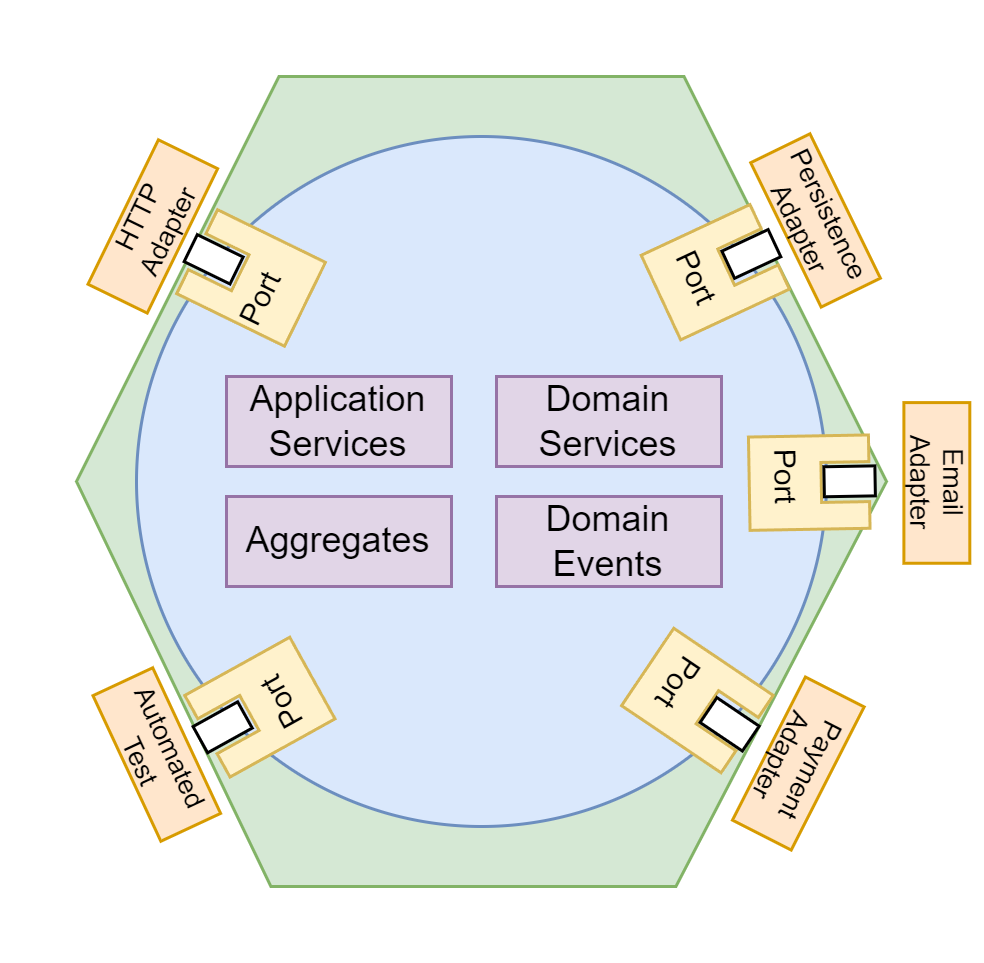
\includegraphics[width=0.75\textwidth]{media/hexagonal_architecture.png}
    \legend{Fonte: o autor}
    \label{fig:arquitetura_hexagonal}
\end{figure}

Na \autoref{fig:arquitetura_hexagonal}, pode-se observar que a injeção de agentes externos, como persistência em um banco de dados, é realizada por meio de portas definidas dentro do núcleo da aplicação. As portas, nessa arquitetura, são geralmente representadas por interfaces em linguagens orientadas a objetos. Então, um adaptador fornece uma implementação de uma tecnologia específica para a porta. Assim, implementações para tecnologias específicas são definidas em função do modelo de domínio.

Outros benefícios importantes, além do isolamento das regras de negócio, são: facilidade de testar o núcleo da aplicação com a utilização de \english{mocks} e \english{stubs}; possibilidade de utilização da mesma aplicação via interfaces de usuário, testes automatizados e \english{batches}.

Enquanto a \acrshort{ams} visa organizar um sistema como um conjunto de serviços independentes, cada um executando uma função específica, a arquitetura hexagonal concentra-se na organização interna de um serviço, propondo uma separação clara entre a lógica de negócios e as implementações técnicas, usando portas e adaptadores. Por outro lado, \acrshort{ddd} apresenta-se como uma excelente abordagem para desenvolvimento do núcleo da aplicação na arquitetura hexagonal. Assim, esses três conceitos: microsserviços, arquitetura hexagonal e \acrshort{ddd} podem ser combinados para o desenvolvimento de sistemas altamente coesos, desacoplados, escaláveis, inteligíveis e sustentáveis.






\chapter{Trabalhos Relacionados}
\label{cap:trabalhos}
Este capítulo apresenta os trabalhos relacionados ao objeto de pesquisa obtidos utilizando o protocolo descrito no \autoref{cap:metodologia}.

\section{Caracterização dos estudos}

\begin{figure}
\centering
\caption{Número de publicações ao longo dos anos}
\begin{tikzpicture}
\begin{axis}[
    width=0.8\textwidth,
    height=0.6\textwidth,
    xlabel={Ano},
    ylabel={Número de publicações},
    xtick=data, % Use data points for x-axis ticks
    xticklabel style={/pgf/number format/1000 sep=}, % Remove comma from tick labels
    ymajorgrids=true, % Show y-axis grid lines
    grid style=dashed, % Style of grid lines
    legend pos=north west, % Position of the legend
]
\addplot[
    smooth, % Show only the dots without connecting lines
    mark=*,
    mark options={scale=1.5}, % Adjust dot size
] table [x=Year, y=Publications, col sep=comma] {media/publications_per_year.csv};
\end{axis}
\end{tikzpicture}
\legend{Fonte: \english{Scopus}}
\label{fig:publications_per_year}
\end{figure}

Na \autoref{fig:publications_per_year}, pode-se observar a quantidade de publicações por ano, encontradas a partir da expressão de busca descrita na seção \ref{section:string_busca}. No total, foram obtidos 65 resultados. Percebe-se, claramente, um aumento exponencial no número de publicações sobre o tema, principalmente a partir de 2019, demonstrando crescimento no interesse de se realizar pesquisas sobre o assunto.

\begin{figure}
    \centering
    \caption{Publicações por localização}
    \pgfplotstableread[col sep=comma]{media/publications_per_territory.csv}\datatable

    \begin{tikzpicture}
        \begin{axis}[
            xbar,
            bar width=0.5cm,
            height=0.6\textwidth,
            width=0.8\textwidth,
            symbolic y coords={Alemanha, China, Áustria, Itália, Suíça, Taiwan, Estados Unidos, Indonésia, Brasil, Colômbia},
            ytick=data,
            xlabel={Publicações},
            ylabel={Localização},
            nodes near coords,
            nodes near coords align={horizontal},
            ]
            \addplot table[x=Publications, y=Territory] {\datatable};
        \end{axis}
    \end{tikzpicture}
    \legend{Fonte: \english{Scopus}}
    \label{fig:publications_per_territory}
\end{figure}

A Alemanha lidera em número de publicações, como pode ser visualizado na \autoref{fig:publications_per_territory}. Por outro lado, o Brasil só possui duas entre as sessenta e cinco publicações retornadas.

Utilizando-se os critérios de inclusão e exclusão descritos nas seções \ref{section:criterios_inclusao} e \ref{section:criterios_exclusao}, respectivamente, dos 65 artigos retornados, 27 foram selecionados inicialmente. Após realizada as leituras, apenas 16 publicações mostraram-se relevantes para responder às questões de pesquisa e/ou apoiar na elaboração do estudo de caso. Esta listagem está disponível no \autoref{quad:publicacoes_selecionadas}. 

\begin{quadro}
\centering

\setlength{\tabcolsep}{0.8em} % for the horizontal padding
\renewcommand{\arraystretch}{1.5}% for the vertical padding
\begin{tabular}{p{3in}|p{1in}|p{0.5}}
\hline

\multicolumn{1}{|p{4in}}{\textbf{Título}} & 
\multicolumn{1}{|p{0.5in}|}{\textbf{Ano}} \\
\hhline{---}

\multicolumn{1}{|p{4in}}{\english{Microservice Migration Using Strangler Fig Pattern and Domain-Driven Design}} & 
\multicolumn{1}{|p{0.5in}|}{\citeyear{ma20221285}} \\
\hhline{---}

\multicolumn{1}{|p{4in}}{\english{Microservice architecture and model-driven development: Yet singles, Soon Married ?}} & 
\multicolumn{1}{|p{0.5in}|}{\citeyear{Rademacher2018}} \\
\hhline{---}

\multicolumn{1}{|p{4in}}{\english{Does Domain-Driven Design Lead to Finding the Optimal Modularity of a Microservice?}} & 
\multicolumn{1}{|p{0.5in}|}{\citeyear{Vural202132721}} \\
\hhline{---}

\multicolumn{1}{|p{4in}}{\english{Modeling Microservices with DDD}} & 
\multicolumn{1}{|p{0.5in}|}{\citeyear{Merson20207}} \\
\hhline{---}

\multicolumn{1}{|p{4in}}{\english{Following Domain Driven Design principles for Microservices decomposition: Is it enough?}} & 
\multicolumn{1}{|p{0.5in}|}{\citeyear{Farsi2021}} \\
\hhline{---}

\multicolumn{1}{|p{4in}}{\english{An Ontology-based Approach for Domain-driven Design of Microservice Architectures}} & 
\multicolumn{1}{|p{0.5in}|}{\citeyear{Diepenbrock20171777}} \\
\hhline{---}

\multicolumn{1}{|p{4in}}{\english{Challenges of domain-driven microservice design: A model-driven perspective}} & 
\multicolumn{1}{|p{0.5in}|}{\citeyear{Rademacher201836}} \\
\hhline{---}

\multicolumn{1}{|p{4in}}{\english{Model-based engineering for microservice architectures using Enterprise Integration }} & 
\multicolumn{1}{|p{0.5in}|}{\citeyear{Petrasch2017}} \\
\hhline{---}

\multicolumn{1}{|p{4in}}{\english{Patterns on Deriving APIs and their Endpoints from Domain Models }} & 
\multicolumn{1}{|p{0.5in}|}{\citeyear{Singjai2021}} \\
\hhline{---}

\multicolumn{1}{|p{4in}}{\english{Refactoring with domain-driven design in an industrial context: An action research report}} & 
\multicolumn{1}{|p{0.5in}|}{\citeyear{Ozkan2023}} \\
\hhline{---}

\multicolumn{1}{|p{4in}}{\english{A microservice based reference architecture model in the context of enterprise architecture}} & 
\multicolumn{1}{|p{0.5in}|}{\citeyear{Yale20171856}} \\
\hhline{---}

\multicolumn{1}{|p{4in}}{\english{Design of Domain-driven Microservices-based Software Talent Evaluation and Recommendation System}} & 
\multicolumn{1}{|p{0.5in}|}{\citeyear{Zhang2022310}} \\
\hhline{---}

\multicolumn{1}{|p{4in}}{\english{Partitioning microservices: A domain engineering approach}} & 
\multicolumn{1}{|p{0.5in}|}{\citeyear{Joselyne201843}} \\
\hhline{---}

\multicolumn{1}{|p{4in}}{\english{Practitioner Views on the Interrelation of Microservice APIs and Domain-Driven Design: A Grey Literature Study Based on Grounded Theory}} & 
\multicolumn{1}{|p{0.5in}|}{\citeyear{Singjai202125}} \\
\hhline{---}

\multicolumn{1}{|p{4in}}{\english{A Systematic Framework of Application Modernization to Microservice based Architecture}} & 
\multicolumn{1}{|p{0.5in}|}{\citeyear{Joselyne2021}} \\
\hhline{---}

\multicolumn{1}{|p{4in}}{\english{Domain-specific language and tools for strategic domain-driven design, context mapping and bounded context modeling}} & 
\multicolumn{1}{|p{0.5in}|}{\citeyear{Kapferer2020299}} \\
\hhline{---}

\end{tabular}
\caption{Publicações selecionadas}
\label{quad:publicacoes_selecionadas}
\end{quadro}


\section{Estratégias para elaboração de sistemas com microsserviços e DDD}
Todas as publicações revisadas sugerem o mapeamento de cada \nameref{section:bounded_context} para um microsserviço. \citeonline{Vural202132721} afirmam que o objetivo principal da delimitação é alcançar serviços com baixo acoplamento e alta coesão. Porém, o grande desafio está na definição de maneira apropriada do escopo de cada \acrshort{bc}.

\citeonline{Singjai202125} e \citeonline{ma20221285} mencionam os padrões \english{\acrfull{ohs}} e \english{\acrfull{acl}} como estratégias para comunicação, conceitualmente, entre \hyperref[section:bounded_context]{Bounded Contexts}. No \acrshort{ohs}, o serviço que envia as mensagens implementa uma camada extra com objetivo de realizar a tradução para um formato que possa ser processado pelo serviço receptor. Dessa forma, os detalhes de implementação do serviço cliente não são expostos, diminuindo o acoplamento entre as partes. Semelhantemente, o \acrshort{acl} é uma camada extra inserida no serviço que recebe as mensagens. Trata-se de uma abordagem útil quando o serviço receptor não deseja aderir ao contrato do componente que produz as mensagens \cite{evans2004ddd}.

Outro ponto importante levantando no material revisado é o mapeamento do modelo de domínio para uma \acrfull{api} para possibilitar o consumo das funcionalidades tanto por outros serviços quanto de aplicações cliente. Algumas opções citadas por \citeonline{Singjai202125} são:
\begin{itemize}
    \item Expor todo o modelo de domínio em uma relação de 1 para 1 com a \acrshort{api}.
    \item Expor uma parte do modelo como uma \acrshort{api}.
    \item Expor cada \acrshort{bc} como uma \acrshort{api}.
    \item Expor parte dos \acrshort{bc}s como \acrshort{api}s.
\end{itemize}

As alternativas mais indicadas são a exposição total ou de grupo de \acrshort{bc}s como \acrshort{api}s. Além disso, \citeonline{Singjai202125} e \citeonline{Singjai2021} levantam abordagens para definição do contrato de \acrshort{api} de acordo com modelo de domínio. As duas principais opões apresentadas pelos autores são: explicitamente definir o contrato de \acrshort{api} e extrair o contrato de \acrshort{api} a partir do modelo. \citeonline{Singjai202125} argumenta que ambas opções auxiliam na obtenção da separação do contrato de \acrshort{api} e das responsabilidades do modelo de domínio.

Para este trabalho de conclusão de curso, a estratégia de mapeamento de um \acrshort{bc} para um microsserviço é utilizada. Com objetivo de habilitar a comunicação entre subdomínios, o padrão \acrfull{ohs} é empregado. Adicionalmente, o contrato de \acrshort{api} será definido explicitamente a partir do modelo de domínio. Assim, pretende-se utilizar as estratégias mais indicadas pelos autores revisados na elaboração do estudo de caso.

\section{Desafios na utilização de DDD como estratégia de delimitação de microsserviços}
\citeonline{Rademacher201836} menciona três principais desafios da utilização de \acrshort{ddd} no contexto da \acrshort{ams}. Adicionalmente, \citeonline{Diepenbrock20171777} cita desafios semânticos juntamente com sua proposta de metamodelo.

A ciência desse conjunto de desafios é crucial para elaboração do estudo de caso deste trabalho de conclusão de curso.

\subsection{Extraindo microsserviços a partir de modelos de domínio}
Para fomentar o foco em conceitos relevantes e \english{design} efetivo, modelos de domínio tipicamente omitem informações obrigatórias para extração de microsserviços, como:
\begin{itemize}
    \item Interfaces e operações;
    \item Parâmetros e tipos de retorno das operações
    \item \english{Endpoints}, protocolos e formatos de mensagens.
\end{itemize}
\cite{Rademacher201836}.

Informações específicas sobre esses pontos são cruciais para implementação dos serviços. Considerando diferentes \acrshort{bc}s conectados entre si no modelo, e que cada \acrshort{bc} é mapeado para um microsserviço, um componente vai necessitar acessar instâncias de um outro serviço. Assim, uma operação desse tipo deve ser fornecida e usualmente não é especificada no modelo, deixando espaço para ambiguidade \cite{Rademacher201836}.

\subsection{Componentes de infraestrutura faltantes no modelo de domínio}
Modelos de domínio intencionalmente não compreendem componentes de infraestrutura da \acrshort{ams} \cite{Rademacher201836}. Esses componentes incluem \english{API Gateways}, \english{containers}, banco de dados, entre outros. Por outro lado, requisitos do modelo podem afetar questões técnicas e esses pontos devem ser documentados separadamente do modelo de domínio \cite{Rademacher201836}. Por exemplo, caso um microsserviço que realize o gerenciamento de usuários necessite ser acessível externamente para faturamento, configurações em diferentes componentes técnicos como \english{API Gateway} necessitarão ser aplicadas.

\subsection{Modelagem de domínio autônoma}
Responsabilidade sobre um microsserviço é geralmente atribuída a um único time, devido à alta coesão e baixo acoplamento \cite{Rademacher201836}. Essa equipe é responsável pela implementação do serviço, operação, \english{design} e manutenção desse \acrfull{bc}. Dessa forma, surgem desafios relacionados a visibilidade dos modelos e gerenciamento de alterações.

Primeiramente, é crucial definir a visibilidade de cada \acrshort{bc}, ou seja, especificar quais equipes terão acesso a quais modelos de domínios \cite{Rademacher201836}. Além disso, a permissão para realizar alterações é uma consideração essencial. Embora seja possível conceder a outras equipes privilégios para modificar outros \acrshort{bc}, essa abordagem apresenta a desvantagem de possibilitar alterações, por vezes críticas, efetuadas por profissionais que não estão familiarizados com o contexto específico. No entanto, restringir exclusivamente à equipe responsável a capacidade de realizar mudanças pode resultar em gargalos significativos, especialmente em projetos envolvendo diversos contextos.

\subsection{Desafios semânticos}
\citeonline{Diepenbrock20171777} apresenta uma série de desafios semânticos na elaboração de microsserviços com \acrshort{ddd}. Inicialmente, um problema de semântico típico ocorre quando um atributo de um conceito de domínio é derivado de outro atributo. Por exemplo, quando um atributo de uma entidade é criado a partir da concatenação de dois outros atributos de outra entidade, ocorre um problema de semântica porque os dados ficam fragmentados.

Simultaneamente, é importante reconhecer que diferentes \acrshort{bc}s podem interpretar os conceitos de domínio compartilhados de maneiras distintas \cite{Diepenbrock20171777}. Nesse contexto, surgem desafios como atributos com nomes diversos, mas significados idênticos, bem como propriedades com o mesmo nome, porém, com significados diferentes. Esse risco é amplificado no contexto da \acrshort{ams}, onde é comum que diferentes \acrshort{bc}s sejam desenvolvidos por equipes distintas. Esse ambiente descentralizado pode potencializar a disparidade de interpretações e a falta de consistência nos conceitos de modelos compartilhados.

Além disso, um mecanismo de definição de identificadores únicos deve ser definido entre as equipes para permitir a identificação semântica de diferentes conceitos do modelo com objetivo de tornar os serviços capazes de distinguir diferentes elementos em um contexto distribuído \cite{Diepenbrock20171777}.

Por essas motivações, \citeonline{Diepenbrock20171777} apresenta uma abordagem para \acrshort{ddd} no contexto da \acrshort{ams}. O autor propõe um metamodelo que representa a sintaxe abstrata de um linguagem formal de modelagem. Em outras palavras, ele define os conceitos suportados pela linguagem e seus relacionamentos. Os principais componentes do metamodelo são: \english{External Context}, \english{\acrlong{bc}}, \english{Domain Model}, \english{Attribute} e \english{Association}. O objetivo principal desse modelo é minimizar os impactos dos desafios semânticos da utilização dessas tecnologias \cite{Diepenbrock20171777}.

\section{Anti-padrões a serem evitados}
\citeonline{Farsi2021}, \citeonline{Vural202132721}, \citeonline{Singjai2021}, \citeonline{Ozkan2023} e \citeonline{Singjai202125} identificaram uma série de anti-padrões no contexto da \acrshort{ams} e \acrshort{ddd}. Um compilado pode ser observado no \autoref{quad:anti_padroes}.

\begin{quadro}
\centering
\caption{Anti-padrões}
\setlength{\tabcolsep}{0.8em} % for the horizontal padding
\renewcommand{\arraystretch}{1.5}% for the vertical padding
\begin{tabular}{|p{1in}|p{3.7in}|}
\hline

\textbf{Nome} & \textbf{Descrição} \\ \hline
\english{Chattiness of a service} &  Refere-se a excessiva comunicação entre microsserviços que gera ineficiência devido à latência de rede. \\ \hline
\english{Nanoservice} & Um serviço excessivamente granular no qual a sobrecarga de comunicação, manutenção e operação supera sua utilidade. \\ \hline
\english{Anemic domain model} & Trata-se de um modelo de domínio em que os objetos contém pouca ou nenhuma regra de negócio. As invariantes são misturadas com outras lógicas, o que dificulta manutenção e refatoração. \\ \hline
\english{Data class} & Similar ao \english{Anemic domain model}, esse tipo de classe só contem, além de atributos, \english{getters} e \english{setters}. Os comportamentos são criados fora da classe, o que reduz coesão e dificulta a manutenção. \\ \hline
\english{Distributed monoliths} & Refere-se a um sistema que externamente se assemelha a \acrlong{ams}, porém possui um alto nível de acoplamento entre os componentes, diminuindo assim as vantagens dos microsserviços. \\ \hline
\english{Start with API Design} & Trata-se de uma abordagem na qual o contrato de \acrshort{api} é definido antes do modelo de domínio. \citeonline{Singjai2021} levantou que esta estratégia costuma gerar a criação de \english{Anemic domain models}. \\ \hline
\english{Feature envy} & Acontece quando um método está mais interessado em uma classe diferente da que está inserido. \\ \hline
\english{Inappropiate intimacy} & Descreve um par de classes não relacionadas conceitualmente, mas que possuem grande acoplamento entre si. \\ \hline
\english{Message chain} & Uma cadeia de mensagem ocorre quando um cliente envia uma mensagem a outro objeto que, por sua vez, a envia outro o objeto e assim por diante. \\ \hline

\end{tabular}
\fonte{\citeonline{Farsi2021}, \citeonline{Vural202132721}, \citeonline{Singjai2021}, \citeonline{Ozkan2023} e \citeonline{Singjai202125}}
\label{quad:anti_padroes}
\end{quadro}

Os anti-padrões mencionados são importantes para o desenvolvimento do estudo de caso, pois devem ser evitados para que os benefícios da utilização conjunta de \acrshort{ddd} e \acrshort{ams} sejam alcançados.

\section{Discussões}
O mapeamento da literatura mostrou-se efetivo para responder às questões de pesquisa, na medida em que foram encontradas publicações que auxiliam na resolução das perguntas-chave. O levantamento das estratégias, desafios e anti-padrões foi realizado com êxito a partir de artigos de alta qualidade.

No entanto, publicações em outros idiomas que não foram revisadas, assim como publicações não indexadas pelas ferramentas de busca utilizadas, representam uma ameaça a validade da pesquisa. Isso se deve ao fato de que informações essenciais podem não ter sido revisadas devido a essas limitações

Por fim, as informações obtidas nesse mapeamento contribuem tanto para atingir os objetivos gerais da pesquisa quanto para a elaboração do estudo de caso.


\chapter{Metodologia}
\label{cap:metodologia}
Este capítulo apresenta a metodologia e os recursos utilizados para atingir o objetivo do trabalho.

\section{Visão geral}
\begin{figure}[h]
    \centering
    \caption{Etapas de desenvolvimento da pesquisa}
    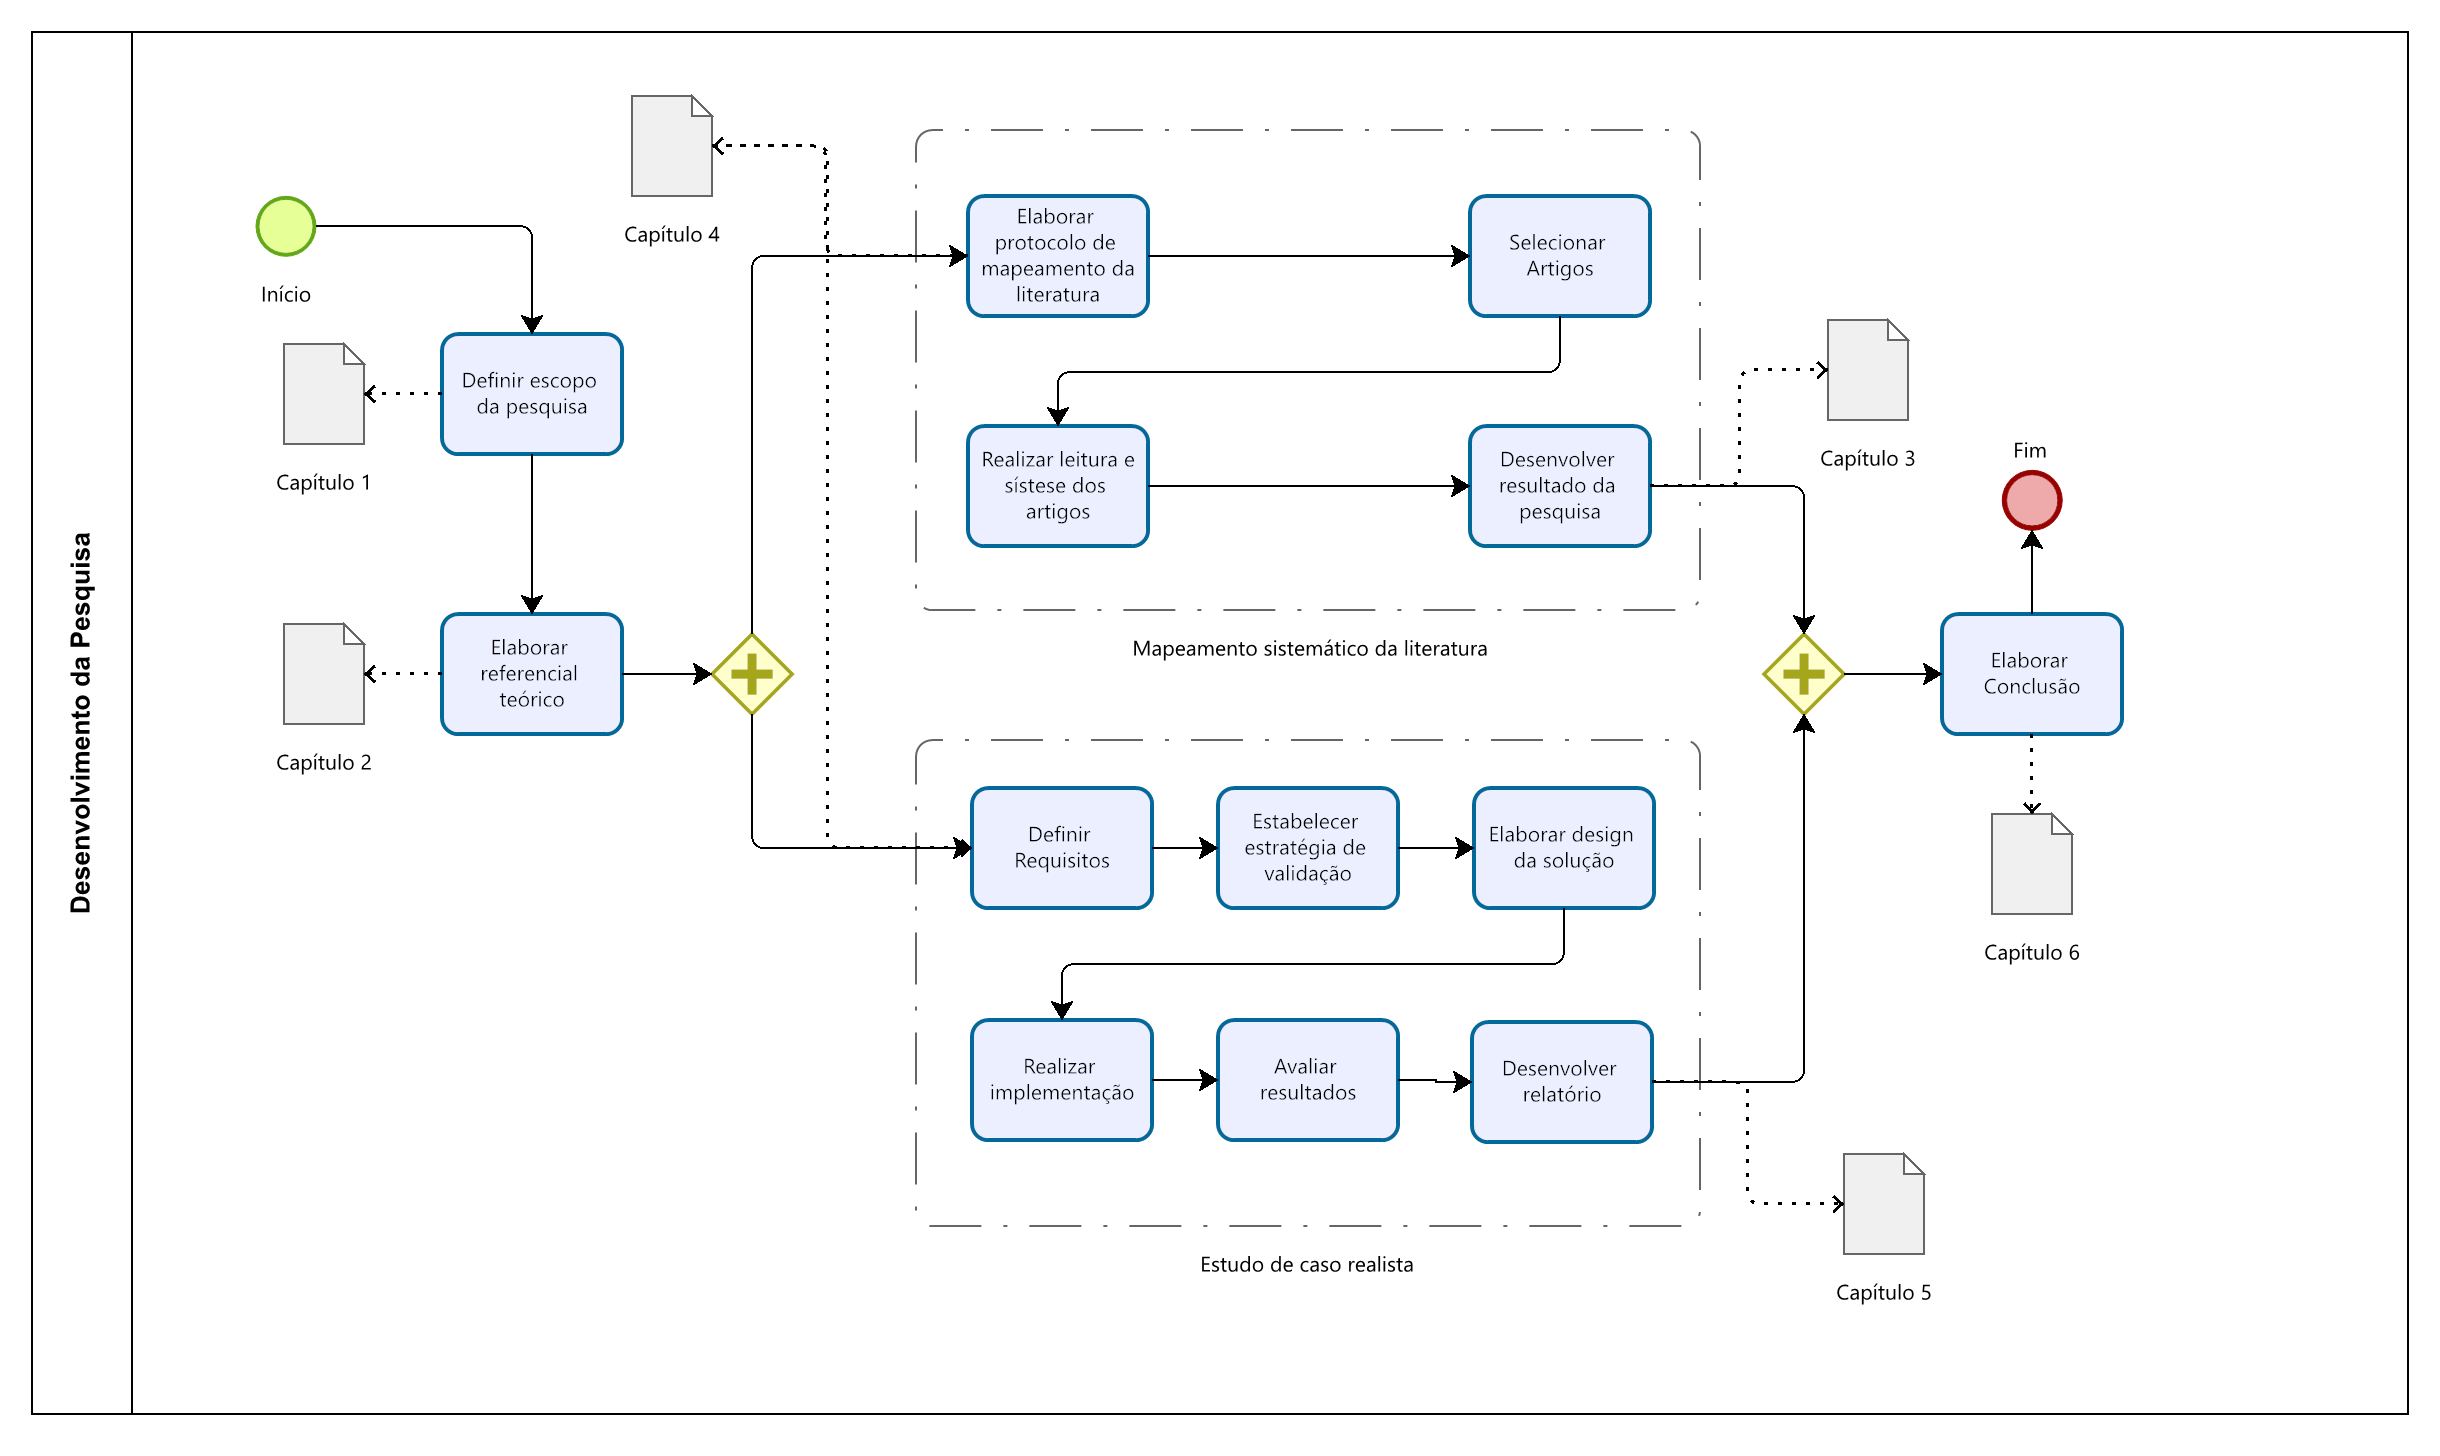
\includegraphics[width=0.9\textwidth]{media/bpmn_metodo_recurso.png}
    \legend{Fonte: o autor}
    \label{fig:metodo_recurso}
\end{figure}

Pode-se observar na \autoref{fig:metodo_recurso} as etapas de execução dessa pesquisa. Inicialmente, o escopo é definido e o primeiro capítulo é elaborado. Em seguida, a fundamentação teórica com os conceitos-chave é construída. Posteriormente, se realiza um mapeamento da literatura buscando trabalhos similares. Paralelamente a isso, um estudo de caso realista com a utilização de microsserviços e diversos conceitos do \acrshort{ddd} é desenvolvido e um relatório é produzido. Por fim, é escrita a conclusão do trabalho.

\section{Mapeamento sistemático da Literatura}
Esta seção apresenta o protocolo de mapeamento sistemático da literatura usado para atingir os objetivos da pesquisa.

\subsection{Questões de pesquisa}
\label{section:questoes_pesquisa}
\begin{enumerate}
    \item[Q1:] Quais são as principais estratégias para elaboração de sistemas com microsserviços e \acrshort{ddd}?
    \item[Q2:] Quais são os principais desafios na utilização de \acrshort{ddd} como estratégia de delimitação de microsserviços?
    \item[Q2:] Quais são os anti-padrões a serem evitados na utilização de \acrshort{ddd} com microsserviços?
    
\end{enumerate}

\subsection{Estratégia de busca}
Esta seção apresenta a estratégia de buscas de artigos científicos e livros relacionados à pesquisa. As ferramentas utilizadas para realizar as buscas são:
\begin{itemize}
    \item \textbf{Periódicos Capes:} É uma ferramenta disponibilizada pelo governo federal para uso de estudantes e pesquisadores. Acessando através da instituição de ensino ou pesquisa, é possível ter acesso completo a uma grande quantidade de artigos científicos publicados em variadas revistas, conferências e universidades. A principal vantagem dessa ferramenta é a possibilidade de ler o conteúdo integral de grande parte das publicações disponíveis. Por outro lado, as expressões de busca atualmente suportadas são bem limitadas.
    \item \textbf{\english{Scopus:}} Trata-se de um ferramenta similar ao Periódicos Capes. No entanto, o \english{Scopus} permite a elaboração de expressões de buscas mais complexas e sofisticadas, servindo para descobrir publicações não detectadas pelas outras plataformas. Além disso, possui um acervo bem mais amplo que o Periódicos Capes. Entretanto, algumas publicações não podem ser vistas na íntegra de forma gratuita.
    \item \textbf{\english{Google Docs:}} Ferramenta desenvolvida pela \english{Google LLC} que permite a criação e edição de documentos de texto. Suas grandes vantagens em relação a ferramentas de outros fornecedores são as avançadas ferramentas de colaboração e a possibilidade de acesso por meio de navegadores \english{web}, sem necessidade de instalação de \english{software} específico.
    \item \textbf{\english{Google Sheets}}: Com as mesmas características e vantagens do \english{Google Docs}, essa ferramenta fornece recursos para elaboração de planilhas de cálculo. É muito útil para realizar análise de dados simples e também visualizar e apresentar dados tabulares.
\end{itemize}

Como grande parte das publicações na área de computação são em inglês, esta pesquisa utiliza esse idioma para fazer buscas nas ferramentas indicadas. Além disso, \acrfull{ams} e \acrfull{ddd} são relativamente recentes, as buscas se limitaram a publicações feitas nos últimos 20 anos.

Os termos-chave para realização das buscas são: Microsserviço, \acrshort{ddd} e \acrlong{ddd}. Como a busca é feita em inglês, se usará \english{microservice} nas buscas.
\subsection{Expressão de busca}
\label{section:string_busca}

\begin{quadro}[H]
\centering

\setlength{\tabcolsep}{0.8em} % for the horizontal padding
\renewcommand{\arraystretch}{1.5}% for the vertical padding
\caption{Expressão de busca utilizada}
\begin{tabular}{|p{4.5in}|}

\hline
Expressão de Busca \\ \hline
\english{( ( TITLE-ABS-KEY ( microservice ) AND TITLE-ABS-KEY ( domain-driven AND design ) ) OR ( TITLE-ABS-KEY ( microservice ) AND TITLE-ABS-KEY ( ddd ) ) )} \\ \hline

\end{tabular}
\label{quad:string_busca}
\fonte{o autor}
\end{quadro}

No \autoref{quad:string_busca}, percebe-se que a expressão de busca pretende retornar todas as publicações que contenham as palavras chaves no título, resumo ou na seção de \english{keywords}.

\subsection{Estratégia de seleção}
A seguir são apresentados critérios para inclusão de publicações na pesquisa.
\label{section:criterios_inclusao}
\begin{itemize}
    \item Texto completo disponível de forma gratuita pelo portal Periódicos Capes.
    \item Materiais relacionados ao tópico de interesse, ou seja, título ou resumo.
    \item Publicações com ao menos 5 citações.
\end{itemize}

Por outro lado, estes são os critérios para exclusão de publicações.
\label{section:criterios_exclusao}
\begin{itemize}
    \item Publicações duplicadas.
    \item Materiais que não dispõem de informação relevante para responder às questões de pesquisa.
\end{itemize}

\subsection{Estratégia para extração de dados e análise}
Para atingir o objetivo do mapeamento da literatura, são filtrados manualmente nos artigos selecionados segundo os critérios de inclusão e exclusão. A partir da listagem reduzida, todas as publicações são lidas de forma integral.
Adicionalmente, todos os gráficos e tabelas nos artigos selecionados são avaliados visando extrair algum dado que permita realizar a comparação entre aspectos quantitativos das estratégias como, tempo de resposta, latência e taxa de transferência.

Informações qualitativas como recomendações, destaques, conceitos e estudos de casos são registrados em um documento no \english{\href{https://docs.google.com/document/d/1-dXE9_2-CtfDePG9Opkcyipq0F0dcYJ-Z_gbhi_qDhs/edit?usp=sharing}{Google Docs}}. Dados quantitativos como taxa de transferência, latência, tempo de processamento são armazenados em uma planilha no \english{\href{https://docs.google.com/spreadsheets/d/1R-PbCisie8QHARzF2rYtDx8UPOWksEeH-6-SEqIOTLg/edit?usp=sharing}{Google Sheets}}. 

A pesquisa é executada seguindo os passos a seguir:
\begin{enumerate}
    \item As expressões de busca citadas são inseridas nas ferramentas mencionadas.
    \item É feito o armazenamento das publicações retornadas em uma \href{https://docs.google.com/spreadsheets/d/1rtH8Jl1EHguqZ4Py2mgV3pab7IQzt72-Sv2S1jPzLsQ/edit?usp=sharing}{planilha de cálculo}.
    \item As publicações retornadas são filtradas conforme os critérios de inclusão e exclusão.
    \item Em cada artigo selecionado, é realizada a extração dos dados relevantes para responder às questões de pesquisa.
    \item Finalmente, são produzidas respostas para questões de pequisa com as informações extraídas das publicações.
\end{enumerate}

\section{Estudo de Caso}

\subsection{Contexto}
\label{section:contexto}
O estudo de caso é realizado em uma empresa fictícia chamada \emph{CarroFacil}. Essa empresa é uma locadora de veículos que atua em todo o território nacional. Ela possui uma frota de veículos própria e uma grande quantidade de clientes. Eles podem alugar veículos por períodos de tempo variados, desde horas até semanas. A \emph{CarroFacil} possui um sistema de locação de veículos que foi desenvolvido há alguns anos e está apresentando problemas de escalabilidade, desempenho e manutenibilidade. Por esse motivo, a empresa decidiu desenvolver um novo sistema de locação de veículos utilizando microsserviços e \acrshort{ddd}.

\begin{figure}[!h]
    \centering
    \caption{Diagrama de caso de uso}
    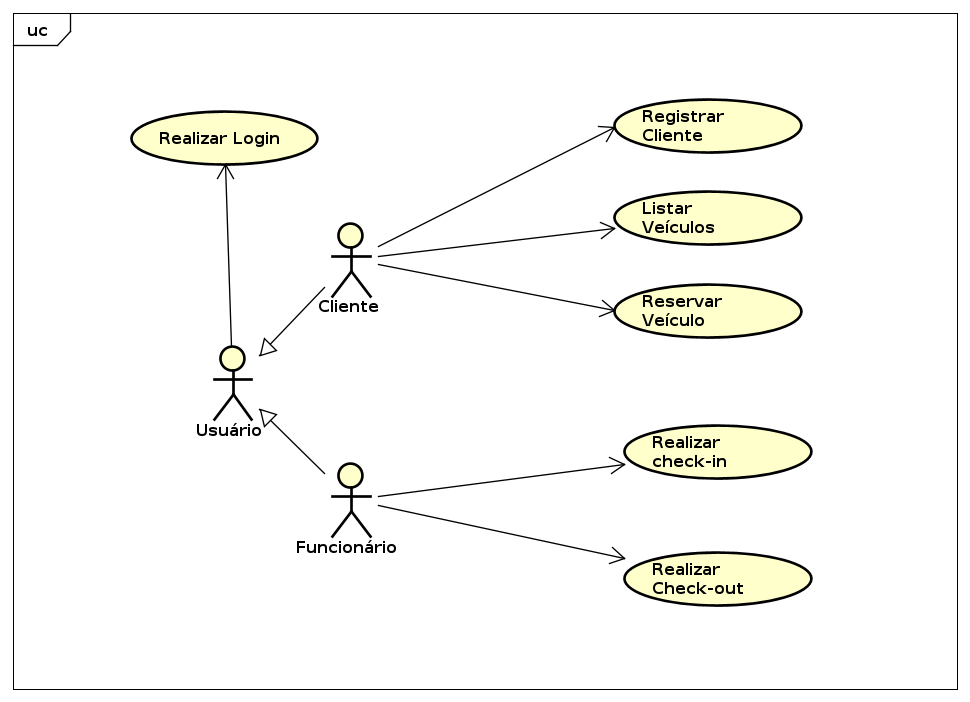
\includegraphics[width=0.9\textwidth]{media/diagrama_usecase.png}
    \legend{Fonte: o autor}
    \label{fig:caso_uso}
\end{figure}

A \autoref{fig:caso_uso} apresenta o diagrama de caso de uso do sistema de locação de veículos. As seções a seguir apresentam um detalhamento dos casos de uso do sistema.

\subsection{Processo de Desenvolvimento}
\label{section:processo_desenvolvimento}
O processo de desenvolvimento utilizado para construir o sistema de locação de veículos é o \english{Kanban}. Essa metodologia de desenvolvimento ágil é baseada em um quadro de tarefas, no qual cada tarefa é representada por um cartão \cite{gomes2014agile}. O quadro é dividido em colunas que representam o estado atual de cada tarefa. As colunas mais comuns são: \english{To Do}, \english{Doing} e \english{Done}. O quadro é atualizado conforme as tarefas são realizadas. A \autoref{fig:kanban} apresenta um exemplo de quadro \english{Kanban} que é utilizado para mapear as tarefas e medir o progresso do desenvolvimento deste sistema.

\begin{figure}[ht!]
    \centering
    \caption{Exemplo de quadro \english{Kanban}}
    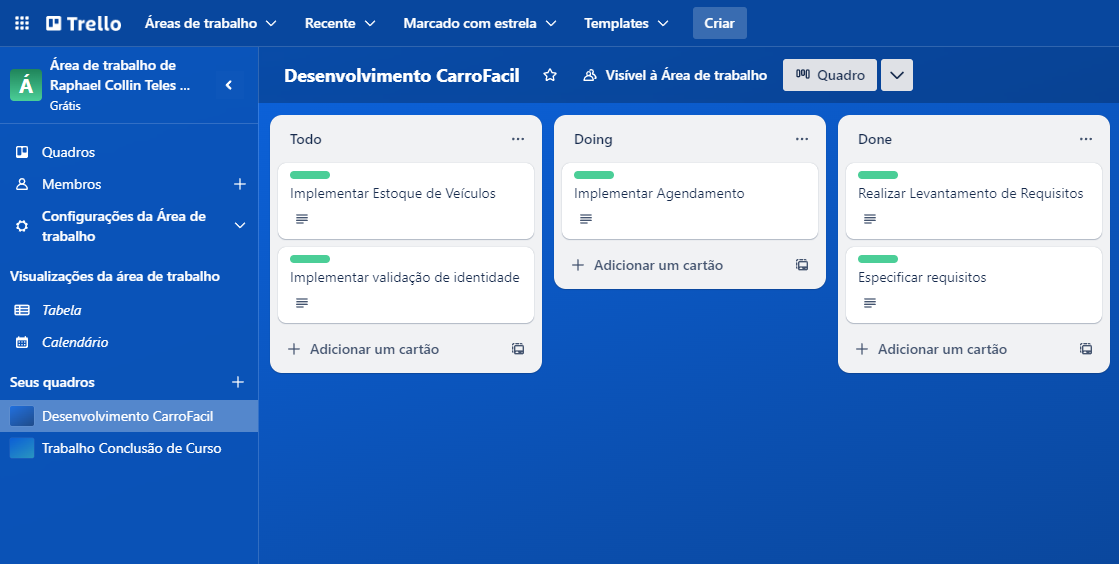
\includegraphics[width=0.9\textwidth]{media/kanban.png}
    \legend{Fonte: o autor}
    \label{fig:kanban}
\end{figure}

\subsection{Requisitos}
A seguir são apresentados os requisitos do sistema de locação de veículos.
\subsubsection{Requisitos Funcionais}

\begin{quadro}[H]
    \centering
    \caption{Registrar cliente}
    \label{quad:registrar_cliente}
    \begin{tabular}{|p{1.2in}|p{3.5in}|}
    \hline
    
    \textbf{Caso de uso} & Registrar cliente \\ \hline
    \textbf{Descrição} & Permite que o cliente se cadastre na plataforma. \\ \hline
    \textbf{Ator} & Cliente \\ \hline
    \textbf{Pre-condições} & O cliente ainda não está cadastrado. \\ \hline
    \textbf{Pós-condições} & O cliente é registrado na plataforma.\\ \hline
    \textbf{Cenário Principal} & \begin{enumerate}
        \item O cliente informa o nome, e-mail e senha.
        \item O cliente recebe uma confirmação do cadastro.
    \end{enumerate}  \\ \hline
    \textbf{Fluxo de Exceção} & \begin{enumerate}
        \item Dados inválidos são informados. Nesse caso, o sistema exibe uma mensagem de erro.
        \item Usuário já cadastrado. O sistema também exibe uma mensagem de erro customizada para esse caso.
    \end{enumerate}  \\ \hline
    \end{tabular}
    \fonte{o autor.}
\end{quadro}

O caso de uso do \autoref{quad:registrar_cliente} especifica o registro de um cliente. Esse é o primeiro passo para que um cliente possa realizar uma reserva de veículo.

\begin{quadro}[H]
    \centering
    \caption{Listar veículos}
    \label{quad:listar_veiculos}
    \begin{tabular}{|p{1.2in}|p{3.5in}|}
    \hline
    
    \textbf{Caso de uso} & Listar veículos \\ \hline
    \textbf{Descrição} & Permite que o cliente visualize os veículos disponíveis para locação. \\ \hline
    \textbf{Ator} & Cliente \\ \hline
    \textbf{Pre-condições} & O cliente está autenticado na plataforma. \\ \hline
    \textbf{Pós-condições} & Uma listagem de veículos disponíveis é exibida. \\ \hline
    \textbf{Cenário Principal} & O cliente acessa a página de veículos, onde é possível visualizar os veículos disponíveis. \\ \hline
    
    \end{tabular}
    \fonte{o autor.}
\end{quadro}

O \autoref{quad:listar_veiculos} especifica o processo de listagem de veículos. Esse processo é realizado pelo cliente e permite que ele visualize os veículos disponíveis para aluguel.

\begin{quadro}[H]
    \centering
    \caption{Reservar um veículo}
    \label{quad:reservar_veiculo}
    \begin{tabular}{|p{1.2in}|p{3.5in}|}
    \hline
    
    \textbf{Caso de uso} & Reservar um veículo \\ \hline
    \textbf{Descrição} & Permite que um cliente reserve um veículo por um período de tempo. \\ \hline
    \textbf{Ator} & Cliente \\ \hline
    \textbf{Pre-condições} & O cliente está autenticado na plataforma. \\ \hline
    \textbf{Pós-condições} & Veículo reservado fica indisponível para outros clientes. \\ \hline
    \textbf{Cenário Principal} & \begin{enumerate}
        \item O usuário seleciona o veículo, a data de início e a data de término da locação.
        \item É exibida uma confirmação para o usuário.
    \end{enumerate}  \\ \hline
    \textbf{Fluxo de Exceção} & \begin{enumerate}
        \item O veículo não está mais disponível.
        \item O cliente seleciona um período de tempo indisponível.  
        \item Em ambos os casos, o cliente é alertado sobre o problema.
    \end{enumerate}  \\ \hline
    \end{tabular} 
    \fonte{o autor.}
\end{quadro}

O \autoref{quad:reservar_veiculo} especifica o processo de reserva de um veículo. Esse processo é realizado pelo cliente e permite que ele alugue um veículo por um período de tempo.

\begin{quadro}[H]
    \centering
    \caption{Realizar \english{check-in}}
    \label{quad:realizar_checkin}
    \begin{tabular}{|p{1.2in}|p{3.5in}|}
    \hline
    
    \textbf{Caso de uso} & Realizar \english{check-in} \\ \hline
    \textbf{Descrição} & Permite a realização do check-in da reserva entre o cliente e o funcionário. \\ \hline
    \textbf{Ator} & Funcionário \\ \hline
    \textbf{Pre-condições} & \begin{enumerate}
        \item \O cliente está autenticado na plataforma.
        \item O cliente possui uma reserva criada e seu identificador.
    \end{enumerate} \\ \hline
    \textbf{Pós-condições} & O status da reserva é alterado para em progresso. \\ \hline
    \textbf{Cenário Principal} & O cliente apresenta o identificador da reserva ao funcionário que o insere no sistema para realizar o check-in. \\ \hline
    \textbf{Fluxo de Exceção} & \begin{enumerate}
        \item O check-in para aquela reserva já foi realizado.
        \item O usuário é alertado sobre o problema.
    \end{enumerate}  \\ \hline
    \end{tabular}
    \fonte{o autor.}
\end{quadro}

O caso de uso Realizar \english{check-in} é apresentado no \autoref{quad:realizar_checkin}. Esse caso de uso é realizado pelo funcionário e permite que o cliente retire o veículo reservado.

\begin{quadro}[H]
    \centering
    \caption{Realizar \english{check-out}}
    \label{quad:realizar_checkout}
    \begin{tabular}{|p{1.2in}|p{3.5in}|}
    \hline
    
    \textbf{Caso de uso} & Realizar \english{check-out} \\ \hline
    \textbf{Descrição} & Permite a realização do check-out da reserva entre o cliente e o funcionário. \\ \hline
    \textbf{Ator} & Funcionário \\ \hline
    \textbf{Pre-condições} & \begin{enumerate}
        \item O cliente possui uma reserva em progresso e seu identificador.
        \item O cliente está autenticado na plataforma.
    \end{enumerate} \\ \hline
    \textbf{Pós-condições} & O status da reserva é alterado para concluída. \\ \hline
    \textbf{Cenário Principal} & O cliente retorna o veículo, o funcionário verifica o estado do veículo, e obtém informações sobre a reserva a partir da placa. Por fim, o funcionário finaliza a reserva. \\ \hline
    \textbf{Fluxo de Exceção} & \begin{enumerate}
        \item O \english{check-in} não foi realizado para reserva.
        \item O usuário é alertado sobre o problema.
    \end{enumerate} \\ \hline
    \end{tabular}
    \fonte{o autor.}
\end{quadro}

O \autoref{quad:realizar_checkout} especifica o processo de realização do \english{check-out}. Esse processo é realizado pelo funcionário e permite que o cliente devolva o veículo alugado.

\begin{quadro}[H]
    \centering
    \caption{Listar reservas}
    \label{quad:listar_reservas}
    \begin{tabular}{|p{1.2in}|p{3.5in}|}
    \hline
    
    \textbf{Caso de uso} & Listar reservas \\ \hline
    \textbf{Descrição} & Permite que um cliente visualize as reservas que realizou. \\ \hline
    \textbf{Ator} & Cliente \\ \hline
    \textbf{Pre-condições} & Cliente está autenticado na plataforma. \\ \hline
    \textbf{Pós-condições} & Uma listagem de reservas é exibida. \\ \hline
    \textbf{Cenário Principal} & O cliente acessa a página de reservas, onde é possível visualizar as reservas realizadas. \\ \hline
    
    \end{tabular}
    \fonte{o autor.}
\end{quadro}

O \autoref{quad:listar_reservas} especifica o processo de listagem de reservas. Esse processo é realizado pelo cliente e permite que ele visualize as reservas que realizou.

\begin{quadro}[H]
    \centering
    \caption{Registrar veículo}
    \label{quad:registrar_veiculo}
    \begin{tabular}{|p{1.2in}|p{3.5in}|}
    \hline
    
    \textbf{Caso de uso} & Registrar veículo \\ \hline
    \textbf{Descrição} & Permite que um funcionário registre um novo veículo na plataforma. \\ \hline
    \textbf{Ator} & Funcionário \\ \hline
    \textbf{Pre-condições} & O funcionário está autenticado. \\ \hline
    \textbf{Pós-condições} & O veículo é registrado na plataforma. \\ \hline
    \textbf{Cenário Principal} & \begin{enumerate}
        \item O funcionário informa o tipo, marca, modelo, kilometragem, ano, placa, chassis e a cor do veículo.
        \item O funcionário envia a requisição.
    \end{enumerate}  \\ \hline
    \textbf{Fluxo de Exceção} & \begin{enumerate}
        \item Dados inválidos são informados. Nesse caso, o sistema exibe uma mensagem de erro.
    \end{enumerate}  \\ \hline
    \end{tabular}
    \fonte{o autor.}
\end{quadro}

O \autoref{quad:registrar_veiculo} especifica o processo de registro de um veículo. Esse processo é realizado pelo funcionário e permite que ele registre um novo veículo na plataforma.

\subsubsection{Requisitos não Funcionais}
Com base na quantidade de clientes atuais e a estimativa de crescimento, bem como suas expectativas quanto ao desempenho do sistema, são definidos os seguintes requisitos não funcionais:
\begin{enumerate}
    \item Os serviços devem garantir a segurança dos dados dos clientes.
    \item O tempo de resposta dos serviços deve ser menor que 2 segundos em 90\% das requisições.
    \item O sistema como um topo deve suportar 100 usuários simultâneos.
    \item As funcionalidades dos serviços devem ser fornecidadas através de \acrshort{api}s acessíveis com o protocolo HTTP.
\end{enumerate}

\subsection{Design}
Para construção de cada microsserviços, é feito uso da \hyperref[section:hexagonal]{Arquitetura Hexagonal}. Essa, por sua vez, separa a aplicação em duas partes principais: núcleo da aplicação e adaptadores. O núcleo da aplicação contém as regras de negócio e os adaptadores são responsáveis por adaptar a aplicação para o mundo externo. Para modelagem do domínio, é utilizado o \english{\acrfull{ddd}}. O \acrshort{ddd} fornece uma estratégia para modelagem do domínio de negócio, diversos padrões para resolver problemas de modelagem recorrentes e facilidade de entendimento e manutenção de código \cite{evans2004ddd}.

Para realização do \english{design} deste projeto, é utilizado a \english{UML}. Especificamente, são criados diagramas de classes com propósito de modelar os tipos de objeto, seus relacionamentos e os serviços que fornecem. Adicionalmente, para detalhamento do fluxo de execução de operações chaves, alguns diagramas de sequência são empregados. Além disso, visando fornecer uma visão geral da arquiteura do sistema, o diagrama de contexto de sistema do modelo C4 é utilizado \cite{c4Model}. 

\subsection{Implementação}
A implementação desse projeto é feita utilizando a linguagem de programação \english{Java} na versão 17 \cite{java}. Além disso, o \english{framework} \english{Spring Boot} é empregado na construção dos microsserviços. Essa ferramenta fornece uma série de recursos para construção de microsserviços como: injeção de dependências, configuração de banco de dados, configuração de \english{logs}, entre outros \cite{springBoot}. 

São utilizados dois banco de dados para armazenamento dos dados do sistema. O primeiro é um banco de dados relacional, que armazena dados de reservas e veículos. O segundo é um banco de dados não relacional, que armazena dados de usuários. Para o banco de dados relacional, é utilizado o \english{PostgreSQL} \cite{postgreSql}. Para o banco de dados não relacional, foi escolhido o \english{Amazon DynamoDB} \cite{dynamoDb}.

O \english{PostgreSQL} é um sistema de gerenciamento de banco de dados relacional de código aberto. Esse banco de dados é um dos mais populares do mundo, sendo utilizado por diversas empresas, como: \english{Apple}, \english{Spotify}, \english{Netflix}, entre outras \cite{postgreSql}. Trata-se de um banco de dados escalável, confiável, fácil de usar e com suporte a transações \acrshort{acid}.

Por outro lado, o \english{Amazon DynamoDB} é um banco de dados não relacional, que fornece desempenho de milissegundos de um dígito a qualquer escala. Esse banco de dados é totalmente gerenciado, ou seja, não é necessário realizar a configuração de servidores, escalabilidade, replicação, entre outros. Além disso, o \english{Amazon DynamoDB} é um banco de dados sem servidor, ou seja, o usuário paga apenas pelo que utiliza \cite{dynamoDb}.

Para a intercomunicação entre os microsserviços de maneira assíncrona, são utilizados o \english{Amazon Simple Notification System (SNS)} e o \english{Amazon Simple Queue System (SQS)}. O SNS é um serviço de mensagens que permite a publicação e a entrega de mensagens para assinantes ou pontos de extremidade \cite{amazonSns}. Por outro lado, o SQS é um \english{broker} permite que os microsserviços se comuniquem de maneira assíncrona, sem que um microsserviço precise conhecer o outro \cite{amazonSqs}. Além disso, o \english{Amazon SQS} permite que as mensagens sejam armazenadas em uma fila, caso o microsserviço destinatário da mensagem esteja fora do ar. Utilizados em conjunto, essas fermamentas permitem a comunicação assíncrona na forma "um para muitos" entre os microsserviços. Um microsserviço publica uma mensagem em  um tópico do SNS e os microsserviços interessados utilizam uma fila do SQS para consumir essa mensagem.

\subsection{Validação}
O projeto é desenvolvido com as estratégias \acrfull{tdd} e \acrfull{bdd}. Essas abordagens de desenvolvimento de \english{software} permitem que o código seja desenvolvido de maneira mais confiável e com maior qualidade \cite{barauna2020tdd}. Além disso, o \acrshort{tdd} e o \acrshort{bdd} permitem que o código seja desenvolvido de maneira mais rápida, pois os testes são escritos antes do código.

Três tipos de testes são escritos para validar os requisitos funcionais do sistema: testes unitários, testes de integração e testes de aceitação. Os testes unitários são escritos para validar métodos e classes do sistema. Por outro lado, os testes de integração validam a integração entre dois microsserviços e integrações com componentes externos, como banco de dados. Por fim, os testes de aceitação são implementados para validar os requisitos do sistema. É importante ressaltar que todos os testes são automatizados utilizando o \english{JUnit} \cite{junit}.

Por outro lado, para validação dos requisitos não funcionais, testes de carga são empregados. O ambiente de execução desses testes é o mesmo de implantação, definido na seção \ref{section:implantacao}. Através da ferramenta Gatling \cite{gatling}, a bateria de testes consiste de 100 usuários executando operações simultâneas por um período de 30 minutos. São avaliados o tempo de resposta, a utilização da CPU, o consumo de memória e a quantidade erros. Os resultados obtidos são comparados com o \autoref{quad:metricas_comparacao}. Cada operação possui as seguintes etapas: registrar um novo veículo, cadastrar um cliente, realizar uma reserva, realizar o \english{check-in} e realizar o \english{check-out}.

Após a execução dos testes de carga, os resultados obtidos são analizados e comparados com os requisitos não funcionais. Dessa forma, um relatório é produzido com uma análise gráfica e númerica.

\begin{quadro}[H]
    \centering
    \caption{Métricas de comparação}
    \label{quad:metricas_comparacao}
    \begin{tabular}{|p{1.2in}|p{3.5in}|}
    \hline
    
    \textbf{Métrica} & \textbf{Alvo} \\ \hline
    Tempo de resposta & <= 2 s em 90\% das requisições. \\ \hline
    Utilização da CPU & <= 70\% durante toda a execução. \\ \hline
    Consumo de memória & <= 70\% durante toda a execução. \\ \hline
    Quantidade de erros & <= 1\% das requisições. \\ \hline

    \end{tabular}
    \fonte{o autor.}
\end{quadro}

Os parâmetros descritos no \autoref{quad:metricas_comparacao} foram definidos pelo autor com base em experiências anteriores de desenvolvimento de sistemas similares no ambiente corporativo, juntamente com a recomendação do orientador.

\subsection{Implantação}
\label{section:implantacao}
O sistema é implantado na nuvem da \english{\acrfull{aws}}. A \acrshort{aws} é uma plataforma de computação em nuvem que oferece mais de 200 serviços completos de \english{data centers} em todo o mundo \cite{aws}. Esses serviços incluem computação, armazenamento, banco de dados, \english{networking}, \english{analytics}, \english{machine learning}, inteligência artificial, \english{Internet of Things}, segurança, entre outros.

Cada microsserviço é implantado em um \english{container} \english{Docker}. Essa tecnologia permite que os microsserviços sejam executados de maneira isolada, sem que um microsserviço interfira no outro. Além disso, o \english{Docker} permite que os microsserviços sejam executados em qualquer ambiente, sem que seja necessário realizar alterações no código \cite{docker}. O serviço \english{Amazon ECS} é utilizado para orquestrar os \english{containers} \english{Docker}. Esse serviço permite que os \english{containers} sejam executados em um ambiente de produção de maneira escalável e confiável \cite{amazonEcs}. Ao todo, serão utilizados 3 \english{tasks}: uma para o microsserviço de usuários, uma para o de estoque o outra para o de reservas. Cada \english{task} possui 2 CPUs e 4 GB de memória RAM.

Dois \english{clusters} do \english{PostgreSQL} com o auxílio do serviço \english{Amazon RDS} são utilizados \cite{postgreSql}. Um para o serviço de estoque e outro para o serviço de reservas. Com a arquitetura de microsserviços, é essencial o isolamento das bases de bados. Além disso, uma tabela do \english{Amazon DynamoDB} é utilizada para armazenamento de informações de usuários. Da mesma forma, um tópico do SNS para reservas e um fila SQS que consome informações de reservas e mantem um contador de reservas por usuário são utilizados.

Para a orquestração e automatização do provisionamento e configuração da infraestrutura, é feito uso da ferramenta \english{Terraform}. Essa ferramenta permite que a infraestrutura seja definida como código, ou seja, é possível definir a infraestrutura utilizando uma linguagem de programação \cite{terraform}. Além disso, o \english{Terraform} permite que a infraestrutura seja provisionada e configurada de maneira automatizada.


\chapter{Desenvolvimento}
\label{cap:desenvolvimento}

Este capítulo apresenta o desenvolvimento do estudo de caso com Microsserviços e \acrshort{ddd}. Ele descreve as etapas para construção do sistema a partir de requisitos funcionais e não-funcionais.

\section{Ciclo de Vida do Desenvolvimento de Software}
\citeonline{barbaraLiskov} descreve 6 etapas no ciclo de vida de um software: Análise de requisitos, \english{Design}, Implementação e Teste, Teste de aceitação, Produção e Manutenção. A Figura \ref{fig:ciclo-vida} ilustra essas etapas. 

\begin{figure}[H]
    \centering
    \caption{Ciclo de Vida do Desenvolvimento de Software}
    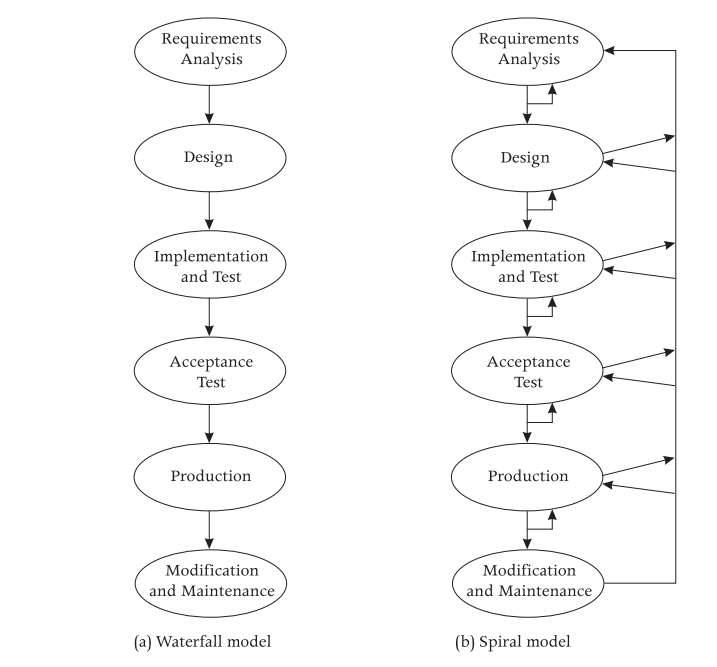
\includegraphics[width=0.8\textwidth]{media/software-life-cycle.png}
    \fonte{\citeonline{barbaraLiskov}}
    \label{fig:ciclo-vida}
\end{figure}

Para este trabalho, os requistos foram definidos no \autoref{cap:metodologia}. Da mesma forma, a fase de manutenção não será abordada, pois o foco é a construção do sistema.

\section{Design}
Esta seção utiliza como entrada os requisitos funcionais e não-funcionais definidos no \autoref{cap:metodologia} para descrever o design do sistema utilizando \acrfull{ams} e \acrfull{ddd}.

Inicialmente, é importante definir os conceitos chaves do sistema, bem como seus relacionamentos. A \autoref{fig:modelo_conceitual} ilustra as abstrações do sistema.

\begin{figure}[H]
    \centering
    \caption{Modelo conceitual do sistema}
    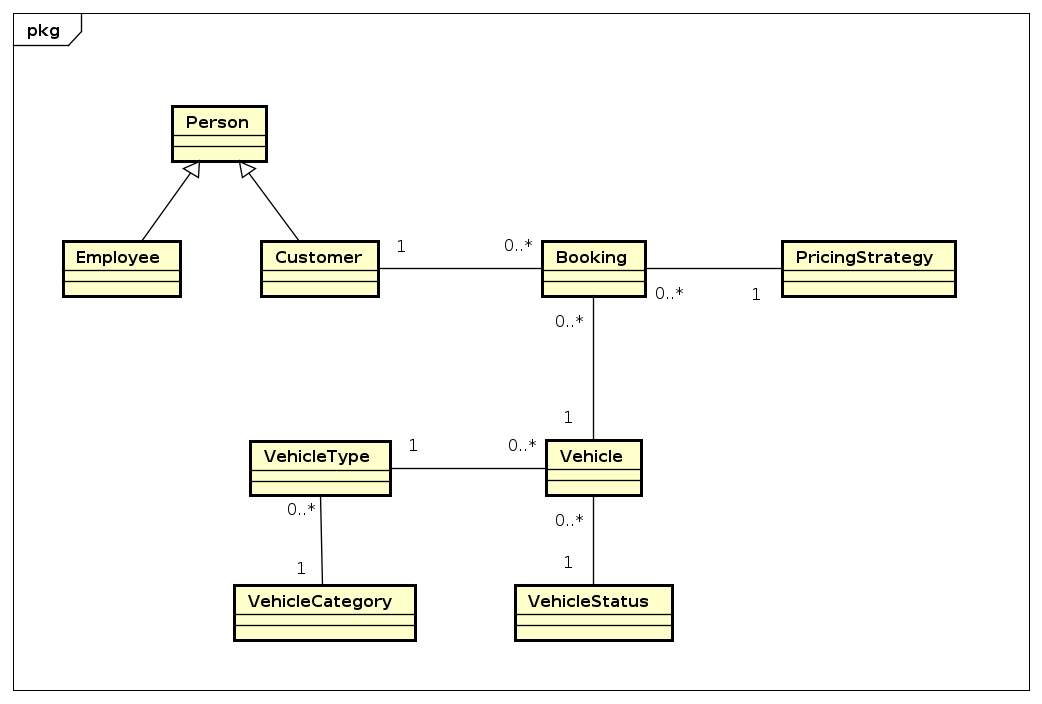
\includegraphics[width=0.8\textwidth]{media/modelo_conceitual.png}
    \fonte{o autor}
    \label{fig:modelo_conceitual}
\end{figure}

O sistema tem como componente principal a entidade \texit{Booking} que está relacionada com um \english{Vehicle} e um \english{Customer}. Cada \english{Vehicle} possui um \english{VehicleType} que tem como função agrupar veículos com características similares. Além disso, cada reserva contém uma \english{PricingStrategy} que é responsável por calcular o preço da reserva baseado em diferentes critérios. Um \english{Customer} é um subtipo de \english{Person}. Da mesma forma, o \english{Employee} é um subtipo de \english{Person}.

No contexto deste caso de uso, as abstrações \english{Booking}, \english{Vehicle}, \english{Customer}, \english{Person} e \english{Employee} possuem identidade e ciclo de vida próprios. Portanto, são entidades. Por outro lado, \english{VehicleType} e \english{PricingStrategy} são \acrfull{vo}, pois não possuem identidade própria e são imutáveis. 

\subsection{Bounded Contexts}
Após ter identificado as entidades e \acrfull{vo}, é necessário definir os \acrfull{bc} do sistema. \citeonline{evans2004ddd} define \acrshort{bc} como um limite lógico dentro do qual um modelo é consistente. Além disso, cada \acrshort{bc} possui um ou mais \english{Aggregates}. Nesse sentido, a \autoref{fig:bounded_contexts} ilustra os \acrshort{bc} do sistema.

\begin{figure}[H]
    \centering
    \caption{Bounded Contexts do sistema}
    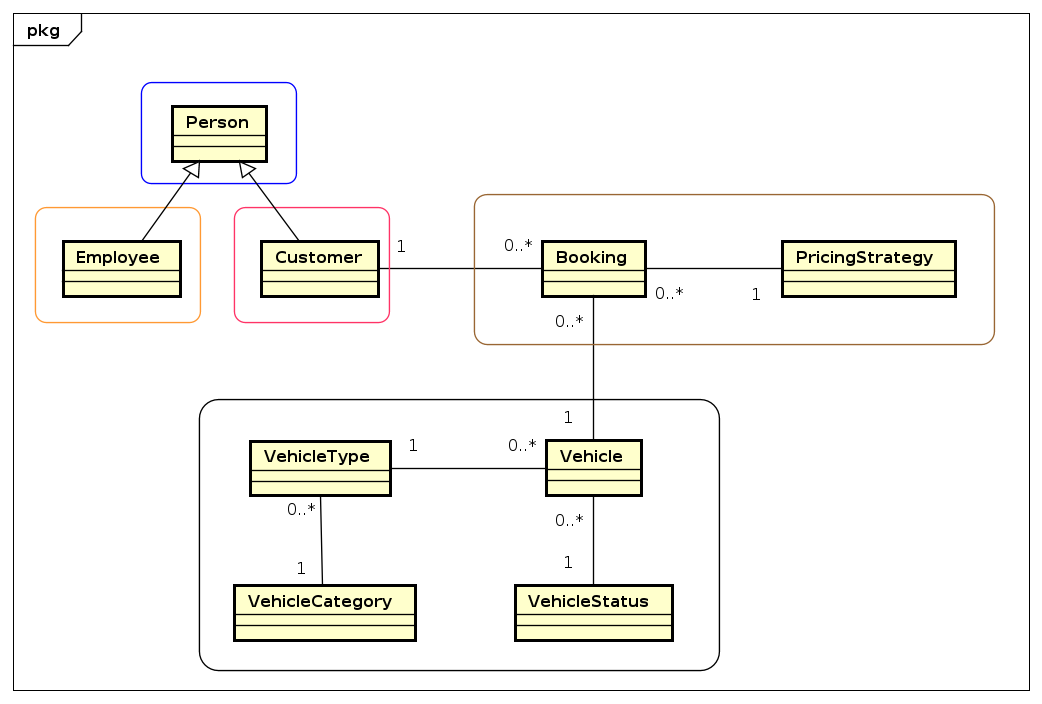
\includegraphics[width=0.8\textwidth]{media/bounded_contexts.png}
    \fonte{o autor}
    \label{fig:bounded_contexts}
\end{figure}

Ao todo, o sistema possui 5 \acrfull{bc}:
\begin{itemize}
    \item \english{Person}: Responsável por gerenciar informações de pessoas e autenticação.
    \item \english{Customer}: Realiza o gerenciamento informações de clientes.
    \item \english{Employee}: Responsável por gerenciar informações de funcionários.
    \item \english{Vehicle}: Está relacionado a estoque de veículos e tipos de veículo.
    \item \english{Booking}: Responsável por gerenciar informações de reservas e estratégias de precificação.
\end{itemize}

\subsection{Microsserviços}
Com os \acrshort{bc} definidos, é possível definir os limites de cada microsserviço. Seguindo as melhores práticas revisadas no \autoref{cap:trabalhos}, cada \acrshort{bc} é mapeado em um microsserviço. A \autoref{fig:microsservicos} ilustra a divisão dos microsserviços.

\begin{figure}[H]
    \centering
    \caption{Microsserviços do sistema}
    \fbox{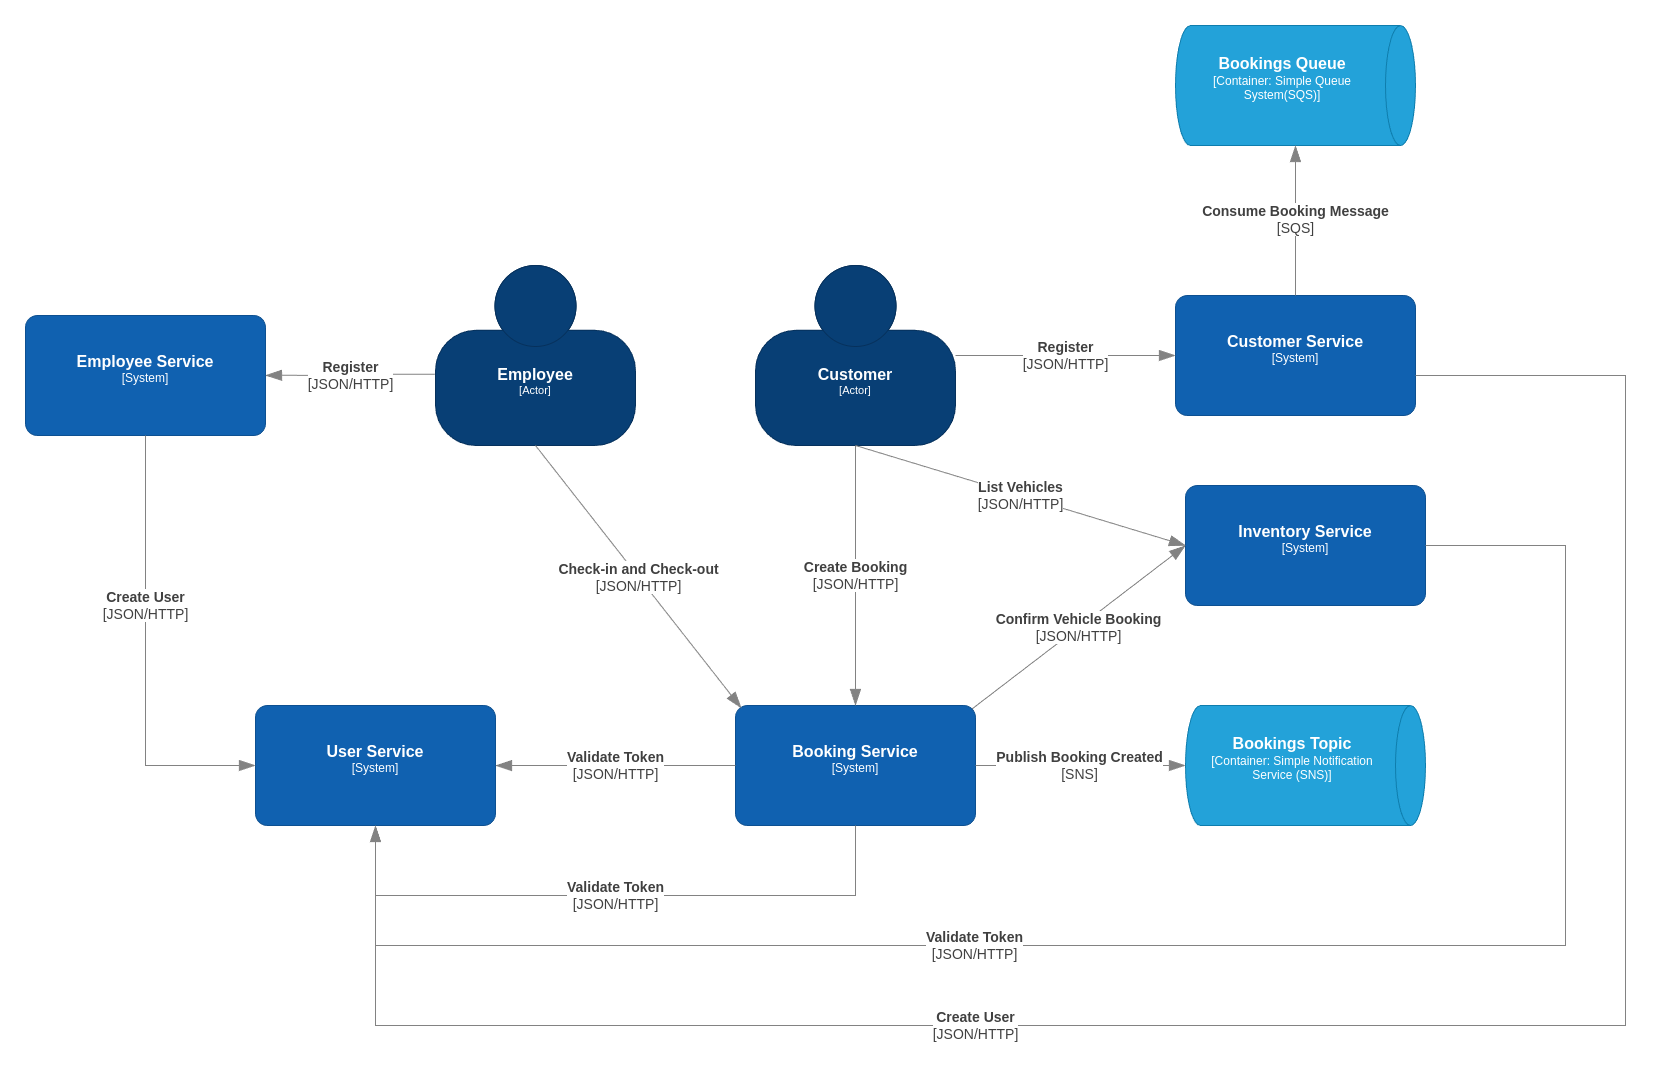
\includegraphics[width=0.8\textwidth]{media/microsservicos.png}}
    \fonte{o autor}
    \label{fig:microsservicos}
\end{figure}

Cada microsserviço é responsável por um \acrshort{bc} e possui sua própria base de dados. O \english{User Service} realiza o cadastro e login de todos usuários do sistema, além de validar \english{tokens} de autenticação. O \english{Customer Service} lida com informações de clientes. Esse serviço também consome uma fila de mensagens de reservas e atualiza um contador de reservas para cada usuário. O \english{Employee Service} gerencia informações de funcionários. O \english{Vehicle Service} trata informações de veículos como quantidade em estoque, marca, modelo, cor e tipo. Por fim, o \english{Booking Service} gerencia informações de reservas e estratégias de precificação.

\subsection{Principais casos de uso}
A seguir são detalhadas as interações entre os microsserviços para os principais casos de uso do sistema. Especificamente, são descritos os casos de uso que compõem o ciclo de vida de uma reserva ilustrado no \autoref{fig:ciclo-reserva}.

\begin{figure}[H]
    \centering
    \caption{Ciclo de vida de uma reserva}
    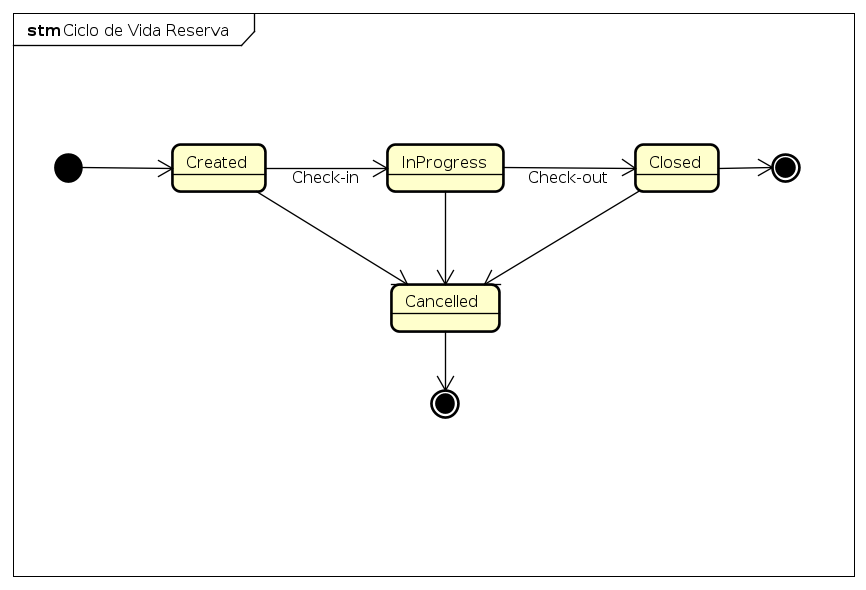
\includegraphics[width=0.8\textwidth]{media/ciclo-reserva.png}
    \fonte{o autor}
    \label{fig:ciclo-reserva}
\end{figure}

\subsubsection{Criar reserva}
A \autoref{fig:realizar-reserva} ilustra o fluxo de criação de uma reserva. Inicialmente, o cliente realiza o login no \english{User Service} e recebe um token como resposta. Em seguida, ele acessa o \english{Vehicle Service} para verificar a disponibilidade de veículos. Esse verifica se o usuário está autenticado realizando uma chamada para o \english{User Service}. Caso o usuário esteja autenticado, o \english{Vehicle Service} retorna a lista de veículos disponíveis. Posteriormente, O cliente seleciona um veículo e realiza a reserva no \english{Booking Service}. Esse serviço envia uma requisição para o \english{Inventory Service} para decrementar a quantidade de veículos disponíveis e confirmar a reserva. Por fim, o \english{Booking Service} retorna a confirmação da reserva.

\begin{figure}[H]
    \centering
    \caption{Criar reserva}
    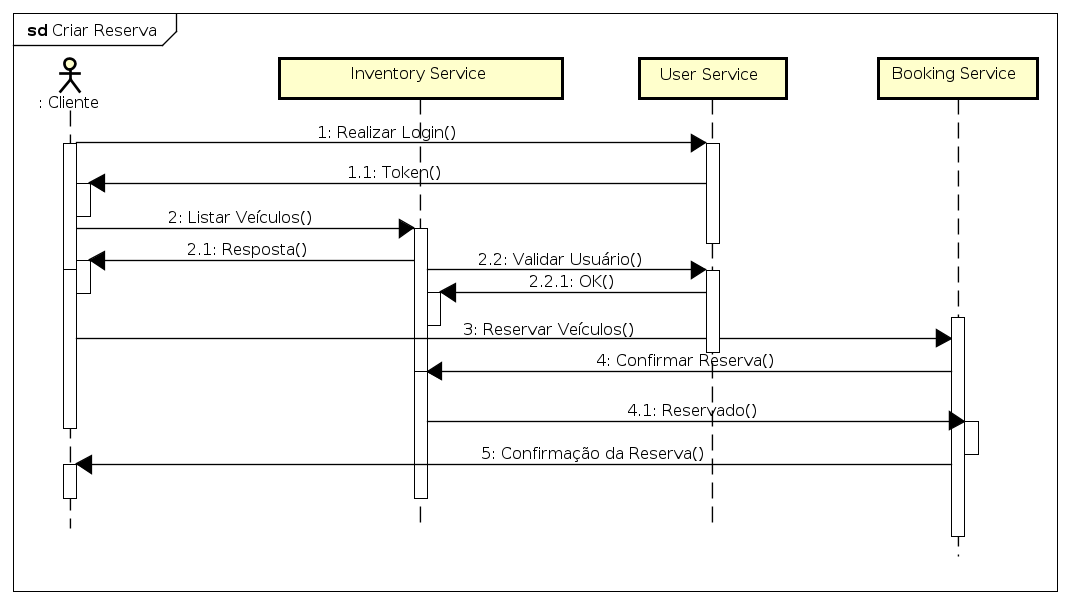
\includegraphics[width=0.8\textwidth]{media/criar-reserva.png}
    \fonte{o autor}
    \label{fig:realizar-reserva}
\end{figure}

\subsubsection{Realizar check-in}
A \autoref{fig:realizar-checkin} ilustra o fluxo de realizar um check-in. Primeiramente, o funcionário realiza o login no \english{User Service} e recebe um token como resposta. Em seguida, ele acessa o \english{Booking Service} para realizar o check-in. Esse serviço verifica se o usuário está autenticado realizando uma chamada para o \english{User Service}. Caso o usuário esteja autenticado, o \english{Booking Service} realiza o check-in e retorna a confirmação.

\begin{figure}[H]
    \centering
    \caption{Realizar check-in}
    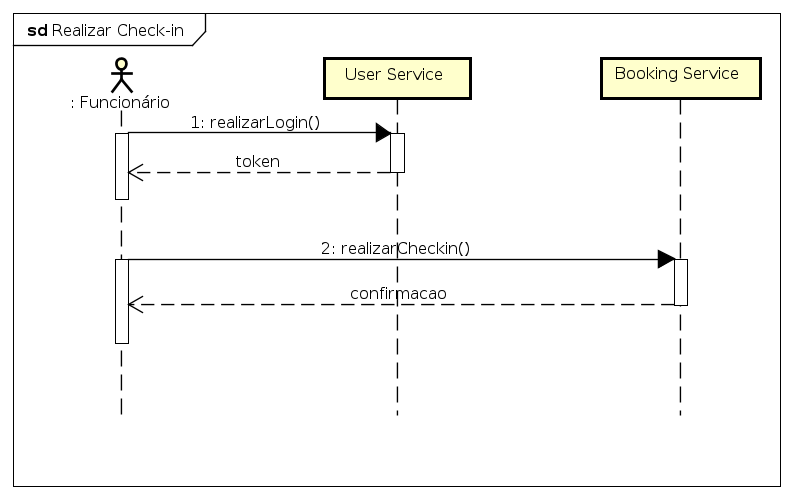
\includegraphics[width=0.8\textwidth]{media/realizar-checkin.png}
    \fonte{o autor}
    \label{fig:realizar-checkin}
\end{figure}

\subsubsection{Realizar check-out}
A \autoref{fig:realizar-checkout} ilustra o fluxo de realizar um check-out. Inicialmente, o funcionário realiza a autenticação no \english{User Service} e recebe um token como resposta. Posteriormente, ele acessa o \english{Booking Service} para realizar o check-out. Esse serviço verifica se o usuário está autenticado realizando uma chamada para o \english{User Service}. Caso o usuário esteja autenticado, o \english{Booking Service} realiza o check-out e retorna a confirmação.

\begin{figure}[H]
    \centering
    \caption{Realizar check-out}
    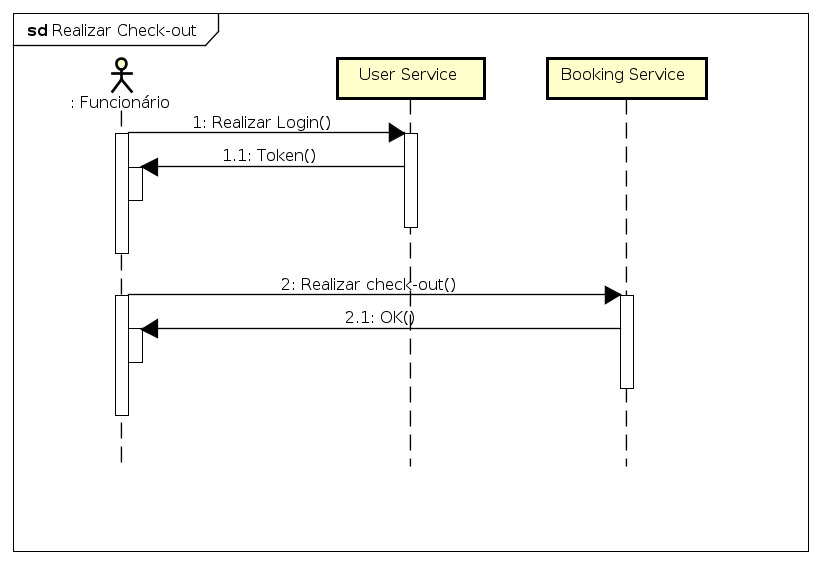
\includegraphics[width=0.8\textwidth]{media/realizar-checkout.png}
    \fonte{o autor}
    \label{fig:realizar-checkout}
\end{figure}

\subsection{User Service}
A \autoref{fig:user-service} apresenta os principais componentes do \english{User Service} na Arquitetura Hexagonal.

\begin{figure}[H]
    \centering
    \caption{User Service}
    \fbox{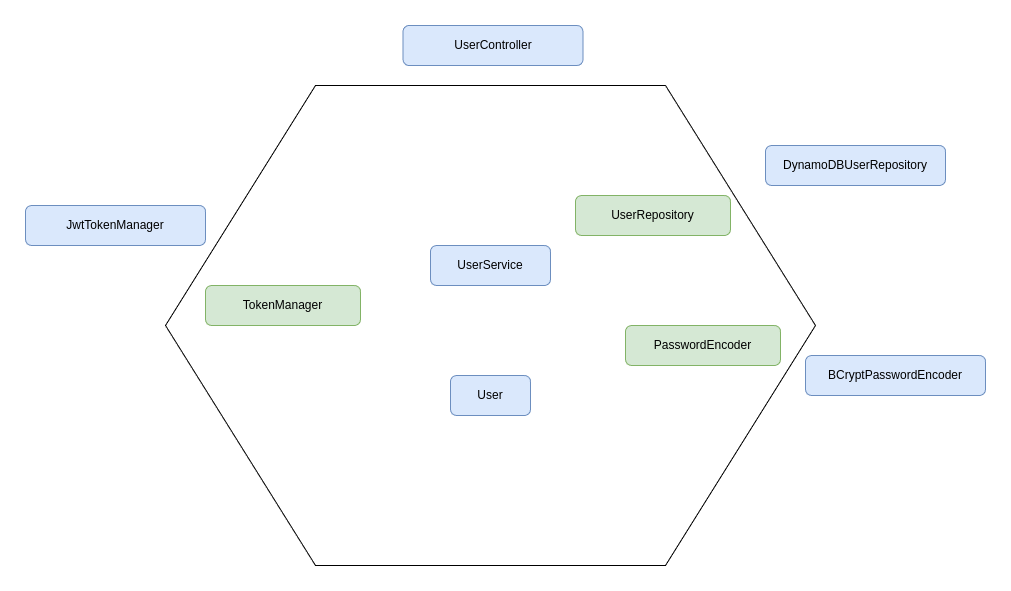
\includegraphics[width=0.8\textwidth]{media/user-service.png}}
    \fonte{o autor}
    \label{fig:user-service}
\end{figure}

Os componentes do \english{Application core} são: \english{User} e \english{UserService}. A aplicação possui as seguintes portas: \english{UserRepository}, \english{PasswordEncoder} e \english{TokenManager}. Por fim, os adaptadores \english{UserController}, \english{DynamoDBUserRepository}, \english{BCryptPasswordEncoder} e \english{JwtTokenManager} são responsáveis por integrar a aplicação com o mundo externo.

\subsection{Customer Service}
A \autoref{fig:customer-service} apresenta os principais componentes do \english{Customer Service} na Arquitetura Hexagonal.

\begin{figure}[H]
    \centering
    \caption{Customer Service}
    \fbox{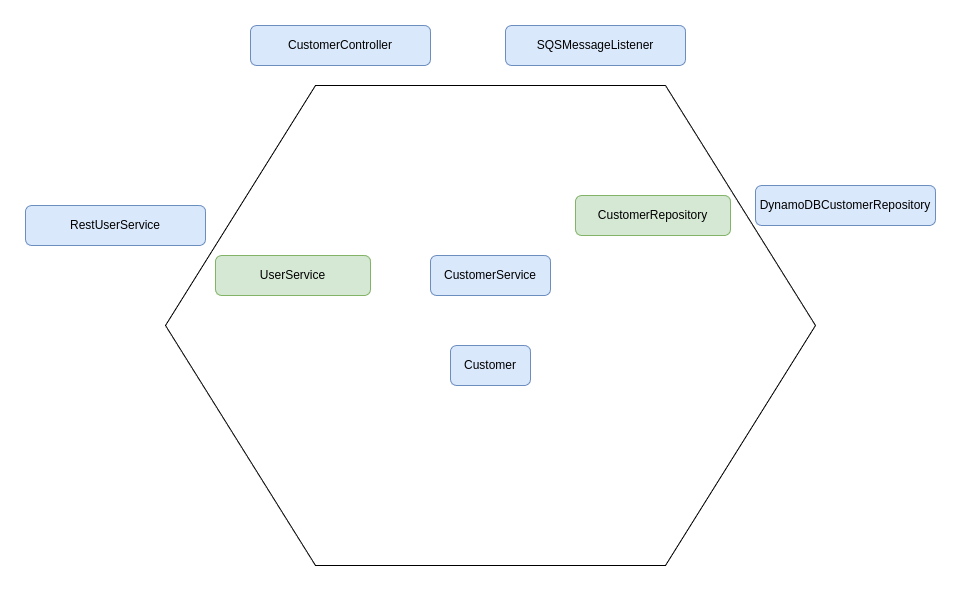
\includegraphics[width=0.8\textwidth]{media/customer-service.png}}
    \fonte{o autor}
    \label{fig:customer-service}
\end{figure}

Nesse serviço, o \english{Application core} é composto por  \english{Customer} e \english{CustomerService}. As portas são: \english{CustomerRepository} e \english{UserService}. Por fim, os adaptadores são: \english{CustomerController}, \english{RestUserService} \english{DynamoDBCustomerRepository} e \english{SQSMessageListener}.

\subsection{Employee Service}
A \autoref{fig:employee-service} apresenta os principais componentes do \english{Employee Service} na Arquitetura Hexagonal.

\begin{figure}[H]
    \centering
    \caption{Employee Service}
    \fbox{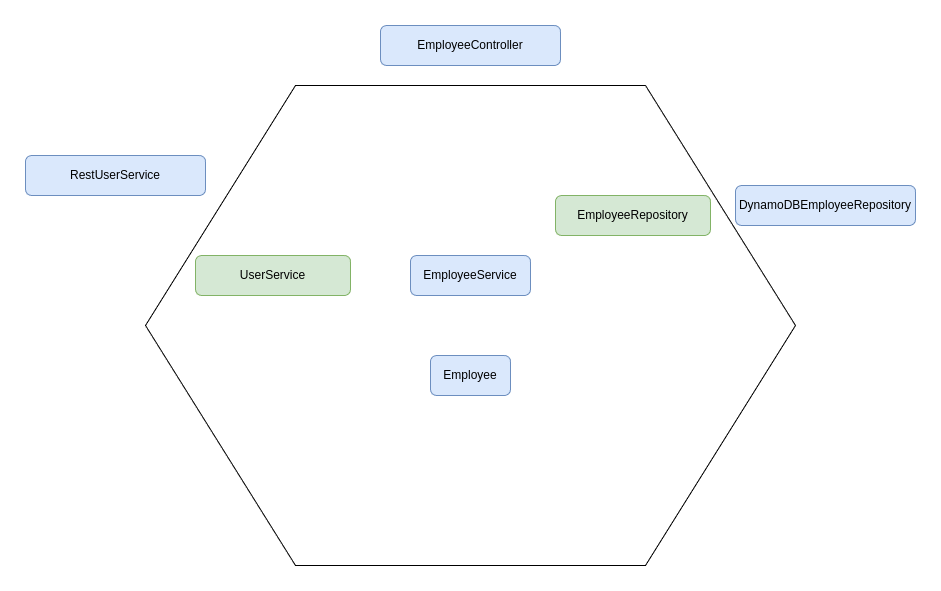
\includegraphics[width=0.8\textwidth]{media/employee-service.png}}
    \fonte{o autor}
    \label{fig:employee-service}
\end{figure}

O \english{Application core} é composto por \english{Employee} e \english{EmployeeService}. As portas são: \english{EmployeeRepository} e \english{UserService}. Por fim, os adaptadores são: \english{EmployeeController}, \english{DynamoDBEmployeeRepository} e \english{RestUserService}.

\subsection{Inventory Service}
Essa seção apresenta os principais componentes do \english{Inventory Service} na Arquitetura Hexagonal, ilustrados na \autoref{fig:inventory-service}.

\begin{figure}[H]
    \centering
    \caption{Inventory Service}
    \fbox{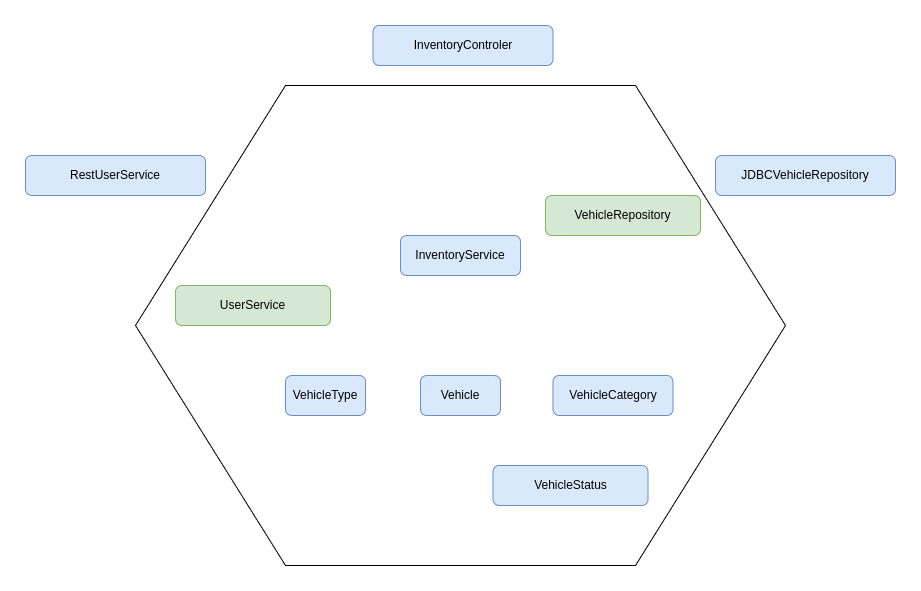
\includegraphics[width=0.8\textwidth]{media/inventory-service.png}}
    \fonte{o autor}
    \label{fig:inventory-service}
\end{figure}

Nessa aplicação, o \english{Application core} é composto por \english{Vehicle}, \english{VehicleType}, \english{VehicleCategory}, \english{VehicleStatus} e \english{InventoryService}. As portas são: \english{VehicleRepository} e \english{UserService}. Por fim, os adaptadores são: \english{InventoryController}, \english{JDBCInventoryRepository} e \english{RestUserService}.

\subsection{Booking Service}
A \autoref{fig:booking-service} apresenta os principais componentes do \english{Booking Service} na Arquitetura Hexagonal.

\begin{figure}[H]
    \centering
    \caption{Booking Service}
    \fbox{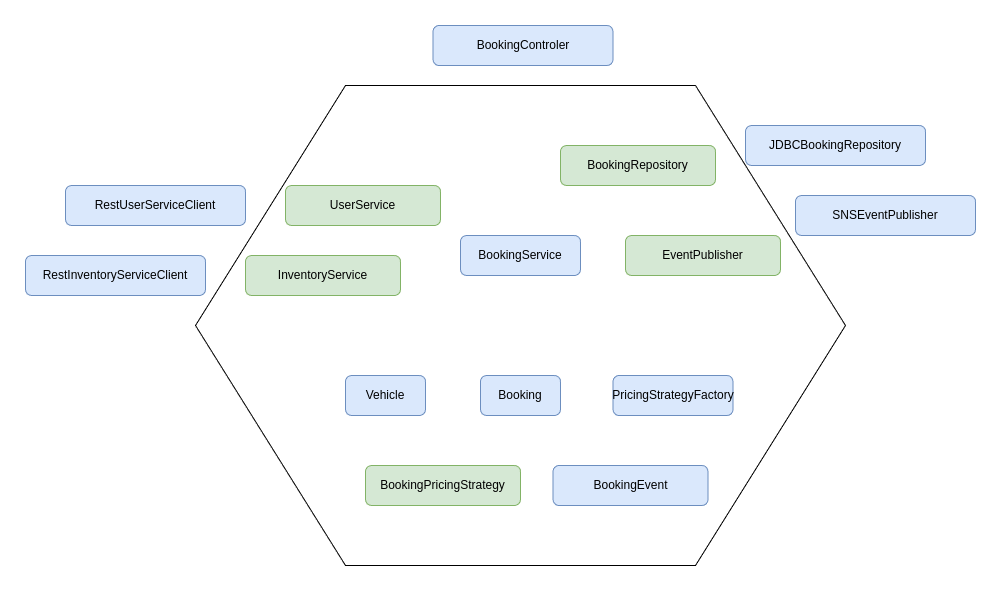
\includegraphics[width=0.8\textwidth]{media/booking-service.png}}
    \fonte{o autor}
    \label{fig:booking-service}
\end{figure}

O \english{Application core} é composto por \english{Booking}, \english{BookingPricingStrategy}, \english{Vehicle}, \english{PricingStrategyFactory}, \english{BookingEvent} e \english{BookingService}. As portas são: \english{BookingRepository}, \english{EventPublisher}, \english{UserService} e \english{InventoryService}. Por fim, os adaptadores são: \english{BookingController}, \english{JDBCBookingRepository}, \english{SNSEventPublisher}, \english{RestUserServiceClient} e \english{RestInventoryServiceClient}.

\section{Implementação}
Esta seção apresenta os trechos de código chaves para a implementação do caso de uso. O código completo pode ser encontrado no repositório do projeto \footnote{\url{https://github.com/C0lliNN/CarroFacil}}.

\subsection{Login de usuário}
O \autoref{cod:login} apresenta o método para realizar login de um usuário. Esse método recebe um \english{LoginRequest} contendo o email e senha do usuário. Em seguida, ele busca o usuário no repositório e compara a senha informada com a senha armazenada no banco de dados. Caso a senha seja válida, o método retorna um \english{UserResponse} contendo o token de autenticação. O procedimento lança exceções caso o email não seja encontrado ou a senha seja inválida.

\begin{codigo}[H]
    \begin{lstlisting}[language=Java]
    public class UserService {
        private final UserRepository repository;
        private final PasswordEncoder passwordEncoder;
        private final TokenManager tokenManager;

        public UserResponse login(LoginRequest request) {
            User user = repository.findByEmail(request.email()).
                    orElseThrow(() -> new EmailNotFoundException("The email '%s' could not be found.", request.email()));

            if (!passwordEncoder.comparePasswordAndHash(request.password(), user.getPassword())) {
                throw new IncorrectPasswordException("The provided password is incorrect.");
            }

            return createUserResponseWithToken(user);
        }

        // Other methods
    }
    \end{lstlisting}
    \caption{Método para realizar login}
    \label{cod:login}
\end{codigo}

\subsection{Cadastro de Cliente}
O \autoref{cod:cadastro-cliente} apresenta o método para realizar o cadastro de um cliente. Esse método recebe um \english{RegisterRequest} contendo o nome, email e senha do cliente. Em seguida, ele realiza o cadastro do usuário no \english{User Service} e cria um cliente no \english{Customer Service}. Por fim, o método retorna um \english{CustomerResponse} contendo as informações do cliente.

\begin{codigo}[H]
    \begin{lstlisting}[language=Java]
        public class CustomerService {
            private final UserServiceClient userServiceClient;
            private final CustomerRepository customerRepository;
        
            public CustomerResponse register(RegisterRequest request) {
                User user = userServiceClient.register(request.name(), request.email(), request.password());
        
                Customer customer = Customer.builder()
                        .name(request.name())
                        .userId(user.getId())
                        .build();
        
                return CustomerResponse.fromCustomer(customerRepository.save(customer), user);
            }

        // Other methods
    }
    \end{lstlisting}
    \caption{Método para realizar cadastro de cliente}
    \label{cod:cadastro-cliente}
\end{codigo}

\subsection{Realizar Reserva}
O \autoref{cod:realizar-reserva} apresenta o método para realizar uma reserva. Esse método recebe um \english{BookingRequest} contendo as informações da reserva. Em seguida, ele busca o veículo no \english{Inventory Service} e realiza a reserva no \english{Booking Service}. Além disso, o método publica um evento que poderá ser consumido por outros serviços. Por fim, o método retorna um \english{BookingResponse} contendo as informações da reserva.

\begin{codigo}[H]
    \begin{lstlisting}[language=Java]
        public class BookingService {
            private BookingRepository bookingRepository;
            private InventoryClient inventoryClient;
            private BookingEventPublisher bookingEventPublisher;

            public BookingResponse createBooking(BookingRequest bookingRequest) {
                Booking booking = bookingRequest.createBooking();
                Vehicle vehicle = inventoryClient.getVehicle(booking.getVehicleId());
                booking.setVehicle(vehicle);
        
                booking = bookingRepository.save(booking);
        
                bookingEventPublisher.publishBookingEvent(
                        new BookingEvent(booking.getId(), booking.getUserId(), vehicle.getId())
                );
        
                return BookingResponse.from(booking);
            }

            // Other methods
        }
    \end{lstlisting}
    \caption{Método para criar reserva}
    \label{cod:realizar-reserva}
\end{codigo}

\subsection{Realizar Check-in}
O \autoref{cod:realizar-check-in} contém o código necessário para realizar um check-in. No \english{BookingService} é possível ver o método \english{checkin} que recebe o id da reserva e realiza o check-in. Esse método busca a reserva no repositório, realiza o check-in e salva a reserva. Toda a operação é executada em uma transação ACID com nível de isolamento de serialização para previnir checkins duplicados. O método \english{checkIn} da classe \english{Booking} é responsável por validar o estado da reserva, atualizar o status e a data de check-in.

\begin{codigo}[H]
    \begin{lstlisting}[language=Java]
        public class BookingService {
            private BookingRepository bookingRepository;
            private InventoryClient inventoryClient;
            private BookingEventPublisher bookingEventPublisher;

            @Transactional(isolation = Isolation.SERIALIZABLE)
            public void checkin(int bookingId) {
                Booking booking = bookingRepository.findById(bookingId)
                        .orElseThrow(() -> new EntityNotFoundException("Booking not found"));
        
                booking.checkIn();
                bookingRepository.save(booking);
            }

            // Other methods
        }

        public class Booking {
            // other fields and methods

            public void checkIn() {
                if (status != Status.CREATED) {
                    throw new InvalidBookingStateException("Booking is not in CREATED state");
                }
        
                status = Status.IN_PROGRESS;
                checkedInAt = LocalDateTime.now();
            }
        }
    \end{lstlisting}
    \caption{Métodos para realizar check-in}
    \label{cod:realizar-check-in}
\end{codigo}

\subsection{Realizar Check-out}
O \autoref{cod:realizar-check-out} contém o código necessário para realizar um check-out. No \english{BookingService} é possível ver o método \english{checkout} que recebe o id da reserva e realiza o check-out. Esse método busca a reserva no repositório, realiza o check-out e salva a reserva. Toda a operação é executada em uma transação ACID com nível de isolamento de serialização para previnir checkouts duplicados. O método \english{checkOut} da classe \english{Booking} é responsável por validar o estado da reserva, atualizar o status e a data de check-out.

\begin{codigo}[H]
    \begin{lstlisting}[language=Java]
        public class BookingService {
            private BookingRepository bookingRepository;
            private InventoryClient inventoryClient;
            private BookingEventPublisher bookingEventPublisher;

            @Transactional(isolation = Isolation.SERIALIZABLE)
            public void checkout(int bookingId) {
                Booking booking = bookingRepository.findById(bookingId)
                        .orElseThrow(() -> new EntityNotFoundException("Booking not found"));

                booking.checkOut();
                bookingRepository.save(booking);
            }

            // Other methods
        }

        public class Booking {
            // other fields and methods

            public void checkOut() {
                if (status != Status.IN_PROGRESS) {
                    throw new InvalidBookingStateException("Booking is not in IN_PROGRESS state");
                }

                status = Status.CLOSED;
                checkedOutAt = LocalDateTime.now();
            }
        }
    \end{lstlisting}
    \caption{Métodos para realizar check-out}
    \label{cod:realizar-check-out}
\end{codigo}

\subsection{Comunicação síncrona entre Microsserviços}
O \autoref{cod:rest-inventory-client} demonstra como a comunicação síncrona entre microsserviços é realizada. O método \english{getVehicle} da classe \english{RestInventoryClient} é responsável por obter um veículo do \english{Inventory Service}. Esse método utiliza o \english{RestTemplate} para realizar uma requisição \acrshort{http} para \english{Inventory Service}. É importante notar que a classe \english{RestInventoryClient} implementa a interface de domínio \english{InventoryClient}. Dessa forma o dominio não está acoplado ao mecanismo de comunicação.

\begin{codigo}[H]
    \begin{lstlisting}[language=Java]
        public class RestInventoryClient implements InventoryClient {
            private RestTemplate restTemplate;
            private String baseUrl;

            @Override
            public Vehicle getVehicle(int id) {
                HttpHeaders headers = new HttpHeaders();
                headers.set("Authorization", "Bearer " + getToken());
                HttpEntity<VehicleResponse> entity = new HttpEntity<>(headers);

                ResponseEntity<VehicleResponse> response = restTemplate.exchange(baseUrl + "/vehicles/{id}", HttpMethod.GET, entity, VehicleResponse.class, id);
                if (response.getStatusCode().value() == 404) {
                    throw new EntityNotFoundException("Vehicle not found");
                }

                if (response.getStatusCode().isError()) {
                    throw new RuntimeException("Error while fetching vehicle");
                }

                return response.getBody().toVehicle();
            }
        }
    \end{lstlisting}
    \caption{Método para obter um veículo do \english{Inventory Service}}
    \label{cod:rest-inventory-client}
\end{codigo}

\subsection{Comunicação assíncrona entre Microsserviços}
O \autoref{cod:comunicacao-assincrona} apresenta como a comunicação assíncrona entre microsserviços é realizada. A classe \english{SNSEventPublisher} é responsável por publicar eventos de reserva no \english{Booking Service}. O método \english{publishBookingEvent} recebe um evento de reserva, serializa o evento e publica no tópico \acrshort{sns}. Por outro lado, a classe \english{SQSListener} é responsável por ouvir eventos de reserva no \english{Customer Service}. O método \english{listen} recebe uma mensagem do \acrshort{sqs}, desserializa a mensagem e incrementa o contador de reservas do usuário. Da mesma forma que na comunicação síncrona, o domínio não está acoplado ao mecanismo de comunicação.

\begin{codigo}[H]
    \begin{lstlisting}[language=Java]
        // class in Booking Service
        public class SNSEventPublisher implements BookingEventPublisher {
            private final SnsClient snsClient;
            private final ObjectMapper objectMapper;

            private String topicArn;

            public void publishBookingEvent(BookingEvent bookingEvent) {
                String message = objectMapper.writeValueAsString(bookingEvent);

                PublishRequest request = PublishRequest.builder()
                        .topicArn(topicArn)
                        .message(message)
                        .build();

                PublishResponse response = snsClient.publish(request);
            }
        }

        // class in Customer service
        public class SQSListener {
            private final CustomerService service;
            private final ObjectMapper objectMapper;

            @SqsListener(queueNames = "${aws.queues.bookings}")
            public void listen(Message message) {
                try {
                    MessageBody body = objectMapper.readValue(message.body(), MessageBody.class);
                    BookingMessage bookingMessage = objectMapper.readValue(body.getMessage(), BookingMessage.class);

                    log.info("Received message: {}", bookingMessage);

                    service.incrementBookingsCount(bookingMessage.getUserId());
                } catch (Exception e) {
                    throw new RuntimeException("Error while processing message", e);
                }
            }
        }

    \end{lstlisting}
    \caption{Código para realizar comunicação assíncrona entre microsserviços}
    \label{cod:comunicacao-assincrona}
\end{codigo}

\section{Testes}
Esta seção apresenta os testes realizados para validar os requisitos funcionais e não funcionais do sistema.

\subsection{Testes Unitários}
Os testes unitários foram realizados utilizando o \english{framework} JUnit. O \autoref{cod:unitario-simples} apresenta um teste unitário simples para o método \english{checkIn} da classe \english{Booking}. Esse teste verifica se o status da reserva é alterado para \english{IN\_PROGRESS} e se a data de check-in é definida quando o status é \english{CREATED}. Além disso, o teste verifica se uma exceção é lançada quando o status não é \english{CREATED}.

\begin{codigo}[H]
    \begin{lstlisting}[language=Java]
        @Nested
        @DisplayName("checkIn method")
        class CheckInMethod {

            @Test
            @DisplayName("should change status to IN_PROGRESS and set checkedInAt to current time when status is CREATED")
            void shouldChangeStatusToInProgressAndSetCheckedInAtToCurrentTimeWhenStatusIsCreated() {
                Booking booking = new Booking();
                booking.setStatus(Booking.Status.CREATED);

                booking.checkIn();

                assertEquals(Booking.Status.IN_PROGRESS, booking.getStatus());
                assertNotNull(booking.getCheckedInAt());
            }

            @Test
            @DisplayName("should throw InvalidBookingStateException when status is not CREATED")
            void shouldThrowInvalidBookingStateExceptionWhenStatusIsNotCreated() {
                Booking booking = new Booking();
                booking.setStatus(Booking.Status.CANCELLED);

                assertThrows(InvalidBookingStateException.class, booking::checkIn);
            }
        }
    \end{lstlisting}
    \caption{Teste unitário simples}
    \label{cod:unitario-simples}
\end{codigo}

\subsection{Testes de Integração}
O framework Mockito é utilizado para execucação dos testes de integração de maneira isolada. O \autoref{cod:test-integracao} apresenta um teste de integração para o método \english{checkin} da classe \english{BookingService}. Esse teste verifica se uma exceção é lançada quando a reserva não é encontrada e se o status da reserva é alterado para \english{IN\_PROGRESS} quando a reserva é encontrada. Além disso, o teste verifica se o método \english{save} do repositório é chamado uma vez.

\begin{codigo}[H]
    \begin{lstlisting}[language=Java]
        @Nested
        @DisplayName("method: checkin")
        class Checkin {

            @Mock
            private BookingRepository bookingRepository;

            @Test
            @DisplayName("when booking is not found, then it should throw a EntityNotFoundException")
            void whenBookingIsNotFound_thenItShouldThrowAEntityNotFoundException() {
                assertThrows(EntityNotFoundException.class, () -> bookingService.checkin(1));
            }

            @Test
            @DisplayName("when all operations are successful, then it should checkin the booking")
            void whenAllOperationsAreSuccessful_thenItShouldCheckinTheBooking() {
                when(bookingRepository.findById(1)).thenReturn(Optional.of(booking));
                when(bookingRepository.save(booking)).thenReturn(booking);

                bookingService.checkin(1);

                assertEquals(Booking.Status.IN_PROGRESS, booking.getStatus());
                verify(bookingRepository, times(1)).save(booking);
            }
        }
    \end{lstlisting}
    \caption{Teste de integração}
    \label{cod:test-integracao}
\end{codigo}

\subsection{Testes de Sistema}
Os testes de sistema são realizados com auxílio do Testcontainers, uma ferramenta que permite a execucação de testes de sistema com alto nível de confibilidade através da criação de containers Docker. O \autoref{cod:test-sistema} apresenta um teste de sistema para a rota \english{POST /bookings}. Esse teste verifica se uma requisição inválida retorna um código de status 400 e se uma requisição válida retorna um código de status 201.

\begin{codigo}[H]
    \begin{lstlisting}[language=Java]
        @Nested
        @DisplayName("POST /bookings")
        class PostBookings {

            @Test
            @DisplayName("When request is not valid, then it should return 400 Bad Request")
            void whenRequestIsNotValid_shouldReturn400() throws Exception {
                mockMvc.perform(post("/bookings")
                                .contentType(MediaType.APPLICATION_JSON)
                                .content("{" +
                                        "\"vehicleId\": 1," +
                                        "\"userId\": \"\"," +
                                        "\"startTime\": \"2023-01-01T00:00:00\"," +
                                        "\"endTime\": \"2023-01-02T00:00:00\"" +
                                        "}"))
                        .andExpect(status().isBadRequest());
            }

            @Test
            @WithMockEmployee
            @DisplayName("when request is valid, then it should return 201 Created")
            void whenRequestIsValid_shouldReturn201() throws Exception {
                when(inventoryClient.getVehicle(1)).thenReturn(new Vehicle(1, "vehicle", "model", 2023));

                mockMvc.perform(post("/bookings")
                                .contentType(MediaType.APPLICATION_JSON)
                                .content("{" +
                                        "\"vehicleId\": 1," +
                                        "\"userId\": \"user-id\"," +
                                        "\"startTime\": \"2026-01-01T00:00:00\"," +
                                        "\"endTime\": \"2026-01-02T00:00:00\"" +
                                        "}"))
                        .andExpect(status().isCreated());
            }
        }
    \end{lstlisting}
    \caption{Teste de sistema}
    \label{cod:test-sistema}
\end{codigo}

\subsection{Testes de Carga}
Para os testes de carga, o framework \english{Gatling} é utilizado. O \autoref{cod:test-carga} apresenta um teste de carga para o cenário de reserva. Esse teste simula o cadastro de 100 usuários, a criação de um veículo, a reserva do veículo e o check-in e check-out da reserva. O teste é realizado com 100 usuários simultâneos durante 30 minutos como especificado no \autoref{cap:metodologia}.

\begin{codigo}[H]
    \begin{lstlisting}[language=Java]
        private final int NUM_USERS = 100;
        private final int RAMP_UP_TIME = 30;

        ScenarioBuilder registerScenario = scenario("register")
                .feed(feeder)
                .exec(
                        http("Register Customer")
                                .post(CUSTOMER_BASE_URL + "/register")
                                .header("Content-Type", "application/json")
                                .body(StringBody("{\"name\": \"#{name}\", \"email\": \"#{email}\", \"password\": \"#{password}\"}"))
                                .check(status().is(200))
                                .check(jsonPath("$.token").saveAs("token")))
                .exec(http("Create Vehicle")
                        .put(INVENTORY_BASE_URL + "/vehicles")
                        .header("Content-Type", "application/json")
                        .header("Authorization", "Bearer " + EMPLOYEE_TOKEN)
                        .body(StringBody("{\"typeId\":1,\"make\":\"Hyundai\",\"model\":\"Creta\",\"year\":2024,\"mileage\":10000,\"licensePlate\":\"23525\",\"chassisNumber\":\"252355125\",\"engineNumber\":\"234242\",\"color\":\"white\"}"))
                        .check(status().is(200))
                        .check(jsonPath("$.id").saveAs("vehicleId")))
                .exec(http("Book Vehicle")
                        .post(BOOKING_BASE_URL + "/bookings")
                        .header("Content-Type", "application/json")
                        .header("Authorization", "Bearer #{token}")
                        .body(StringBody("{\"vehicleId\":#{vehicleId},\"startTime\":\"2024-12-03T10:15:30\",\"endTime\":\"2024-12-04T10:15:30\"}"))
                        .check(status().is(201))
                        .check(jsonPath("$.id").saveAs("bookingId")))
                .exec(http("Check in Booking")
                        .patch(BOOKING_BASE_URL + "/bookings/#{bookingId}/check-in")
                        .header("Content-Type", "application/json")
                        .header("Authorization", "Bearer " + EMPLOYEE_TOKEN)
                        .check(status().is(200)))
                .exec(http("Check out Booking")
                        .patch(BOOKING_BASE_URL + "/bookings/#{bookingId}/check-out")
                        .header("Content-Type", "application/json")
                        .header("Authorization", "Bearer " + EMPLOYEE_TOKEN)
                        .check(status().is(200)));


        HttpProtocolBuilder httpProtocol =
                http.enableHttp2();

        {
            setUp(
                    registerScenario.injectClosed(
                            rampConcurrentUsers(0).to(NUM_USERS).during(Duration.ofMinutes(RAMP_UP_TIME))
                    )
            ).protocols(httpProtocol);
        }
    \end{lstlisting}
    \caption{Teste de carga}
    \label{cod:test-carga}
\end{codigo}

\chapter{Resultados e Discussões}
\label{cap:resultados}
Este capítulo apresenta os resultados obtidos com a execução dos testes de carga descritos no \autoref{cap:estudo_caso1}. Além disso, há uma discussão geral sobre o processo de desenvolvimento do caso de uso com a utilização da \acrfull{ams} e \acrfull{ddd}.

\section{Resultados}
Essa seção apresenta uma análise gráfica dos resultados obtidos com a execução dos testes de carga. Os gráficos foram gerados pelo \english{AWS CloudWatch} a partir das métricas coletadas dos serviços de computação e banco de dados da \english{Amazon Web Services} durante a execução dos testes. Os dados apresentados apresentam a média dos serviços.

\subsection{Utilização da CPU}
Na \autoref{fig:cpu-utilization} é possível observar a utilização da CPU durante a execução dos testes de carga. Durante toda a simulação, a utilização de CPU se manteve em torno de 35\%, um valor considerado baixo. Isso indica que o sistema é capaz de suportar um número maior de requisições sem que haja um aumento significativo na utilização de CPU. Esse valor também está abaixo do alvo de 70\% estabelecido anteriormente. 

\begin{figure}[H]
    \centering
    \caption{Utilização da CPU}
    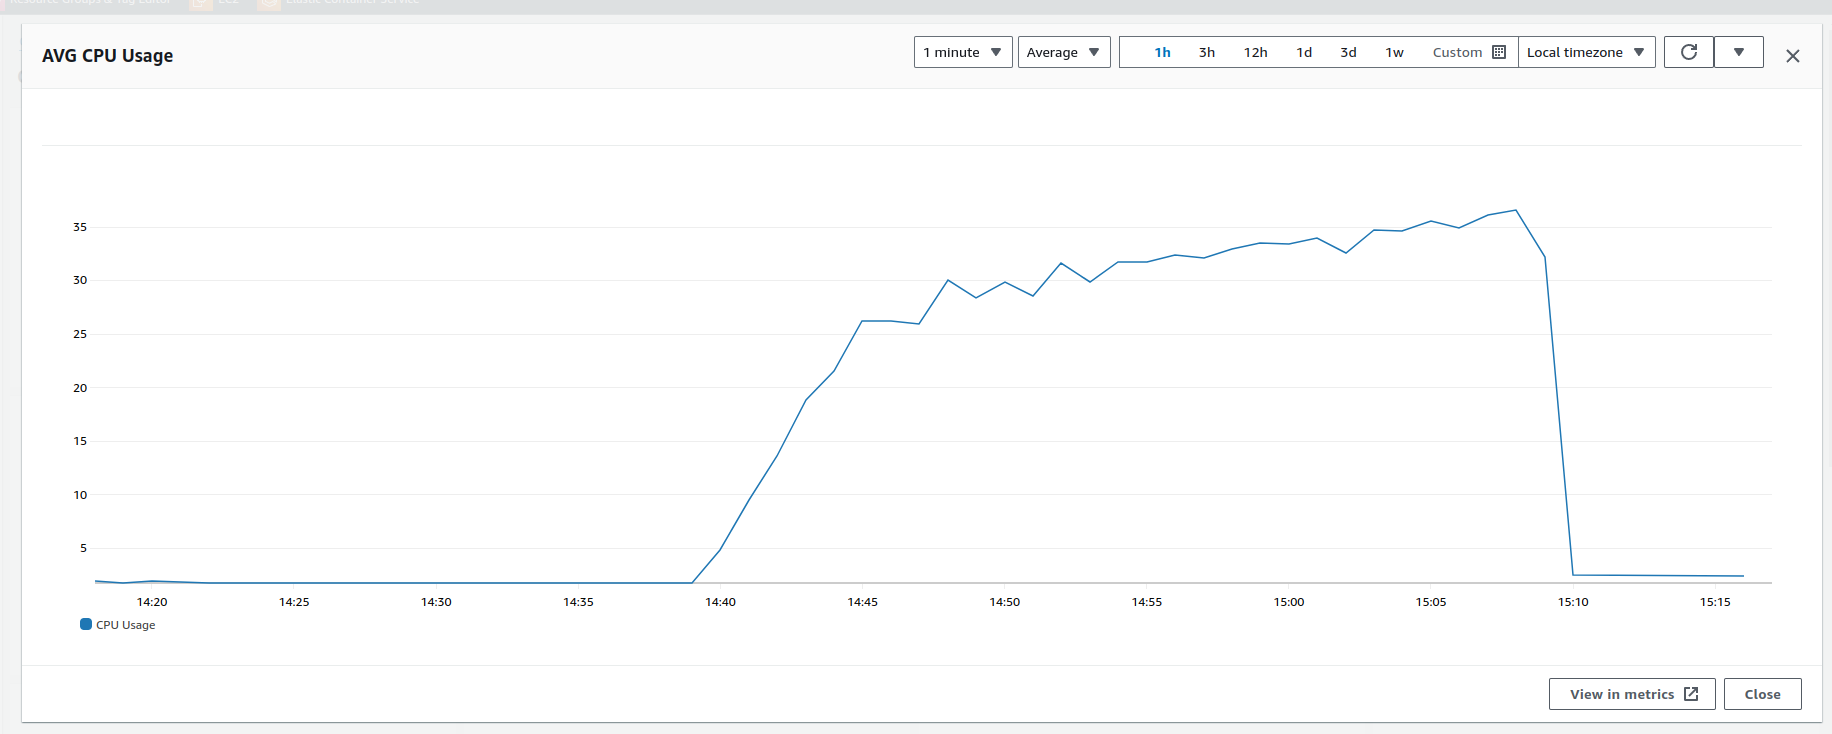
\includegraphics[width=0.8\textwidth]{media/cpu-usage.png}
    \fonte{o autor}
    \label{fig:cpu-utilization}
\end{figure}

\subsection{Utilização da Memória RAM}
Na \autoref{fig:memory-utilization} é possível observar a utilização da memória RAM durante a execução dos testes de carga. Houve um uso muito baixo de memória, com uma média em torno de 7\%. Isso indica que o sistema como um todo é \english{CPU-bound}, termo utilizado para descrever sistemas que são limitados pela CPU e não pela memória. Essa métrica também ficou abaixo do alvo.

\begin{figure}[H]
    \centering
    \caption{Utilização da Memória RAM}
    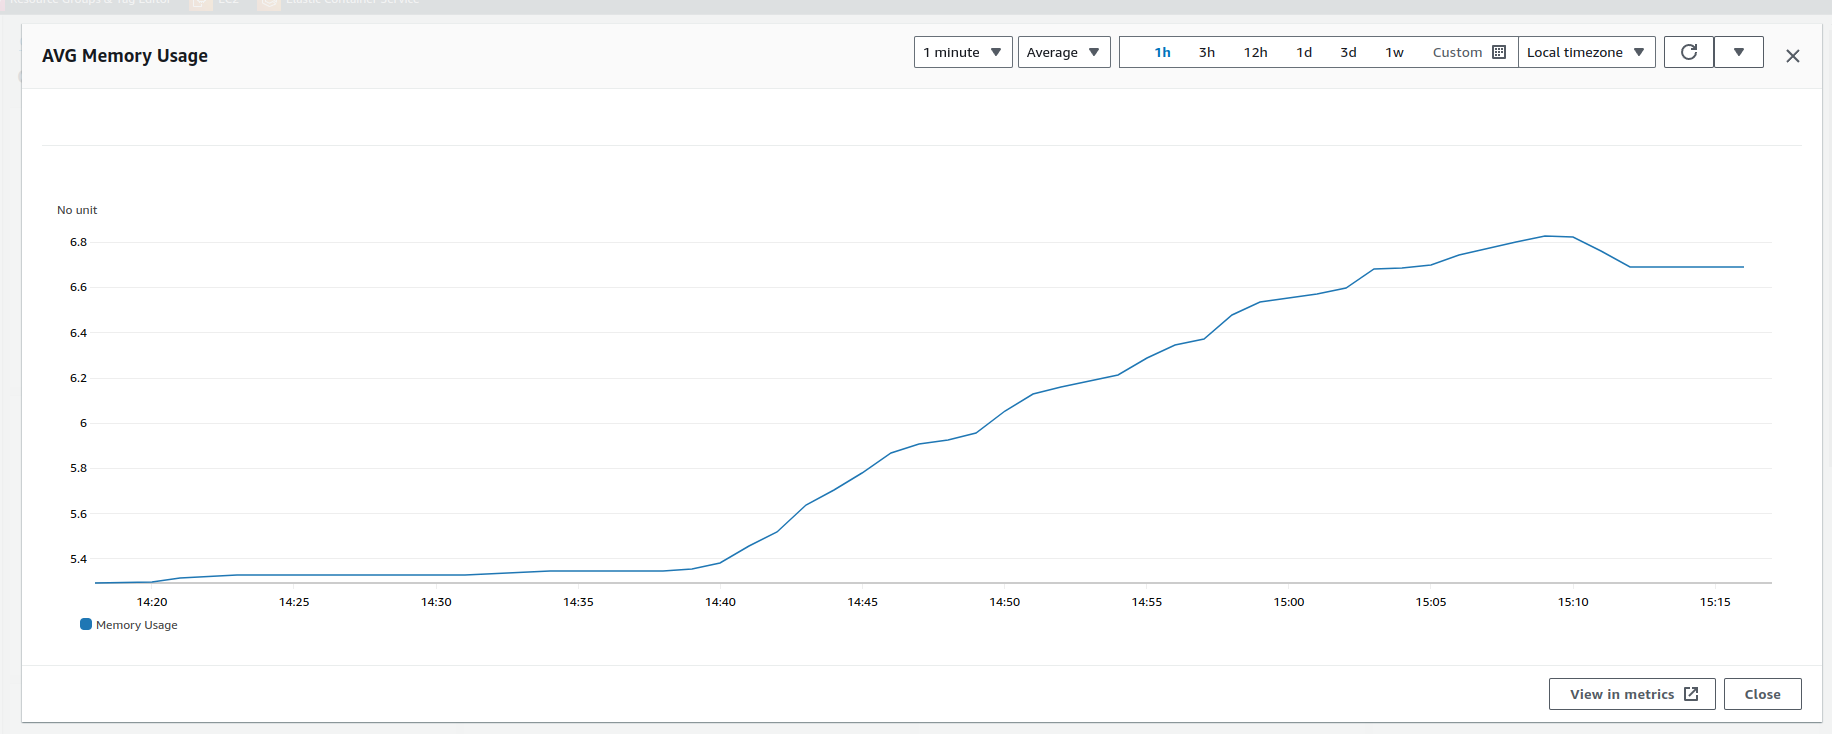
\includegraphics[width=0.8\textwidth]{media/memory-usage.png}
    \fonte{o autor}
    \label{fig:memory-utilization}
\end{figure}

\subsection{Tempo de Resposta}
Na \autoref{fig:response-time} é possível observar o tempo de resposta das requisições durante a simulação. Utilizando como base o P90, o tempo de resposta se manteve em torno de 1 segundo, um valor considerado aceitável. Esse valor também está abaixo do alvo de 2 segundos estabelecido anteriormente.

\begin{figure}[H]
    \centering
    \caption{Tempo de Resposta}
    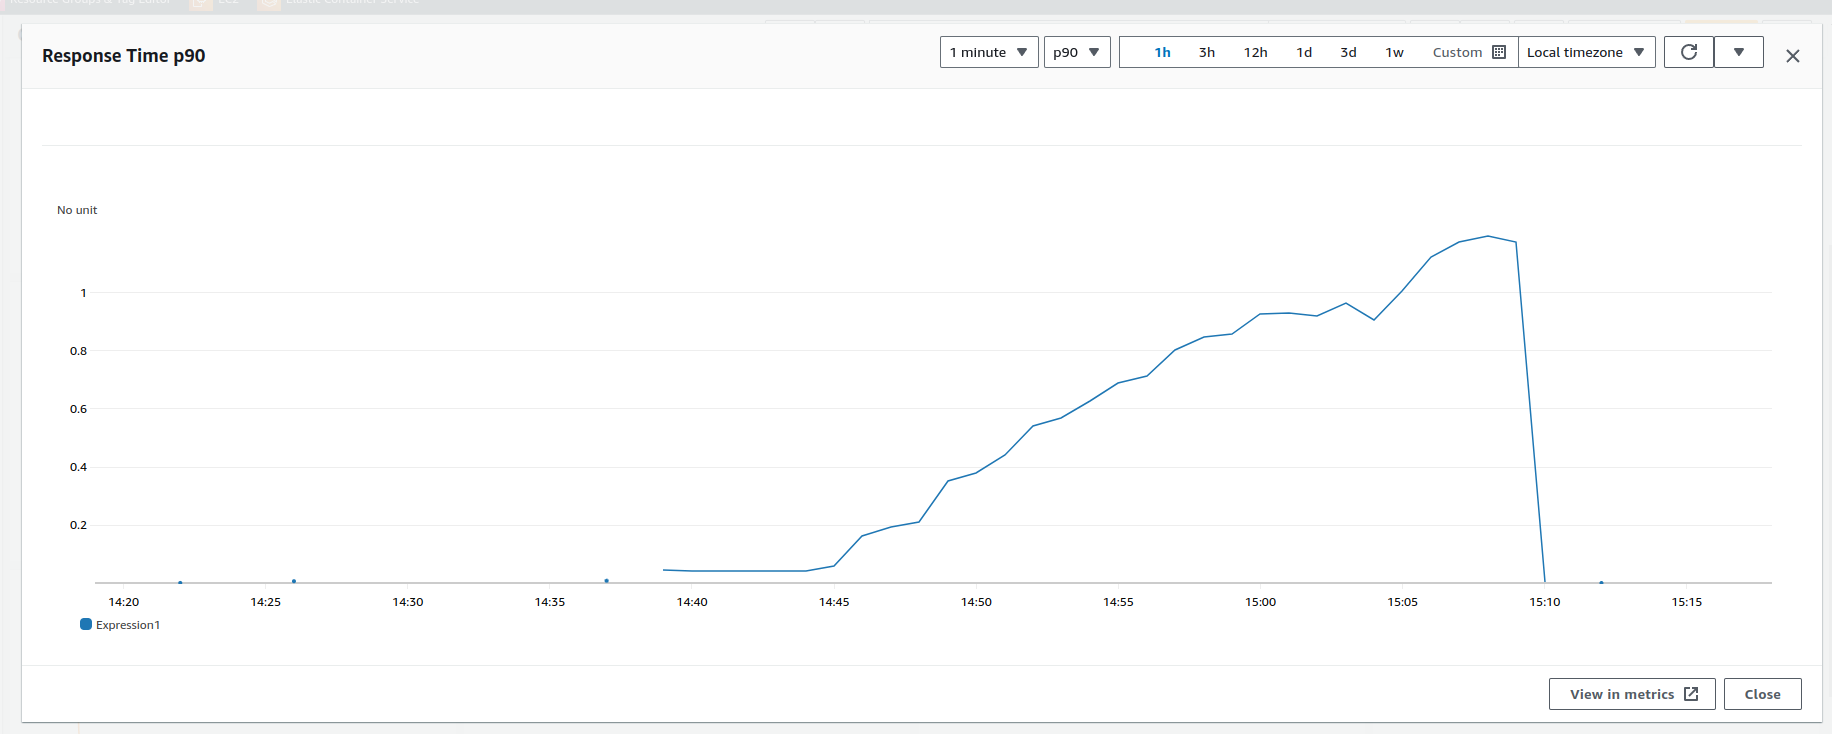
\includegraphics[width=0.8\textwidth]{media/response-time.png}
    \fonte{o autor}
    \label{fig:response-time}
\end{figure}

\subsection{Porcentagem de erros}
Na \autoref{fig:error-rate} é possível observar a porcentagem de erros durante a execução dos testes de carga. Durante toda a simulação, a porcentagem de erros se manteve em 0.2\% (média), indicando que o sistema é capaz de suportar um grande número de requisições sem impactar os usuários. Esse valor também está abaixo do alvo de 1\% estabelecido anteriormente.

\begin{figure}[H]
    \centering
    \caption{Porcentagem de Erros}
    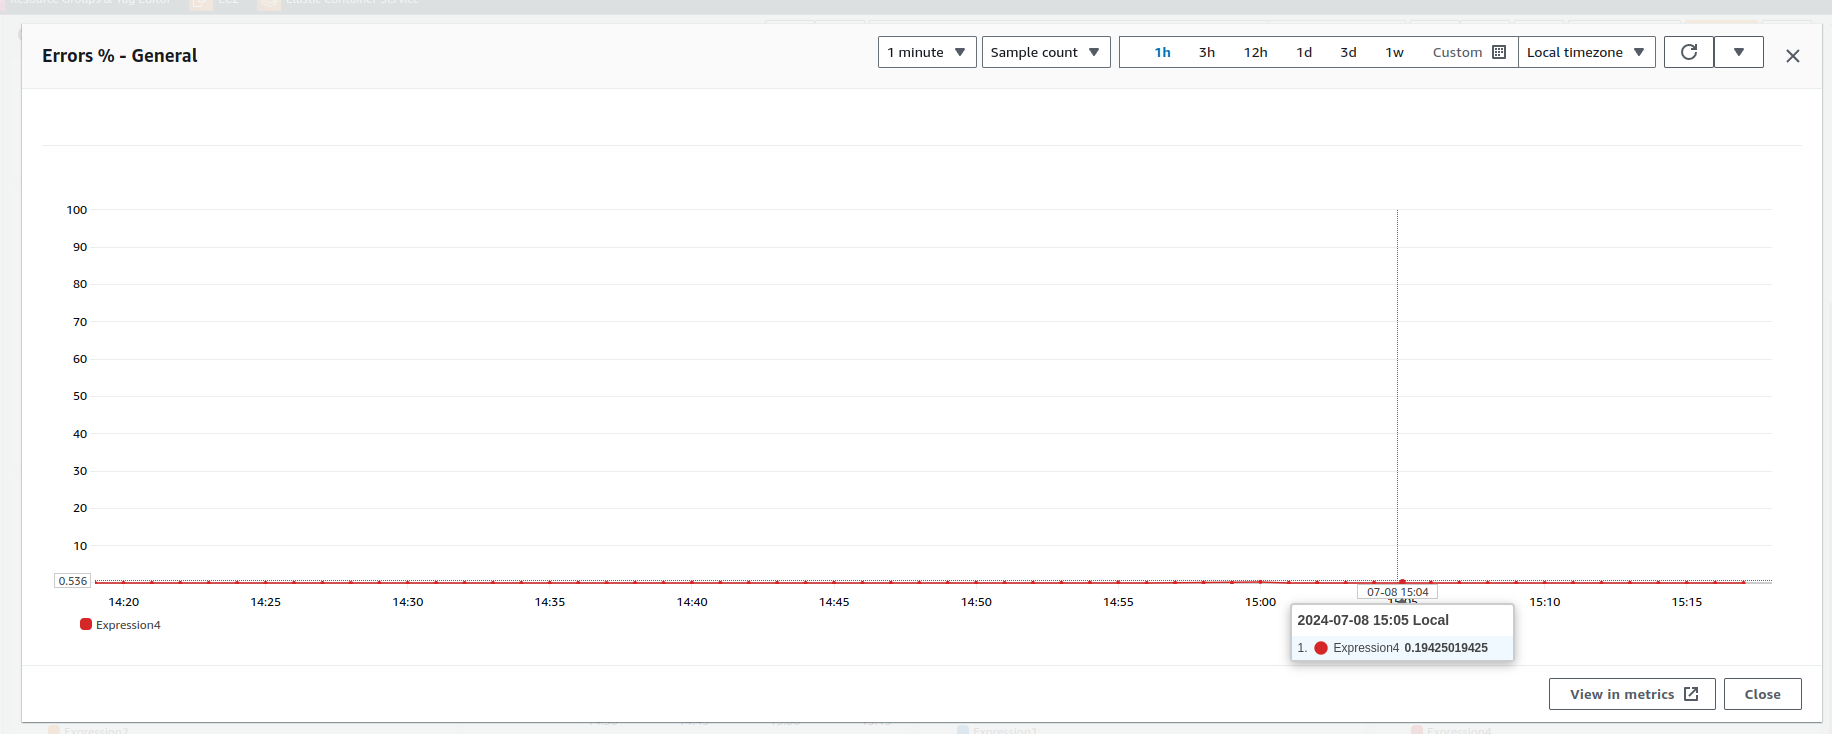
\includegraphics[width=0.8\textwidth]{media/errors.png}
    \fonte{o autor}
    \label{fig:error-rate}
\end{figure}

\section{Trabalhos Futuros}
Como trabalhos futuros, é possível destacar a construção de novos estudos de caso com a utilização de \acrshort{ddd} e \acrshort{ams} em outros contextos complexos como, por exemplo, sistemas financeiros, sistemas de logísticas e sistemas de saúde. Além disso, um trabalho futuro interessante seria a comparação de entre dois sistemas de domínios iguais, um desenvolvido com as técnicas apresentadas nesse trabalho e um outro somente com \acrshort{ddd} ou \acrshort{ams}. Assim, seria possível quantificar os benefícios e desvantagens da utilização dessas tecnologias em conjunto.

\section{Discussões}
Essa seção apresenta uma discussão geral sobre o processo de desenvolvimento do caso de uso com a utilização da \acrfull{ams} e \acrfull{ddd}. A utilização dessas tecnologias trouxe diversos desafios e benefícios ao desenvolvimento do sistema.

A separação de serviços em microsserviços permitiu que cada parte do sistema fosse desenvolvida de forma independente, facilitando a manutenção e evolução do sistema. Além disso, a utilização de \acrfull{ddd} permitiu que o domínio do negócio fosse modelado de forma mais clara e eficiente, facilitando o entendimento do sistema como um todo.

Da mesma forma, como cada microsserviço tem um foco específico, se torna mais fácil o entendimento de como cada parte do sistema funciona. Isso também facilita a escalabilidade do sistema, uma vez que é possível escalar apenas os serviços que estão sobrecarregados.

A utilização de \acrfull{ams} e \acrfull{ddd} trouxe diversos desafios ao desenvolvimento do sistema. O maior deles foi a necessidade de um maior esforço de \english{design upfront} para garantir a correta separação de serviços e a definição do domínio do negócio. Isso se deve ao fato de que a separação de serviços em microsserviços e a utilização de \acrfull{ddd} requerem um maior entendimento do negócio e da arquitetura do sistema.

Além disso, a complexidade aumentada para criação e execução de testes também foi um desafio. Como cada microsserviço é um sistema independente, é necessário criar testes para cada parte do sistema, o que aumenta a complexidade dos testes.

Outro desafio foi o maior custo computacional para executar o sistema localmente. Como cada microsserviço é uma aplicação independente, possui seu próprio processo em nível de sistema operacional, o que aumenta o custo computacional para executar o sistema localmente. Assim, os desenvolvedores precisam de máquinas mais potentes.

Por fim, a maior complexidade de deploy também foi um desafio. É necessário criar mais serviços, configurar máquinas virtuais, \english{load balancers} e banco de dados. Além disso, é importante configurar corretamente a rede para garantir a comunicação entre os serviços. Inicialmente, se tem um custo maior para manter o sistema em produção. Porém, com o crescimento do tráfego, a escalabilidade do sistema se torna mais fácil.

\chapter{Conclusão}
\label{cap:conclusão}

Este trabalho apresentou um estudo de caso sobre a utilização de \acrfull{ddd} e \acrfull{ams} no desenvolvimento de um sistema para uma locadora de veículos. O objetivo foi avaliar como essas tecnologias podem ser utilizadas para aumentar a escalabilidade e resiliência de sistemas complexos. Com base dos resultados obtidos com a execução dos testes de carga, é possível concluir que essa abordagem é eficaz para a construção de sistemas distribuídos. Além disso, nota-se como diferentes partes do sistema são expostos a tráfegos distintos, o que permite a escalabilidade independente de cada serviço.

Com a modelagem do sistema através de \acrshort{ddd}, foi possível definir limites claros entre os diferentes contextos do negócio com a utilização de \acrfull{bc}. Além disso, a utilização de \acrshort{ddd} permitiu a definição de um modelo de domínio rico e expressivo, que reflete de forma fiel as regras de negócio da locadora de veículos.

Por otro lado, o desenvolvimento deste estudo de caso trouxe diversos desafios como a necessidade de um maior esforço de \english{design upfront} para garantir a correta separação de serviços e a definição do domínio do negócio. Além disso, percebe-se uma maior complexidade para realização de testes e depuração de problemas, uma vez que o sistema é composto por diversos serviços independentes.

Este trabalho cumpriu com os objetivos propostos, na medida que apresentou uma estratégia para transformar requisitos funcionais em um \english{design} com \acrshort{ams} e \acrshort{ddd}, prover informações relevantes para definição dos estilo de comunicação adequado entre microsserviços e demonstrar desempenho e escalabilidade do sistema desenvolvido através de testes de carga.


\postextual

\bibliography{Referencias}

% Imprime uma página indicando o início dos apêndices
% \partapendices
\part*{Apêndices}

\begin{apendicesenv}


\chapter{Questionário de Avaliação do Protótipo}

\begin{figure}[H]
	\begin{Center}
		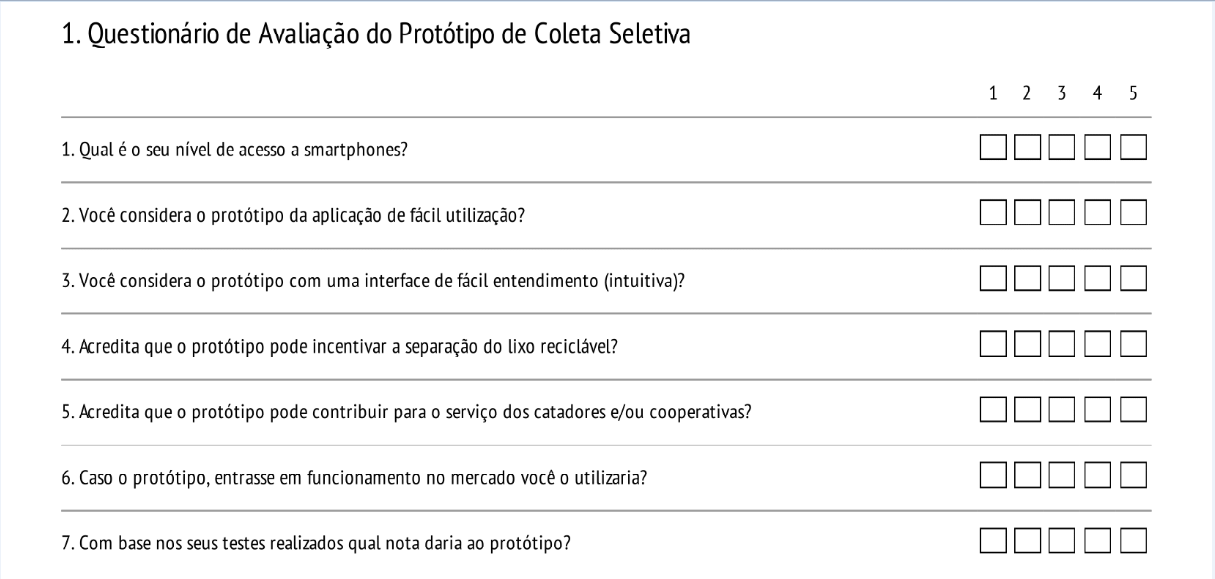
\includegraphics[width=6.00in]{media/questionariopaint.png}
		\label{fig:questionario}
	\end{Center}
\end{figure}

\chapter{Códigos fonte comentados}

\section{Salvar usuário catador no banco de dados}

O \autoref{cod:cadbanc} é responsável por salvar o usuário catador no \textit{firebase realtime database}. A linha 3 do \autoref{cod:cadbanc}, consiste na criação do nó (\textit{child}) denominado “Catadores”, onde cada catador possui um identificador (\textit{id}), onde seus dados são salvos (\textit{setValue}).

\begin{codigo}[H]
\begin{lstlisting}[language=Java]
public void salvar(){
    DatabaseReference databaseReference = ConfiguracaoFirebase.getFirebase();
    databaseReference.child("Catadores").child(getId()).setValue(this);
}
\end{lstlisting}
\caption{Salvar usuário catador no banco de dados}
\label{cod:cadbanc}
\end{codigo}


\section{Salvar usuário separador no banco de dados}

\begin{codigo}[H]
	\begin{lstlisting}[language=Java]
public void salvar(){
    DatabaseReference databaseReference = ConfiguracaoFirebase.getFirebase();
    databaseReference.child("Separadores").child(getId()).setValue(this);
}
   	\end{lstlisting}
   	\caption{Salvar usuário separador no banco de dados}
   	\label{cod:cadsep}
\end{codigo}

O \autoref{cod:cadsep} é responsável por salvar o usuário separador no \textit{firebase realtime database}. A linha 3 do \autoref{cod:cadbanc}, consiste na criação do nó (\textit{child}) denominado “Separadores”, onde cada separador possui um identificador (\textit{id}), onde seus dados são salvos (\textit{setValue}).


\section{Cadastrar usuário catador}

\begin{codigo}[H]
	\begin{lstlisting}[language=Java]
private void cadastrarCatador(){
    firebaseAuth = ConfiguracaoFirebase.getFirebaseAuth();
    firebaseAuth.createUserWithEmailAndPassword(
            catador.getEmail(),
            catador.getSenha()
    ).addOnCompleteListener(CadastroCatador.this, new OnCompleteListener<AuthResult>() {
        @Override
        public void onComplete(@NonNull Task<AuthResult> task) {
            if(task.isSuccessful()){
                Toast.makeText(CadastroCatador.this,"Sucesso ao cadastrar catador",Toast.LENGTH_LONG).show();
                FirebaseUser firebaseUser = task.getResult().getUser();
                catador.setId(firebaseUser.getUid());
                catador.salvar();
                startActivity(new Intent(CadastroCatador.this, Login.class));
       	\end{lstlisting}
       	\caption{Cadastrar usuário catador na aplicação}
       	\label{cod:cat}
\end{codigo}

O \autoref{cod:cat} consiste no cadastro do usuário catador. A função \textit{createUserWithEmailAndPassword}, que se encontra na linha 3, é responsável pela criação da autenticação dos usuário através do \textit{e-mail} e a senha. Em caso de sucesso, o sistema irá exibir a seguinte mensagem “Sucesso ao cadastrar catador” e o usuário será redirecionado para a tela de \textit{login}.

\section{Cadastrar usuário separador}

\begin{codigo}[H]
	\begin{lstlisting}[language=Java]
private void cadastrarSeparador(){
    firebaseAuth = ConfiguracaoFirebase.getFirebaseAuth();
    firebaseAuth.createUserWithEmailAndPassword(
            separador.getEmail(),
            separador.getSenha()
    ).addOnCompleteListener(CadastroSeparador.this, new OnCompleteListener<AuthResult>() {
        @Override
        public void onComplete(@NonNull Task<AuthResult> task) {
            if(task.isSuccessful()){
                Toast.makeText(CadastroSeparador.this,"Sucesso ao cadastrar separador",Toast.LENGTH_LONG).show();
                FirebaseUser firebaseUser = task.getResult().getUser();
                separador.setId(firebaseUser.getUid());
                separador.salvar();
                startActivity(new Intent(CadastroSeparador.this, Login.class));
       	\end{lstlisting}
       	\caption{Cadastrar usuário separador}
       	\label{cod:sep}
\end{codigo}

O \autoref{cod:sep} consiste no cadastro do usuário separador. A função \textit{createUserWithEmailAndPassword}, que se encontra na linha 3, é responsável pela criação da autenticação do usuário através do \textit{e-mail} e a senha. Em caso de sucesso, o sistema irá exibir a seguinte mensagem “Sucesso ao cadastrar separador” e o usuário será redirecionado para a tela de \textit{login}.

\section{Redefinir a senha}

\begin{codigo}[H]
	\begin{lstlisting}[language=Java]
	private void redefinirsenha(){
        firebaseAuth = FirebaseAuth.getInstance();
        firebaseAuth.sendPasswordResetEmail(recuperar.getEmail())
                .addOnCompleteListener(new OnCompleteListener<Void>() {
                    @Override
                    public void onComplete(@NonNull Task<Void> task) {
                        if(task.isSuccessful()) {
                            Toast.makeText(RecuperarSenha.this, "E-mail enviado.", Toast.LENGTH_LONG).show();
                            startActivity(new Intent(RecuperarSenha.this, Login.class));
                        }else{
                            Toast.makeText(RecuperarSenha.this,"E-mail nao cadastrado.",Toast.LENGTH_LONG).show();
                        }
                    }
                });
    }
    \caption{Redefinir a senha}
    \label{cod:senha}
 	\end{lstlisting}
\end{codigo}

O \autoref{cod:senha} consiste na redefinição da senha do usuário. A linha 3 verifica se o \textit{e-mail} informado pelo usuário está cadastrado no \textit{firebase auth}. Em caso de sucesso, o sistema irá enviar um \textit{e-mail} para a redefinição da senha e o usuário será redirecionado para a tela de \textit{login}. Caso contrário o sistema irá exibir a seguinte mensagem “\textit{E-mail} não cadastrado”.

\section{Deslogar usuário}
\begin{codigo}[H]
	\begin{lstlisting}[language=Java]
private void deslogarUsuario() {
        firebaseAuth.signOut();
        Toast.makeText(MapsActivity.this, "Usuario deslogado!", Toast.LENGTH_LONG).show();
        Intent intent = new Intent(MapsActivity.this, Login.class);
        startActivity(intent);
        finish();
    \end{lstlisting}
    \caption{Deslogar usuário}
    \label{cod:des}
\end{codigo}

O \autoref{cod:des} consiste no \textit{logout} do usuário. A função \textit{signOut} que encontra na linha 2 é responsável por desconectar o usuário da aplicação. A linha 3 tem a função de exibir para o usuário a seguinte mensagem "Usuario deslogado". A linha 4 tem o papel de redirecionar o usuário para a tela de \textit{login}.

\section{Validar separador}

\begin{codigo}[H]
	\begin{lstlisting}[language=Java]
private void validarSeparador() {
    firebaseAuth2 = ConfiguracaoFirebase.getFirebaseAuth();
    firebaseAuth2.signInWithEmailAndPassword(
        separador.getEmail(),
        separador.getSenha()
    ).addOnCompleteListener(new OnCompleteListener<AuthResult>() {
        @Override
        public void onComplete(@NonNull Task<AuthResult> task) {
            if (task.isSuccessful()) {
                FirebaseUser currentUser = FirebaseAuth.getInstance().getCurrentUser();
                assert currentUser != null;
                String id = currentUser.getUid();
                DatabaseReference j = FirebaseDatabase.getInstance().getReference().child("Separadores").child(id);
                j.addValueEventListener(new ValueEventListener() {
                    @Override
                    public void onDataChange(@NonNull DataSnapshot dataSnapshot)
                    {
                        String userType = (String) dataSnapshot.child("userType").getValue();
                        if (userType != null && userType.equals("Separadores")) {
                            Toast.makeText(Login.this, "Login efetuado com sucesso!", Toast.LENGTH_SHORT).show();
                            Intent intentResident = new Intent(Login.this, Materiais.class);
                            startActivity(intentResident);
                            finish();
                        }
                }
    	\end{lstlisting}
    	\caption{Validar separador}
    	\label{cod:valsep}
\end{codigo}

O \autoref{cod:valsep} consiste na validação do usuário separador. A verificação do tipo de usuário separador é realizada através da referência do nó "Separador", do identificador e do tipo de usuário.


\section{Validar catador}

\begin{codigo}[H]
	\begin{lstlisting}[language=Java]
private void validarCatador() {
    firebaseAuth2 = ConfiguracaoFirebase.getFirebaseAuth();
    firebaseAuth2.signInWithEmailAndPassword(
        catador.getEmail(),
        catador.getSenha()
    ).addOnCompleteListener(new OnCompleteListener<AuthResult>() {
        @Override
        public void onComplete(@NonNull Task<AuthResult> task) {
            if (task.isSuccessful()) {
                FirebaseUser currentUser = FirebaseAuth.getInstance().getCurrentUser();
                assert currentUser != null;
                String id = currentUser.getUid();
                DatabaseReference j = FirebaseDatabase.getInstance().getReference().child("Catadores").child(id);
                j.addValueEventListener(new ValueEventListener() {
                    @Override
                    public void onDataChange(@NonNull DataSnapshot dataSnapshot)
                    {
                        String userType = (String) dataSnapshot.child("userType").getValue();
                        if (userType != null && userType.equals("Catador")) {
                            Toast.makeText(Login.this, "Login efetuado com sucesso!", Toast.LENGTH_SHORT).show();
                            Intent intentResident = new Intent(Login.this, Servicos.class);
                            startActivity(intentResident);
                            finish();
                        }
                }
    	\end{lstlisting}
    	\caption{Validar catador}
    	\label{cod:valcat}
\end{codigo}

O \autoref{cod:valcat} consiste na validação do usuário catador. A verificação do tipo de usuário catador é realizada através da referência do nó "Catadores", do identificador e do tipo de usuário.

\section{Traçar rota}

\begin{codigo}[H]
	\begin{lstlisting}[language=Java]
	private void parseJSon(String data) throws JSONException {
        if (data == null)
            return;
        List<Route> routes = new ArrayList<Route>();
        JSONObject jsonData = new JSONObject(data);
        JSONArray jsonRoutes = jsonData.getJSONArray("routes");
        for (int i = 0; i < jsonRoutes.length(); i++) {
            JSONObject jsonRoute = jsonRoutes.getJSONObject(i);
            Route route = new Route();
            JSONObject overview_polylineJson = jsonRoute.getJSONObject("overview_polyline");
            JSONArray jsonLegs = jsonRoute.getJSONArray("legs");
            JSONObject jsonLeg = jsonLegs.getJSONObject(0);
            JSONObject jsonDistance = jsonLeg.getJSONObject("distance");
            JSONObject jsonDuration = jsonLeg.getJSONObject("duration");
            JSONObject jsonEndLocation = jsonLeg.getJSONObject("end_location");
            JSONObject jsonStartLocation = jsonLeg.getJSONObject("start_location");
            route.distance = new Distance(jsonDistance.getString("text"), jsonDistance.getInt("value"));
            route.duration = new Duration(jsonDuration.getString("text"), jsonDuration.getInt("value"));
            route.endAddress = jsonLeg.getString("end_address");
            route.startAddress = jsonLeg.getString("start_address");
            route.startLocation = new LatLng(jsonStartLocation.getDouble("lat"), jsonStartLocation.getDouble("lng"));
            route.endLocation = new LatLng(jsonEndLocation.getDouble("lat"), jsonEndLocation.getDouble("lng"));
            route.points = decodePolyLine(overview_polylineJson.getString("points"));
            routes.add(route);
        }
        listener.onDirectionFinderSuccess(routes);
    }
 	\end{lstlisting}
 	\caption{Traçar rota}
 	\label{cod:rot}
\end{codigo}

O \autoref{cod:rot} é responsável por traçar a rota informando sua distância e duração. 








\end{apendicesenv}

\begin{anexosenv}




\end{anexosenv}

\end{document}
